\documentclass[10pt,twoside,openany,hidelinks]{memoir}
\usepackage{memsty}
\usepackage{memlays}
\usepackage[paper=b5paper]{geometry}
\usepackage{graphicx}
\usepackage[utf8]{inputenc}
\usepackage[finnish]{babel}
\usepackage{multicol}
\usepackage[hypcap,font=small,format=hang,font=it,labelfont=bf]{caption}
\usepackage{marvosym}
\usepackage{textcomp} 
\usepackage{lipsum}
\usepackage{amssymb}
\usepackage{enumitem}
\usepackage[condensed]{cabin}
\usepackage{framed}
\usepackage{pdfpages}
\graphicspath{{graphics/}}

\addto\captionsfinnish{\def\figurename{}}
\makeatletter 
\renewcommand{\thefigure}{\arabic{chapter}.S\arabic{figure}}
\makeatother

\newcommand{\Rparagraph}[1]{\paragraph{#1}}

\DeclareUnicodeCharacter{21D2}{\(\Rightarrow\)}
\DeclareUnicodeCharacter{21E8}{\(\Rightarrow\)}
\DeclareUnicodeCharacter{2003}{ }
\DeclareUnicodeCharacter{20AC}{\EUR{}}
\DeclareUnicodeCharacter{00B0}{\textdegree}
\newcommand{\raisedrule}[2][0em]{\leaders\hbox{\rule[#1]{1pt}{#2}}\hfill}
\newcommand{\percent}{\%}

\setlist[itemize]{leftmargin=*}
\setlist[enumerate]{leftmargin=*}

\title{Laskuvarjohyppääjän opas}
\hypersetup{
    pdftitle = {Laskuvarjohyppääjän opas},
    pdfauthor = {SIL-opasryhmä}
}

\newenvironment{Figure}
  {\par\medskip\noindent\minipage{\linewidth}}
  {\endminipage\par\medskip}

\setstocksize{250mm}{176mm}
\setlength{\trimtop}{0mm} 
\setlength{\trimedge}{0mm}
\setbinding{7mm}
\setlrmarginsandblock{8mm}{*}{*}
\setulmarginsandblock{25mm}{20mm}{*}
\setmarginnotes{17pt}{51pt}{\onelineskip}
\setheadfoot{3\onelineskip}{2\onelineskip} 
\setheaderspaces{*}{\onelineskip}{*}
\checkandfixthelayout
\fixpdflayout

\settocdepth{section}
\setsecnumdepth{subsection}
\pagestyle{headings}
\makeevenhead{headings}{\textbf{\thepage}}{}{\leftmark}
\makeoddhead{headings}{\rightmark}{}{\textbf{\thepage}}
%% \makeheadrule{headings}{\textwidth}{\normalrulethickness}
\chapterstyle{wilsondob}
\setsecheadstyle{\LARGE\sffamily\raggedright}
\setsubsecheadstyle{\Large\sffamily\raggedright}
\setsubsubsecheadstyle{\large\sffamily\raggedright}
\setlength{\parindent}{0pt}
\setlength{\parskip}{0.5\onelineskip}
\setlength{\columnsep}{6mm}
\renewcommand*{\chapnumfont}{\sffamily\Huge}%
\renewcommand*{\printchapternum}{\raggedleft\chapnumfont \thechapter\quad}%
\renewcommand*{\afterchapternum}{}%
\renewcommand*{\chaptitlefont}{\chapnumfont}%
\renewcommand*{\printchapternonum}{\raggedleft}
\renewcommand*{\partnamefont}{\sffamily\fontsize{36pt}{1em}\bfseries}
\renewcommand*{\partnumfont}{\sffamily\fontsize{36pt}{1em}\bfseries}
\renewcommand*{\parttitlefont}{\sffamily\fontsize{42pt}{1em}\bfseries}

\urlstyle{rm}

%% title page
\newcommand*{\titleDB}{\begingroup% Design of Books, by Adrian Wilson
%\LXfont{ppl}%   Palatino/Palladio
\tdrop = 0.14\txtheight
%\centering
%\vspace*{\tdrop}
\sffamily
\raggedleft
\Large
{20.4.2014} 
\Huge
\vspace*{\baselineskip} \\
{Suomen Ilmailuliitto}\\[0.3\baselineskip]
{Laskuvarjotoimikunta}\\[0.3\baselineskip]
{Koulutus- ja turvallisuuskomitea}\\[0.2\baselineskip]
\hrulefill 
\vspace*{0.4\baselineskip} \\
\raggedright
\parttitlefont
{LASKUVARJOHYPPÄÄJÄN}\\[\baselineskip]
{OPAS}\\[2\baselineskip]
%\begin{vplace}
\LARGE
{Toimittanut}\\[0.3\baselineskip]
{Opastyöryhmä 2013-2014}\\[0.3\baselineskip]
\vfill
\LARGE
{Lähetä palautetta:}\\
{www.laskuvarjotoimikunta.fi/opaspalaute}\\
%\end{vplace}
\endgroup}

\begin{document}
\frontmatter

\pagestyle{empty}
\titleDB
\newpage

\pagestyle{headings}
\tableofcontents

\chapter{Tervetuloa Taivaalle}
\label{tervetuloa-taivaalle}
\thispagestyle{headings}
\begin{multicols}{2}
\input{tervetuloa-taivaalle.tex}\end{multicols}

\chapter{Laskuvarjohyppykoulutus}
\label{laskuvarjohyppykoulutus}
\thispagestyle{headings}
\begin{multicols}{2}
\input{laskuvarjohyppykoulutus.tex}\end{multicols}

\mainmatter\midsloppy\part{Alkeiskoulutus}\chapter{Yhteenveto: Alkeiskoulutus}
\label{yhteenveto-alkeiskoulutus}
\thispagestyle{headings}
\begin{multicols}{2}

Alkeisoppilaan kelpoisuus on voimassa vuoden myöntämispäivämäärästä. Jos kelpoisuus vanhenee, oppilaan tulee uusia teoriakoe ja käytännön näytteet ennen hyppäämistä. Oppilaan on saavutettava jokaisella hyppysuorituksella välttämättömät oppimistavoitteet hyväksytysti, jotta suoritus voidaan hyväksyä. 

\section{ Hyppysuoritukset, NOVA }
\label{yhteenveto-alkeiskoulutus-hyppysuoritukset-nova}

\begin{itemize}
\item  Taso 1 (\ref{nova-alkeiskoulutuksen-suoritukset-taso-1-tottuminen-vapaapudotukseen} s.\pageref{nova-alkeiskoulutuksen-suoritukset-taso-1-tottuminen-vapaapudotukseen}) 
\item  Taso 2 (\ref{nova-alkeiskoulutuksen-suoritukset-taso-2-asennon-hallinta} s.\pageref{nova-alkeiskoulutuksen-suoritukset-taso-2-asennon-hallinta}) 
\item  Taso 3 (\ref{nova-alkeiskoulutuksen-suoritukset-taso-3-stabiili-vapaapudotus} s.\pageref{nova-alkeiskoulutuksen-suoritukset-taso-3-stabiili-vapaapudotus}) 
\item  Taso 4 (\ref{nova-alkeiskoulutuksen-suoritukset-taso-4-kaannokset-90deg} s.\pageref{nova-alkeiskoulutuksen-suoritukset-taso-4-kaannokset-90deg}) 
\item  Taso 5 (\ref{nova-alkeiskoulutuksen-suoritukset-taso-5-kaannokset-360deg} s.\pageref{nova-alkeiskoulutuksen-suoritukset-taso-5-kaannokset-360deg}) 
\item  Taso 6 (\ref{nova-alkeiskoulutuksen-suoritukset-taso-6-irtiuloshyppy} s.\pageref{nova-alkeiskoulutuksen-suoritukset-taso-6-irtiuloshyppy}) 
\item  Taso 7 (\ref{nova-alkeiskoulutuksen-suoritukset-taso-7-puolisarja} s.\pageref{nova-alkeiskoulutuksen-suoritukset-taso-7-puolisarja}) 
\item  15'' lyhyt vapaa (\ref{nova-alkeiskoulutuksen-suoritukset-15-lyhyt-vapaa} s.\pageref{nova-alkeiskoulutuksen-suoritukset-15-lyhyt-vapaa}) 
\end{itemize}
\section{ Hyppysuoritukset, PL }
\label{yhteenveto-alkeiskoulutus-hyppysuoritukset-pl}

\begin{itemize}
\item  3 pakkolaukaisua (\ref{pl-alkeiskoulutuksen-suoritukset-pakkolaukaisu} s.\pageref{pl-alkeiskoulutuksen-suoritukset-pakkolaukaisu}) 
\item  3 harjoitusvetoa (\ref{pl-alkeiskoulutuksen-suoritukset-harjoitusveto} s.\pageref{pl-alkeiskoulutuksen-suoritukset-harjoitusveto}) 
\item  3'' itseaukaisu (\ref{pl-alkeiskoulutuksen-suoritukset-itseaukaisu-3} s.\pageref{pl-alkeiskoulutuksen-suoritukset-itseaukaisu-3}) 
\item  5'' itseaukaisu (\ref{pl-alkeiskoulutuksen-suoritukset-itseaukaisu-5} s.\pageref{pl-alkeiskoulutuksen-suoritukset-itseaukaisu-5}) 
\item  10'' itseaukaisu (\ref{pl-alkeiskoulutuksen-suoritukset-10} s.\pageref{pl-alkeiskoulutuksen-suoritukset-10}) 
\end{itemize}
\section{ Muut suoritukset }
\label{yhteenveto-alkeiskoulutus-muut-suoritukset}

\begin{itemize}
\item  Peruskoulutuksen teoriakoe. Opiskeltava alue on luvusta \textit{Yhteenveto: Peruskoulutus} (\ref{yhteenveto-peruskoulutus} s.\pageref{yhteenveto-peruskoulutus}) lukuun \textit{Peruskoulutuksen muut suoritukset} (\ref{peruskoulutuksen-muut-suoritukset} s.\pageref{peruskoulutuksen-muut-suoritukset}). 
\end{itemize}
\section{ NOVA-suoritusten aikarajat }
\label{yhteenveto-alkeiskoulutus-nova-suoritusten-aikarajat}

\begin{itemize}
\item  Jos tasokoulutuksen aikana oppilaalle tulee 30 vrk tai sitä pitempi hyppytauko, hänen on uusittava edellinen taso, kuitenkin enintään 3. taso.  
\item  NOVA-oppilaan on hypättävä alkeiskoulutuksen viimeinen hyppy (15'') \textbf{neljäntoista} vuorokauden sisällä viimeisestä tasohypystä, muuten hän joutuu uusimaan tason 7. 
\end{itemize}
\section{ PL-suoritusten aikarajat }
\label{yhteenveto-alkeiskoulutus-pl-suoritusten-aikarajat}

\begin{itemize}
\item  Jos alkeiskoulutuksen aikana oppilaalle tulee 30 vrk tai sitä pidempi hyppytauko, hänen on hypättävä totuttelusuoritus ennen seuraavaa hyppyä riippuen edellisestä suorituksesta: 
	\begin{itemize}
	\item  PL tai HV ⇨ PL 
	\item  3'', 5'' tai 10'' ⇨ HV 
	\end{itemize}
\item  Ensimmäinen itseaukaisuhyppy on hypättävä viimeistään seuraavan vuorokauden aikana viimeisestä hyväksytystä harjoitusvetosuorituksesta. 
\end{itemize}
\end{multicols}

\chapter{Laskuvarjokalusto ja hyppyvarusteet}
\label{laskuvarjokalusto-ja-hyppyvarusteet}
\thispagestyle{headings}
\begin{multicols}{2}
\section{ Laskuvarjokokonaisuus }
\label{laskuvarjokalusto-ja-hyppyvarusteet-laskuvarjokokonaisuus}


\begin{figure*}[]\centering\includegraphics[width=0.7\textwidth]{Paavarjon-osat.jpg}\caption{Päävarjon osat: 1. Kupu 2. Tunnelipari 3. Kuvun takahelma 4. Stabilisaattori 5. Kantopunokset 6. Ohjauspunokset 7. Slider 8. Kantohihnat 9. Apuvarjo}\end{figure*} 


Laskuvarjokokonaisuuteen kuuluu reppu-valjasyhdistelmä sekä kaksi varjoa: pää- ja varavarjo. Molemmat näistä ovat liitovarjoja, jotka ovat muodoltaan siiven kaltaisia. Niiden liitosuhde on noin 3:1, eli liitäessään kolme metriä eteenpäin varjo vajoaa metrin.  


\begin{Figure}\centering\includegraphics[width=0.7\textwidth]{Reppu-valjas-etu.png}\captionof{figure}{Wings-reppuvaljasyhdistelmä hyppääjän päällä}\end{Figure} 

\subsection{ Päävarjo }
\label{laskuvarjokalusto-ja-hyppyvarusteet-paavarjo}


Päävarjo, joka koostuu kuvusta, punoksista ja sliderista, on kantohihnojen välityksellä kiinni valjaissa kolmirengaslukkojen avulla. Kupu on rakennettu tunneleista, joiden toinen pää on umpinainen. Eripituisilla kantopunoksilla kuvun kohtauskulma pidetään sellaisena, että etureuna on takareunaa hieman alempana. Liitovarjo muodostaa nostovoimaa samalla tavalla kuin lentokoneen siipi. 

\subsection{ Varavarjo }
\label{laskuvarjokalusto-ja-hyppyvarusteet-varavarjo}


Varavarjo on rakenteeltaan ja toiminnaltaan samanlainen kuin päävarjo. Varavarjoa käytettäessä laskeutumispaikka saattaa olla muualla kuin laskeutumisalueella. Tämän vuoksi alastuloasennon on oltava hyvä ja tarvittaessa on tehtävä maahantulokierähdys. 

\section{ Reppu-valjasyhdistelmä }
\label{laskuvarjokalusto-ja-hyppyvarusteet-reppu-valjasyhdistelma}


\begin{Figure}\centering\includegraphics[width=0.6\textwidth]{Reppuvaljasyhdistelma.png}\captionof{figure}{1. Valjaan pystyhihnojen säätösoljet 2. Päävarjon irtipäästöpampula 3. Varavarjon avauskahva 4. Rintahihna 5. Varavarjon pakkolaukaisuhihna RSL 6. Koukkupuukko (sijainti voi vaihdella) 7. Kolmirengasolkalukot 8. FXC-automaattilaukaisimen säätöyksikkö (mikäli käytössä joku muu, merkitse säätöyksikön paikka kuvaan) 9. Reisihihnat}\end{Figure} 


\begin{Figure}\centering\includegraphics[width=0.6\textwidth]{Reppu-nova.pdf}\captionof{figure}{10. Päävarjon apuvarjo 11. Päävarjon reppu 12. Varavarjon reppu 13. Päävarjon läppä 14. Päävarjon avauskahva hyppymestarille (NOVA-kahva)}\end{Figure} 


\begin{Figure}\centering\includegraphics[width=0.6\textwidth]{Reppu-pl.pdf}\captionof{figure}{10. PL-hihna 11. Päävarjon reppu 12. Varavarjon reppu 13. Päävarjon läppä}\end{Figure} 

\section{ Lisälaitteet }
\label{laskuvarjokalusto-ja-hyppyvarusteet-lisalaitteet}


Pää- ja varavarjon lisäksi valjaissa on laitteita lisäämässä hyppääjän turvallisuutta. Näiden laitteiden tarkoituksena on varmistaa varavarjon aukeaminen. 


Varavarjon pakkolaukaisuhihnan (Reserve Static Line, RSL) tarkoituksena on varmistaa varavarjon avautuminen päävarjon irrottua valjaista. Järjestelmä liittää päävarjon kantohihnan ja varavarjon aukaisujärjestelmän yhteen. Hyppääjän on mahdollista vapauttaa varavarjon pakkolaukaisuhihna avaamalla päävarjon kantohihnaan kytketty pikalukko. 


Kun päävarjon kantohihnat ovat päävarjon irtipäästön (\ref{paavarjon-vajaatoiminnot-varavarjon-kaytto} s.\pageref{paavarjon-vajaatoiminnot-varavarjon-kaytto}) jälkeen irronneet kolmirengaslukoista, päävarjo vetää irrotessaan varavarjon pakkolaukaisuhihnasta ja avaa varavarjon. Varavarjon pakkolaukaisuhihna on kuitenkin vain apuväline. Hyppääjän on aina avattava varavarjo vetämällä varavarjon kahvasta! 


\begin{Figure}\centering\includegraphics[width=0.7\textwidth]{Kolmirengaslukko.jpg}\captionof{figure}{Kolmirengaslukko}\end{Figure} \begin{Figure}\centering\includegraphics[width=0.7\textwidth]{Kolmirengaslukko-auki.jpeg}\captionof{figure}{Kolmirengaslukko on auennut. Päävarjon kantohihna vetää irrotessaan RSL-hihnasta.}\end{Figure} 


Toinen lisälaite varavarjon aukaisuun on automaattilaukaisin (Automatic Activation Device, AAD). Käytössä on kahta eri tyyppiä: mekaaninen (FXC) ja elektroninen (Cypres ja Vigil). Laitteiden tarkoitus on avata varavarjo, jos hyppääjä putoaa liian kovalla vauhdilla liian matalalla. Molemmat laitteet on säädetty toimimaan määrätyssä korkeudessa (n. 300 m).  


Oppilaan ollessa kyseessä vain hyppymestarilla on oikeus säätää automaattilaukaisinta. FXC:n säätölaitteessa on JUMP/OFF-nuppi, jonka on koko ajan oltava JUMP-asennossa. On olemassa kaksi tilannetta, joissa FXC:n JUMP/OFF-nuppi käännetään OFF-asentoon: 

\begin{itemize}
\item  Koneella alas tultaessa hyppymestarin käskystä 
\item  Laskeuduttaessa veteen (\ref{mahdolliset-vaaratilanteet-laskeutuminen-veteen} s.\pageref{mahdolliset-vaaratilanteet-laskeutuminen-veteen}) 
\end{itemize}

\begin{Figure}\centering\includegraphics[width=0.7\textwidth]{AAD-Cypres.jpg}\captionof{figure}{Cypres-automaattilaukaisimen käyttöyksikkö}\end{Figure} 

\section{ Muut hyppytoiminnassa käytettävät varusteet }
\label{laskuvarjokalusto-ja-hyppyvarusteet-muut-hyppytoiminnassa-kaytettavat-varusteet}

\begin{itemize}
\item  Kova kypärä, jossa kiinnityshihna on kypärän ulkopuolella. 
\item  Radiovastaanotin on oltava ainakin kolmella ensimmäisellä hypyllä. 
\item  Suojalasit suojaavat silmiä viimalta ja roskilta. 
\item  Haalari, jossa ei saa olla tarttuvia taskuja tai ulokkeita, jotka voivat takertua johonkin tai joista hyppääjä voi vahingossa ottaa kiinni kahvoista kiinni ottaessaan. Haalarin alle puetaan säähän sopiva vaatetus, joka ei haittaa liikkumista. 
\item  Sormikkaat ovat pakolliset oppilailla. Niiden on oltava lämpimät, mutta ei liian paksut eikä liukkaat. 
\item  Kengät, joiden on oltava hyppytoimintaan soveltuvat (ei koukkuja tms.). 
\item  Korkeusmittari, joka nollataan maassa. Mittari kiinnitetään rintahihnaan tai käteen. 
\item  Koukkupuukkoa käytetään takertumien selvittämiseen sotkeutumis- tai törmäämistilanteissa. 
\item  Pelastusliivi puetaan koulutuspäällikön harkinnan mukaan, jos hyppypaikalla on ilmeinen hukkumisvaara. 
\end{itemize}

Hypyn aikana mukana ei saa olla mitään tarpeetonta (esimerkiksi avaimet, kynä tai matkapuhelin). Lisäksi aina hyppäämään tultaessa on oltava mukana hyppypäiväkirja. 

\section{ Hyppyvarusteiden käsittely }
\label{laskuvarjokalusto-ja-hyppyvarusteet-hyppyvarusteiden-kasittely}


Suojaa varjoa auringonvalolta, kosteudelta ja likaantumiselta. Nosta valjaita olkahihnoista ja varo tarttumasta aukaisukahvoihin sekä vaijereiden suojaputkiin. Varjoa ei tule heitellä, laahata eikä sen päällä tule istua. Älä tupakoi, kun olet pukenut valjaat päälle. 


Oppilaan päävarjon pakkaamista saa valvoa henkilö, jolla on itsenäisen hyppääjän kelpoisuus. Oppilaan käytössä olevan päävarjon pakkauksista ja pakkaustarkistuksista pidetään kirjaa. Varavarjon saa pakata vain siihen koulutuksen saanut henkilö. Varusteet palautetaan aina hypyn jälkeen omille paikoilleen. 

\section{ 3X3 -tarkastus }
\label{laskuvarjokalusto-ja-hyppyvarusteet-3x3-tarkastus}


Peruskoulutusvaiheessa oppilaalle opetetaan varusteiden perusteellinen tarkastus, mutta itseaukaisuvaiheessa varjon perustarkastus voidaan tiivistää 3X3 -tarkastukseen (kolme kolmea -tarkastus): 

\begin{enumerate}[label=\bfseries \arabic*)]
\item  Tarkastetaan, että solkia on kiinni kolme: 
	\begin{itemize}
	\item  Vasemman jalkahihnan solki 
	\item  Oikean jalkahihnan solki 
	\item  Rintahihnan solki 
	\end{itemize}
\item  Tarkastetaan, että kahvoja on kolme ja ne ovat kiinni: 
	\begin{itemize}
	\item  Päävarjon avauskahva 
	\item  Päävarjon irtipäästöpampula 
	\item  Varavarjon avauskahva 
	\end{itemize}
\item  Tarkastetaan, että kolmirengaslukot ovat kiinni ja oikein. 
\end{enumerate}
\end{multicols}

\chapter{Hyppytapahtuma}
\label{hyppytapahtuma}
\thispagestyle{headings}
\begin{multicols}{2}
\section{ Valmistautuminen hyppyyn }
\label{hyppytapahtuma-valmistautuminen-hyppyyn}


Hyppytapahtuma ei suinkaan ala siitä, kun poistutaan koneesta ilmassa. Jotta kaikki sujuisi hyvin, on tärkeää huolehtia myös valmisteluista. Päätös hypätä on hyvä tehdä jo edellisenä päivänä, sillä näin ehtii henkisesti valmistautua tulevaan suoritukseen. Riittävä yöuni ja ravinto ovat myös tärkeitä – väsyneenä tai nälkäisenä keskittyminen on vaikeaa. 


Ennen hyppäämään kirjoittautumista (pokalistan täyttöä) kootaan kaikki tarvittavat varusteet ja ilmoittaudutaan hyppäämään. Varusteita on hyvä sovittaa päälle, jotta niihin voi tehdä tarvittavat säädöt ajoissa ennen koneelle lähtöä. Suoritusta harjoitellaan joko itsenäisesti tai hyppymestarin kanssa. 


Mikäli mahdollista, seuraa ennen omaa pokaasi toisten hyppääjien ohjailua varjon varassa nähdäksesi ylä- ja pintatuulien vaikutuksen ohjaamiseen ja laskeutumiseen. 


Ennen koneelle menoa hyppymestari tarkastaa, että varusteet on puettu oikein päälle. Tarkastuksen jälkeen varusteita \textbf{ei saa säätää} ilman hyppymestarin lupaa! Vallitsevan tuulen mukainen ohjauskuvio (\ref{hyppytapahtuma-laskeutumiskuvio} s.\pageref{hyppytapahtuma-laskeutumiskuvio}) käydään vielä läpi ennen koneelle menoa. Oppilaat saavat mennä koneelle vain hyppymestarin johdolla. 

\subsection{ Toiminta koneessa }
\label{hyppytapahtuma-toiminta-koneessa}


Kone kuormataan yleensä käänteisessä järjestyksessä eli se, joka menee koneeseen ensimmäisenä, hyppää viimeisenä (poikkeuksena hyppymestari). Varo varusteiden tarttumista koneessa oleviin ulokkeisiin aina koneessa liikkuessasi. Suojaa erityisesti varjojen aukaisukahvoja myös muiden liikkuessa. Jos takerrut kiinni johonkin, älä revi itseäsi irti väkisin, vaan ilmoita asiasta hyppymestarille. Vältä turhaa liikkumista. Pidä mahdolliset istuinvyöt kiinni, kunnes hyppymestari aukaisee ne tai antaa luvan aukaisuun. Ilmailumääräyksen OPS M6-1 perusteella ilma-aluksella saa kuljettaa sen päällikön ja hyppääjien suostumuksella ja omalla vastuulla enintään kymmentä hyppääjää ilman istuinvyötä.  


Jos lennon aikana huomaat omissa tai muiden varusteissa jotain poikkeavaa, ilmoita siitä heti hyppymestarille. Keskity omaan hyppyysi. Huomioi muut koneessa olijat äläkä häiritse heidän keskittymistään. Koneen päällikkö on lentäjä, mutta sinun päällikkösi on hyppymestari. Lähestyttäessä uloshyppypaikkaa kone lentää tuuliolosuhteiden perusteella määriteltyä linjaa. Hyvissä ajoin ennen uloshyppypaikkaa hyppymestari tarkastaa vielä oppilaiden varusteet. 

\section{ Uloshyppy Cessna 206, pakkolaukaisu }
\label{hyppytapahtuma-uloshyppy-cessna-206-pakkolaukaisu}


Hyppymestarin komennolla OVELLE! siirrytään (varoen repun osumista koneeseen) ovelle uloshyppyasentoon. Komennolla MENE! ponnistetaan irti koneesta, otetaan hyvä taivutus ja delta-asento sekä aletaan laskea. Rintamasuunnan on pysyttävä koko ajan suoraan koneen lentosuuntaan. 


\begin{Figure}\centering\includegraphics[width=0.7\textwidth]{206UH1.jpeg}\captionof{figure}{Hyppääjä on siirtymässä ovelle uloshyppyasentoon}\end{Figure} 


Uloshypyssä maa vetää helposti katsetta puoleensa. Jos katsoo maahan eikä koneeseen, taivutus todennäköisesti kääntyy väärin päin. Ihmisen vartalo kääntyy yleensä katseen suuntaan, joten kun uloshypyn aikana katsoo ylös koneeseen, niin vartalo on taipunut oikeanlaiselle kaarelle. Taivutus lähtee lantiosta (myös selkä ja niska). 


Tärkeintä uloshypyssä on taivutus. Delta-asennossa kädet ovat n. 45 astetta irti kyljistä, olkapäät takana. Jalat pidetään noin hartioiden levyisessä haara-asennossa ja vain hiukan koukistettuna. 


Laskeminen on tärkeää opetella heti alusta alkaen, sillä se on käytännössä ainoa tapa säilyttää ajantaju tässä vaiheessa hyppyuraa. Laskeminen tapahtuu ääneen huutamalla (101...105). Uloshyppyharjoituksissa opetellaan oikeaa rytmiä, joten ei huudeta vain numeroita vaan sekunteja. Ilmassa muutama sekunti voi tuntua hyvinkin pitkältä ajalta. 


\begin{Figure}\centering\includegraphics[width=0.7\textwidth]{206UH2.jpeg}\captionof{figure}{Hyppääjä on ponnistanut irti koneesta.}\end{Figure} 


Onnistuneen uloshypyn päätekijät ovat: 

\begin{itemize}
\item  Asettautuminen hyvään uloshyppyasentoon ovelle (katse ylös koneeseen) 
\item  Riittävä ponnistus ja rintamasuunta lentosuuntaan  
\item  Hyvä ja symmetrinen delta-asento sekä voimakas taivutus ja katse ylös koneeseen 
\end{itemize}
\section{ Uloshyppy Streevakone, pakkolaukaisu }
\label{hyppytapahtuma-uloshyppy-streevakone-pakkolaukaisu}


Hyppymestarin komennolla OVELLE! siirrytään ovelle. Komennolla MENE! siirrytään (varoen repun osumista koneeseen) roikkumaan streevalle uloshyppyasentoon, irrottaudutaan koneesta ja pidetään hyvä taivutus sekä X-asento ja aletaan laskea. Rintamasuunnan on pysyttävä koko ajan suoraan koneen lentosuuntaan. 


\begin{Figure}\centering\includegraphics[width=0.7\textwidth]{Streeva-UH1.jpeg}\captionof{figure}{Hyppääjä on siirtynyt streevalle uloshyppyasentoon}\end{Figure} 


Uloshypyssä maa vetää helposti katsetta puoleensa. Jos katsoo maahan eikä koneeseen, taivutus kääntyy todennäköisesti väärin päin. Ihmisen vartalo kääntyy yleensä katseen suuntaan, joten kun katsoo uloshypyn aikana ylös kohti konetta, vartalo on taipunut oikeanlaiselle kaarelle. Taivutus lähtee lantiosta (myös selkä ja niska). 


Mikäli taivutuksesi syystä tai toisesta häviää, voit korjata tilanteen helposti: taivuttamalla. 


Tärkeintä uloshyppyasennossa ja uloshypyssä on siis taivutus. X-asennossa kädet ovat ylhäällä levitettyinä, olkapäät takana. Jalat pidetään noin hartioiden levyisessä haara-asennossa ja vain hiukan koukistettuna. 


Laskeminen on tärkeää opetella heti alusta alkaen, sillä se on käytännössä ainoa tapa säilyttää ajantaju tässä vaiheessa hyppyuraa. Laskeminen tapahtuu ääneen huutamalla (101...105). Uloshyppyharjoituksissa opetellaan oikeaa rytmiä, joten ei huudeta vain numeroita vaan sekunteja. Ilmassa muutama sekunti voi tuntua hyvinkin pitkältä ajalta. 


\begin{Figure}\centering\includegraphics[width=0.7\textwidth]{StreevaUH2.jpeg}\captionof{figure}{Hyppääjä on irroittautunut koneesta.}\end{Figure} 


Onnistuneen uloshypyn päätekijät ovat: 

\begin{itemize}
\item  Asettautuminen hyvään ja symmetriseen uloshyppyasentoon (X-asento, taivutus ja katse ylös koneeseen) 
\item  Käsien yhtäaikainen irrottaminen ja rintamasuunta lentosuuntaan  
\item  Hyvä ja symmetrinen X-asento sekä voimakas taivutus ja katse ylös koneeseen 
\end{itemize}
\section{ Uloshyppy NOVA }
\label{hyppytapahtuma-uloshyppy-nova}


Hyppymestari komentaa: \textbf{SIIRRY / YLÖS} 


Siirry- tai Ylös-komennolla valmistaudut siirtymään ovelle.  


Hyppymestari komentaa: \textbf{OVELLE} 


Ovelle-komennolla hyppymestari auttaa sinua, kun siirryt ovelle (varoen repun osumista koneeseen) uloshyppyasentoon, jolloin kummatkin hyppymestarit pitävät sinusta kiinni. Tarvittaessa sisällä oleva hyppymestari antaa lisäkomentoja. 


Kun olet valmis, siirrä katseesi sisäpuolella olevaan hyppymestariin ja tee uloshyppytarkistus. Eli pidä katseesi hyppymestarissa ja sano kovalla äänellä: 


\textbf{TARKISTUS SISÄÄN} 


Tällä varmistat sisällä olevan hyppymestarin valmiuden, joka ollessaan valmis nyökkää jolloin voit jatkaa eteenpäin. Pidä katseesi hyppymestarissa niin kauan kunnes hän antaa merkin ravistamalla tai nyökkäämällä. 


Tämä jälkeen tarkista ulkona olevan hyppymestarin valmius. Siirrä katseesi olkapääsi yli ulos hyppymestariin ja sano kovalla äänellä: 


\textbf{TARKISTUS ULOS} 


Tällä varmistat ulkona olevan hyppymestarin valmiuden, joka ollessaan valmis nyökkää jolloin voit jatkaa eteenpäin. Pidä katseesi hyppymestarissa niin kauan, kunnes hän antaa merkin ravistamalla tai nyökkäämällä. 


Kun olet varmistanut hyppymestareiden valmiuden voit aloittaa rytmikkään uloshyppylaskennan ääneen. Laskenta voi vaihdella käytetyn konetyypin mukaan. 

\begin{description}
\item[\textbf{SIIPI}] \hfill \\ 
Siirrä ja pidä katseesi siivessä (tai vastaavassa kiintopisteessä) \hfill \\ 
\item[\textbf{YLÖS} (tai ULOS)] \hfill \\ 
Liikuta vartaloasi ylöspäin (tai ulospäin) \hfill \\ 
\item[\textbf{ALAS} (tai SISÄÄN)] \hfill \\ 
Liikuta vartaloasi alaspäin (tai sisäänpäin) \hfill \\ 
\item[\textbf{TAIVUTA}] \hfill \\ 
Ponnista sivuttain ulospäin, ota hyvä taivutus ja siirrä välittömästi kädet ja jalat symmetrisesti vapaapudotusasentoon. Pidä katseesi koneessa mahdollisimman pitkään koko uloshypyn ajan, sillä se edesauttaa hyvää uloshyppyä. Laske myös ääneen 105 saakka ja aloita hypyn kulku. \hfill \\ 
\end{description}

Laskeminen on tärkeää opetella heti alusta, sillä se on käytännössä ainoa tapa säilyttää ajantaju tässä vaiheessa hyppyuraa. Laskeminen tapahtuu ääneen huutamalla (101...105). Uloshyppyharjoituksissa opetellaan oikeaa rytmiä, joten ei huudeta vain numeroita vaan sekunteja. Ilmassa muutama sekunti voi tuntua hyvinkin pitkältä ajalta. 

\section{ Vapaapudotuksen perusteet }
\label{hyppytapahtuma-vapaapudotuksen-perusteet}

\begin{description}
\item[ ] \hfill \\ 
\textit{Jos olet pakkolaukaisukurssilla, voit siirtyä kohtaan: Varjon avautuminen ja lentokuntoon saattaminen, (\ref{hyppytapahtuma-varjon-avautuminen-ja-lentokuntoon-saattaminen} s.\pageref{hyppytapahtuma-varjon-avautuminen-ja-lentokuntoon-saattaminen}) ja palata tähän lukuun kun olet siirtymässä itseaukaisuhyppyihin.} \hfill \\ 
\end{description}

\begin{figure*}[]\centering\includegraphics[width=0.7\textwidth]{Vapaapudotus-taulukko.png}\caption{Hyppääjän keskimääräinen nopeus ja pudottu matka ajan suhteen.}\end{figure*} 


Maan vetovoimasta johtuen nopeus vapaapudotuksessa kiihtyy. Ilmanvastuksen vaikutuksesta putoamisnopeudeksi vakiintuu 10–12 sekunnin kuluttua 180–190 km/h (50-53 m/s). 


Seuraavaan taulukkoon on koottuna hyppääjän keskimääräinen nopeus (maata kohti), pudottu matka hypyn alusta lähtien sekä laskennallinen hyppykorkeus, jos varjo avataan 1000 metrin korkeudessa. Putoamisnopeus riippuu mm. hyppääjän massasta, asennosta, vaatetuksesta ja hyppykorkeudesta. 


Kaikilla oppilaskoulutushypyillä varjo on avattava aina viimeistään 1000 metrin korkeudessa. Jos avaus jostain syystä tapahtuu alle 800 metrin korkeudessa, on asiasta ilmoitettava heti kouluttajalle. Jos käytössä on FXC-12000-automaattilaukaisin, on se todennäköisesti herkistynyt ja saattaa seuraavalla hypyllä avata varavarjon virheellisesti. 

\subsection{ Korkeusmittarin käyttö vapaassa }
\label{hyppytapahtuma-korkeusmittarin-kaytto-vapaassa}


\begin{figure*}[]\centering\includegraphics[width=0.8\textwidth]{Metrit-jaloiksi-taulukko.png}\caption{Nämä pyöristetyt muunnokset tulee osata hyppytoiminnassa.}\end{figure*} 


Kaikilla laskuvarjohypyillä on käytettävä visuaalista korkeusmittaria. Poikkeuksena ovat vesihypyt, joilla hyppykorkeus ei ylitä 1500 metriä. Mittarit perustuvat ilmanpaineen muutokseen. Ilmanpaine pienenee noin 1 mbar / 8 m ylöspäin mentäessä.  


Pakkolaukaisukurssin käyneet oppilaat alkavat harjoitella mittarin käyttöä 5 sekunnin vapaapudotushypystä lähtien. Ensin mittarin käyttöön totutellaan laskemisen määrätessä varjon avaushetken. Jo 10 sekunnin vapaapudotushypyllä on laskeminen vain varmistuskeino toimivan mittarin määritellessä avauskorkeuden. Seuraa korkeutta jatkuvasti noin viiden sekunnin välein. 


Korkeusmittarit jaetaan kahteen pääryhmään, visuaalisiin ja äänikorkeusmittareihin. Visuaalisesta mittarista luetaan hyppykorkeus, purku- ja avauskorkeus, päätöskorkeus varavarjotilanteessa sekä ohjaamiseen liittyvät korkeudet. Äänikorkeusmittarit hälyttävät ennalta asetetussa korkeudessa tai korkeuksissa.  


Visuaalinen, metriasteikolla varustettu osoitinmittari, on ainoa hyväksyttävä mittari hyppyuran alussa.   


Visuaalisessa korkeusmittarissa on 

\begin{itemize}
\item  näyttöväli 10, 50 tai 100 metriä ja numerot 100 tai 500 metrin välein. 
\item  avauskorkeus 800 tai 1000 metriä merkitty eri värillä. 
\item  joko osoitinmittari tai digitaalinen, jossa numeronäyttö. 
\end{itemize}

Mittarin näyttöasteikko voi osoittaa korkeuden joko metreinä tai jalkoina (feet = ft). Jalka = 0,3048 m. 

\subsection{ Käyttö }
\label{hyppytapahtuma-kaytto}


Korkeusmittaria käytettäessä on huomioitava seuraavat asiat: 

\begin{itemize}
\item  Mittari on asetettava paikkaan, josta se nähdään aina. 
\item  Perusasennon on säilyttävä mittaria katsottaessa. 
\item  Mittaria vilkaistaan päätä kääntämällä tai FS-hypyillä voidaan katsoa myös muiden mittareita. 
\item  Mittaria luetaan vertaamalla viisarin asentoa punaisen alkuun eikä numeroihin tuijottamalla. 
\item  Ajantajun on säilyttävä jokaisella hypyllä, sillä mittari voi mennä rikki.  
\item  Mittarin jumiutuessa, tai jos mittari ei ole luettavissa, avataan varjo heti, mutta huomioidaan kuitenkin muut hyppääjät. 
\item  Freehypyillä suositellaan käsimittaria. Ensimmäisillä freehypyillä kannattaa käyttää myös rintamittaria. 
\item  Käytettäessä integraalikypärää suositellaan käsimittaria, sillä rintamittari ei ole välttämättä luettavissa. 
\item  Mittarit on kalibroitu toimimaan tarkimmin avauskorkeusalueella. Korkealla esiintyvät näyttöerot ovat tavallisia.  
\end{itemize}
\subsection{ Virheet }
\label{hyppytapahtuma-virheet}


Yleisimmät viat ja virheet korkeusmittarin toiminnassa ovat: 

\begin{itemize}
\item  paine-erot ja virhenäytöt vapaapudotushypyillä esimerkiksi käytettäessä rintamittaria selkälennossa 
\item  mittarin jäätyminen kosteuden tai tiivistyneen veden takia 
\item  jumiutuminen iskujen tai lian takia 
\item  mekaaninen vika, joka aiheutuu mittarin pudotessa maahan tai maassa olevan mittarin päälle astumisesta 
\item  paristojen loppuminen 
\end{itemize}

Korkeuserojen laskeminen ja mittariasetus on osattava, jos lähtö- ja alastulopaikka eivät ole samat. 


\end{multicols}\pagebreak\begin{multicols}{2} 

\section{ Avaaminen }
\label{hyppytapahtuma-avaaminen}

\subsection{ Avauksen tärkeysjärjestys }
\label{hyppytapahtuma-avauksen-tarkeysjarjestys}

\begin{framed}
\begin{enumerate}[label=\bfseries \arabic*)]
\item  \textbf{Avaa varjo.} Itseaukaisuhypyllä tärkein tehtäväsi on aina avata itse varjosi. 
\item  \textbf{Avaa avauskorkeudessa} Jokaiselle hypyllä on aina määrätty avauskorkeus, jossa varjo on ehdottomasti avattava. 
\item  \textbf{Avaa stabiilissa asennossa} Pyri avaamaan varjosi stabiilissa asennossa, mutta tärkeämpää on avata oikeassa korkeudessa. 
\end{enumerate}
\end{framed}

\subsection{ Avausjärjestelmät }
\label{hyppytapahtuma-avausjarjestelmat}

\subsubsection{ Jousiapuvarjo  }
\label{hyppytapahtuma-jousiapuvarjo}


Jousikuormitettu apuvarjo kiinnitetään yhdyspunoksella sisäpussin kautta päävarjoon. Jousi on malliltaan joko kartion muotoinen tai tasapaksu. Jousiapuvarjo on kokonaan F-111-kangasta tai valmistettu osittain harsokankaasta. Jousiapuvarjo on alaosastaan avonainen tai suljettu. Jousiapuvarjolla avaaminen tapahtuu vetämällä avauskahvasta. Pidä kahva kädessäsi ja laita se talteen avauksen jälkeen. 

\subsubsection{ Kädestä päästettävä apuvarjo (HD) }
\label{hyppytapahtuma-kadesta-paastettava-apuvarjo-hd}


Avattaessa HD-avausjärjestelmällä apuvarjo heitetään reippaasti puhtaaseen ilmavirtaan. Kädestä päästettävän apuvarjon heittäminen käännöksen tai lattakierteen aikana aiheuttaa aina avautumisongelmia, kuten kierrettä. Jos avausasento ei ole stabiili, jää HD-apuvarjo myös helpommin kiinni hyppääjän varusteisiin ja raajoihin.  


Jousiapuvarjolla aloittaneen oppilaan pitää saada koulutus siirtyessään HD-apuvarjoon. Koulutuksen jälkeen on osattava HD-apuvarjon heittäminen vapaaseen ilmatilaan hyppääjän aiheuttamien pyörteiden ulkopuolelle. Vähintään ensimmäisellä HD-hypyllä (HD-totuttelu) ei tehdä muita suorituksia. HD-totuttelun jälkeen ei pitäisi palata enää kahvavetoisiin varusteisiin. 


\begin{Figure}\centering\includegraphics[width=0.8\textwidth]{HD-apuvarjo.jpeg}\captionof{figure}{Hyppääjä on heittänyt HD-apuvarjon ja on palauttamassa käsiään perusasentoon}\end{Figure} 

\subsection{ Vaaratilanteet }
\label{hyppytapahtuma-vaaratilanteet}

\begin{itemize}
\item  Epästabiili asento, kädet/käsi tai jalat/jalka sisällä ⇨ kaatuu kyljelleen/selälleen ⇨ mahdollista sotkeutua avautuvaan varjoon. 
\item  Veto irtipäästöpampulasta ⇨ päävarjo irtoaa normaalin avauksen jälkeen ⇨ tehdään varavarjotoimenpiteet. 
\item  Veto varavarjon kahvasta ⇨ varavarjo aukeaa. 
\item  Veto valjaista / kahva ei lähde / ei vetoa ⇨ päävarjo ei aukea ⇨ uusitaan veto tai tehdään varavarjotoimenpiteet. 
\item  Apuvarjo tarttuu kiinni hyppääjään ⇨ yksi irrotusyritys, jos nähtävissä ⇨ aukeaa tai varavarjotoimenpiteet. 
\item  Punokset sotkeutuvat hyppääjään ⇨ pyritään irrottautumaan sotkeutuneista punoksista, käytetään tarvittaessa koukkupuukkoa ⇨ tehdään varavarjotoimenpiteet. 
\item  Apuvarjo voi avauksessa joskus tulla kuvun etureunan kautta kuvun alapuolelle ⇨ tehdään ohjauskokeilu ⇨ jos varjo ei käyttäydy normaalisti, tehdään varavarjotoimenpiteet.  
\item  Asento hallitsematon ⇨ avataan päävarjo heti. 
\item  Apuvarjo turbulenssissa: 
\end{itemize}

Avauksessa apuvarjo voi jäädä hyppääjän selän taakse muodostuvaan pyörteeseen eli turbulenssiin. Jos vedon jälkeen 105:n kohdalla ei ole tapahtunut mitään, vilkaistaan olkapään yli. Asento kallistuu ja apuvarjon pitäisi saada ilmaa. Ellei varjo avaudu, tehdään varavarjotoimenpiteet, koska apuvarjo tai yhdyspunos on saattanut tarttua johonkin kiinni tai reppu on jumissa. Kiinnitarttumista voidaan yrittää irrottaa, jos varmuudella nähdään ongelman aiheuttaja. Jos irrotus ei onnistu yhdellä yrityksellä tai ongelman aiheuttajaa ei nähdä, tehdään varavarjotoimenpiteet heti. 


\begin{Figure}\centering\includegraphics[width=0.7\textwidth]{Selka-turbulenssi.png}\captionof{figure}{Hyppääjän selän taakse muodostuu turbulenssi}\end{Figure} 

\section{ Varjon avautuminen ja lentokuntoon saattaminen }
\label{hyppytapahtuma-varjon-avautuminen-ja-lentokuntoon-saattaminen}


Pakkolaukaisujärjestelmässä koneesta irtautuessa pakkolaukaisujärjestelmä ja vastaavasti NOVA:ssa ilmavirtaan heitetty apuvarjo avaa päävarjon repun jonka jälkeen avausjärjestelmä vetää sisäpussin ulos repusta. Punokset alkavat purkautua kumilenkeistään. Kupu tulee ulos sisäpussista ja alkaa kehittyä keskeltä. Slider liukuu punoksia pitkin alas hidastaen kuvun aukeamista. Sinun tehtäväksesi jää varjon tarkastaminen ja sen lopullinen avaaminen. 


Kun olet päässyt laskemisessa 105:een, tarkasta varjo. Varjo LENTÄÄ, kun 

\begin{itemize}
\item  Kupu on säännöllisen muotoinen 
\item  Punokset ovat kireällä 
\item  Slider on suorakaiteen muotoinen. 
\end{itemize}

Tarkastettuasi varjon vie kädet takimmaisille kantohihnoille. Jos punokset ovat kierteellä, avaa ne potkimalla ja levittämällä kantohihnoja (SELVITÄ). 


Vedä molemmista ohjauslenkeistä (sijaitsevat takimmaisten kantohihnojen takapuolella) alaspäin avataksesi puolijarrut. Puolijarrut saat avata vasta kierteiden poiston jälkeen.  


Tarvittaessa pumppaa slider alas ja tunnelit auki. Pumppaus tehdään vetämällä ohjauslenkit rauhallisesti muutamaksi sekunniksi noin vyötärön tasolle ja palauttamalla ohjauslenkit sitten rauhallisesti takaisin yläasentoon. Pumppauksen voit toistaa useampia kertoja (SELVITÄ).  


Mikäli varjo EI LENNÄ tai EI SELVIÄ, siirry välittömästi varavarjotoimenpiteisiin. (\ref{paavarjon-vajaatoiminnot-varavarjon-kaytto} s.\pageref{paavarjon-vajaatoiminnot-varavarjon-kaytto}) 


Kun olet suorittanut varjon lopullisen avaamisen, tarkasta seuraavat asiat: 

\begin{framed}
\begin{itemize}
\item  ILMATILA (myös kierteiden avauksen ja pumppauksen aikana, väistä tarvittaessa ja/tai varoita huutamalla (\ref{mahdolliset-vaaratilanteet-tormaaminen-varjon-varassa} s.\pageref{mahdolliset-vaaratilanteet-tormaaminen-varjon-varassa})) 
\item  KORKEUS (myös kierteiden avauksen ja pumppauksen aikana) 
\item  KAHVAT taskuissaan (varavarjon kahva ja päävarjon irtipäästöpampula) 
\item  SIJAINTI (oma ja maalialueen sijainti) 
\end{itemize}
\end{framed}

Aloita ohjaaminen ja käännä varjo tarvittaessa vastatuuleen. 


\end{multicols}\pagebreak\begin{multicols}{2} 

\section{ Ohjaaminen }
\label{hyppytapahtuma-ohjaaminen}

\subsection{ Lentotilat }
\label{hyppytapahtuma-lentotilat}

\begin{description}
\item[Täysliito: ] \hfill \\ 
Nosta ohjauslenkit täysin ylös. Varjo saavuttaa suurimman vaakanopeuden ja lentää parhaiten vastatuuleen. \hfill \\ 
\item[Puolijarrutustila: ] \hfill \\ 
Vedä/nosta ohjauslenkit hartioiden korkeudelle. Varjo jarruttaa.  \hfill \\ 
\item[Täysjarrutus: ] \hfill \\ 
Vedä ohjauslenkit noin lantion tasalle. Varjo jarruttaa voimakkaasti. \hfill \\ 
\item[Sakkaus:] \hfill \\ 
Jos ohjauslenkkejä painetaan vielä täysjarrutustilaa alemmaksi, varjo lakkaa lentämästä. Sakkauksessa varjon vajoamisnopeus kasvaa, joten varo sakkaamasta varjoasi matalalla. Varjo palautetaan sakkaustilasta nostamalla ohjauslenkkejä rauhallisesti 10–20 cm. Tämän jälkeen tarkasta varjo ja selvitä sitä tarpeen mukaan. (\ref{paavarjon-vajaatoiminnot} s.\pageref{paavarjon-vajaatoiminnot}) \hfill \\ 
\end{description}

Kokeile varjon eri lentotiloja, mutta muista, että kaikki ohjauskokeilut tulee tehdä yli 600 metrissä. 

%% \end{multicols}{2}
%% \begin{multicols}{2}

\begin{Figure}\centering\includegraphics[width=0.5\textwidth]{Lentotila-taysi.jpeg}\captionof{figure}{Täysliito}\end{Figure} \begin{Figure}\centering\includegraphics[width=0.5\textwidth]{Lentotila-puoli.jpeg}\captionof{figure}{Puolijarrutus}\end{Figure} 
\begin{Figure}\centering\includegraphics[width=0.5\textwidth]{Lentotila-jarru.jpeg}\captionof{figure}{Täysjarrutus}\end{Figure} 

\subsection{ Ilma- ja maanopeus }
\label{hyppytapahtuma-ilma-ja-maanopeus}


Liitovarjo on hyvin turvallinen, mutta se voi olla suuren suorituskykynsä takia väärin käytettynä hyppääjälle vaarallinen. On tärkeää tietää varjon ominaisuudet ja hallita oikea käyttötapa. 


Liitovarjo lentää ilmassa aina samaa nopeutta täysliidossa (noin 8-10 m/s) tuulista riippumatta. Tätä vakionopeutta kutsutaan ilmanopeudeksi, johon ei vaikuta se, lennetäänkö myötä\mbox{-,} sivu- vai vastatuuleen. Maanopeus on nopeus, jolla varjo liikkuu maahan nähden. Maanopeus muuttuu riippuen siitä, mihin suuntaan tuuleen nähden lennetään. Liitovarjo liikkuu maahan nähden nopeammin myötätuuleen kuin vastatuuleen. Tämän takia liitovarjolla pyritään aina laskeutumaan vastatuuleen. 


\begin{figure*}[]\centering\includegraphics[width=0.7\textwidth]{Ilma-ja-maanopeus.jpeg}\caption{Maanopeus muuttuu riippuen siitä, mihin suuntaan tuuleen nähden lennetään.}\end{figure*} 

\subsection{ Turbulenssi }
\label{hyppytapahtuma-turbulenssi}


\begin{figure*}[]\centering\includegraphics[width=0.7\textwidth]{Turbulenssi.png}\caption{Rakennukset ja lämmin maa aiheuttavat turbulenssia}\end{figure*} 


Turbulenssi ja epätasaiset ilmavirtaukset voivat muuttaa tunneleihin kohdistuvan virtauksen suuntaa siten, että varjo menettää kantokykynsä. Voimakas turbulenssi voi tyhjentää kuvun osittain tai jopa kokonaan. Tyhjentynyt kupu täyttyy uudestaan, kun kupu saavuttaa oikean kohtauskulman ilmavirtaan nähden. Turbulenttinen sää voi estää hyppäämisen, vaikka tuulen voimakkuus ei ylittäisikään oppilastoiminnan tuulirajaa. Jos joudut varjon varassa turbulenssiin, lennä täydessä liidossa. Liian suurilla jarruilla lentäminen saattaa aiheuttaa kuvun sakkaamisen pyörteen vaikutuksesta. 


Pyörre eli turbulenssi voi olla minkä kokoinen tahansa. Pyörteet ovat halkaisijaltaan muutamasta metristä kymmeniin metreihin. Pyörteet syntyvät ilman vapaan virtauksen rikkovista esteistä, kuten rakennuksista, puista, kukkuloista ja maaston lämpötilaeroista (nousevat ja laskevat ilmavirtaukset). Myös toisen laskuvarjon taakse ilmassa muodostuu turbulenssi. 


Hyppääjälle vaarallisimpia ovat yleensä esteistä ja nousevista tai laskevista ilmavirtauksista johtuvat pyörteet. Pyörteitä voi välttää laskeutumalla tarpeeksi kauas esteistä ja esimerkiksi hiekan reunasta, jossa virtausten suunnat muuttuvat. 

\subsection{ Käännökset }
\label{hyppytapahtuma-kaannokset}


Vasemmasta ohjauslenkistä vetämällä varjo kääntyy vasemmalle ja oikeasta vetämällä vastaavasti oikealle. Varjo kallistuu käännöksen suuntaan, joten myös vajoamisnopeus kasvaa. Tämän takia matalalla \textbf{ei saa} tehdä jyrkkiä käännöksiä. 


Käännökset täysliidosta vaativat suuren lentonopeuden takia suuren kääntösäteen. Varjo kallistuu käännöksessä sitä enemmän, mitä enemmän toista ohjauslenkkiä painetaan alaspäin. Tällöin myös vajoaminen kiihtyy. 


Käännökset puolijarrutuksesta tehdään pitämällä toinen ohjauslenkki hartioiden tasalla ja painamalla toista alemmaksi. Varjo kääntyy nopeammin mutta ei kallistu niin paljon. Vajoaminen ei ole niin voimakasta kuin täysliitokäännöksessä. 


Käännökset täysjarrutuksesta tehdään nostamalla vastakkaista ohjauslenkkiä. Varjo reagoi nopeasti ja kallistuu vähemmän kuin muissa lentotiloissa. Täysjarrutustilassa kupu on lähellä sakkaustilaa, joten käännökset on tehtävä hyvin varovasti. 


Mitä suurempi varjon lentonopeus on käännöksessä, sitä suurempi on myös varjon vajoamisnopeus ja kääntösäde. 


Kokeile varjon käyttäytymistä, älä pelkää ohjata sitä. 

\subsection{ Ohjaaminen laskeutumisalueelle }
\label{hyppytapahtuma-ohjaaminen-laskeutumisalueelle}


\begin{figure*}[]\centering\includegraphics[width=0.5\textwidth]{Tuulisektori.png}\caption{Pysy tuulisektorilla lähestyessäsi laskeutumisaluetta.}\end{figure*} 


Tarkastettuasi ilmatilan, korkeuden, kahvat ja sijainnin aloita ohjaaminen ja käännä varjo tarvittaessa vastatuuleen, jotta pysyt suunnitellulla tuulisektorilla etkä ajaudu liian aikaisin maalialueen lähelle. Vedä mielessäsi viiva nykyisestä paikastasi loppukuvioiden aloituskohtaan ja aseta sille muutama välietappi (kuvassa A ja B). Pudota korkeutta riittävästi ennen seuraavalle välietapille siirtymistä, tarvittaessa lennä hetki vastatuuleen jotta et lähesty sitä liian aikaisin. Selvitä myös sektorin sivurajat, joita et ylitä. Kokeile tämän jälkeen varjon käyttäytymistä eri lentotiloissa: täysliito, puolijarrutus, täysjarrutus ja käännökset. Harjoittele myös loppuvetoa. Lähesty laskeutumisaluetta ottaen huomioon tuuliolosuhteet ja em. lähestymispisteet. Viimeisen 300 metrin matkalla suoritat laskeutumiskuvion, johon kuuluu kolme osaa: myötätuuliosa, perusosa ja finaali. Säännöllisin osuus on finaali, muut osuudet riippuvat tuuliolosuhteista. Tuulisektori on ilmatilakaistale, jossa pysymällä pääset laskeutumaan maalialueelle. Se sijaitsee tuulilinjan molemmin puolin. Oikean uloshyppypaikan ja maalipisteen välinen linja on tuulilinja, pysy sen läheisyydessä. Mitä lähempänä maalialuetta lennetään, \mbox{sitä kapeampi on tuulisektori.} 


\subsection{ Laskeutumiskuvio }
\label{hyppytapahtuma-laskeutumiskuvio}


Laskeutumiskuvio kannattaa lentää varjo puolijarrutuksessa. Puolijarrutustilassa lennettäessä maanopeus on pienempi, varjo kääntyy nopeammin sekä vajoaa käännöksissä vähemmän kuin täysliidossa. 


Myötätuuliosa aloitetaan 300 metrin korkeudessa tuulen yläpuolelta (aloituspiste riippuu tuulen voimakkuudesta). Myötätuuliosa lennetään tuulen alapuolelle noin 100 metriä maalipisteen sivussa. Tuulen alapuolelle lennettävä matka riippuu maatuulen voimakkuudesta.  


Perusosa on sivutuuleen lennettävä osuus. Myötätuuliosalta käännytään perusosalle noin 200 metrin korkeudella. Perusosalla lennetään suoraan maalipisteen taakse tuulen alapuolella. Mitä kovempi tuuli on, sitä enemmän on pidettävä varjoa kääntyneenä vastatuulen suuntaan päästäkseen perusosalla maahan nähden suoraan sivutuuleen. Jos aloitat perusosan liian matalalla, voit oikaista reittiäsi niin, että finaali jää lyhyemmäksi. Vastaavasti, jos aloitat perusosan liian korkealla, voit koukata hieman kauempaa jotta saat aloitettua finaalin haluamassasi pisteessä. 


\begin{Figure}\centering\includegraphics[width=0.8\textwidth]{Laskeutumiskuvio.png}\captionof{figure}{Jos ollaan liian matalalla, voidaan lentää reittiä A. Jos korkeutta on liikaa, voidaan lentää reittiä B.}\end{Figure} 


Vastatuuliosa eli finaali aloitetaan suoraan maalipisteen takaa tuulen alapuolelta. Aloituspiste muuttuu tuulen voimakkuudesta riippuen. Kovalla tuulella finaalin aloituspiste on lähempänä maalipistettä. Finaaliin, joka siis lennetään vastatuuleen, käännytään 100 metrin korkeudessa. Varjo saattaa pyrkiä kääntymään, joten sitä tulee \textbf{ohjata maahan asti}, jotta se pysyisi tarkasti vastatuulessa.  


Jos huomaat lentäväsi finaalissa myötätuuleen, älä käänny vastatuuleen vaan \textbf{laskeudu myötätuuleen}. Myötä- tai sivutuuleen laskeutuminen on turvallisempaa kuin käännöksessä maahan osuminen! 


S-mutkia koko laskeutumiskuvion aikana tulee välttää. Lennä niin, että muut pystyvät ennakoimaan lentoratasi. Tarkkaile ilmatilaa myös laskeutumiskuviossa. 

\begin{verbatim}        
\end{verbatim}

\begin{Figure}\centering\includegraphics[width=0.8\textwidth]{Laskeutumiskuvio-kovatuuli.png}\captionof{figure}{Kovalla tuulella myötätuuliosuus aloitetaan kauempaa ja loppukuviot lennetään lähempänä maalia. Perusosa jää lyhyemmäksi. (katkoviiva)}\end{Figure} 

\subsection{Laskeutumisen tärkeysjärjestys}
\label{hyppytapahtuma-laskeutumisen-tarkeysjarjestys}

\begin{framed}
\begin{enumerate}[label=\bfseries \arabic*)]
\item  \textbf{Suora finaali} (tärkeintä on, ettei varjo ole laskeuduttaessa käännöksessä) 
\item  Tee \textbf{loppuveto} aina vähintään puolijarrutustilaan 
\item  Pyri laskeutumaan \textbf{vastatuuleen}, esteettömälle alueelle 
\end{enumerate}
\end{framed}

Muista aina laskeutumisen tärkeysjärjestys, se auttaa sinua laskeutumaan turvallisesti! 

\subsection{ Loppuveto ja maahantulo  }
\label{hyppytapahtuma-loppuveto-ja-maahantulo}


Ollessasi finaalissa noin 50 metrin korkeudessa ota hyvä alastuloasento: 

\begin{itemize}
\item  Kädet ohjauslenkeissä 
\item  Leuka kiinni rinnassa ja hampaat yhdessä 
\item  Polvet joustavasti hiukan koukussa ja \textbf{tiukasti} yhdessä 
\item  Jalkaterät 45° etenemissuunnasta sivulle ja \textbf{tiukasti} yhdessä 
\item  Jalkapohjat samalla tasolla ja maanpinnan suuntaiset. 
\end{itemize}

\begin{Figure}\centering\includegraphics[width=0.5\textwidth]{Alastuloasento.jpeg}\captionof{figure}{Alastuloasento ennen loppuvetoa}\end{Figure} \begin{figure*}[]\centering\includegraphics[width=0.6\textwidth]{Loppuveto.png}\caption{Loppuveto}\end{figure*} 


Samalla kun otat alastuloasennon, siirrä ohjauslenkit korvien tasalle. Kun korkeutta on 2-3 metriä, tee loppuveto painamalla ohjauslenkit terävästi täysjarrutustilaan. Ensimmäisillä kolmella hypyllä sinulla on radio, josta kuulet ohjeita esimerkiksi seuraavasti: 

\begin{itemize}
\item  1. hyppy - ohjeita ohjailuun ja laskeutuminen ohjatusti 
\item  2. hyppy - ohjeet tarvittaessa ja laskeutuminen ohjatusti 
\item  3. hyppy - ohjeet vain tarvittaessa 
\end{itemize}

Kun olet noin puiden latvojen tasolla, maa näyttää hyökkäävän silmille. Älä säikähdä, vaan keskity oikeaan alastuloasentoon ja loppuvedon oikeaan ajoitukseen. Korkeuden arvioinnissa voit käyttää apuna esimerkiksi tuulipussin tolppaa, rakennuksen kattoa tai maalialueella olevia ihmisiä.  


Jos teet loppuvedon liian aikaisin ja varjo pysähtyy liian korkealle, \textbf{pidä ohjauslenkit täysjarrutustilassa.} Valmistaudu maahantulokierähdykseen. Jos nostat ohjauslenkit uudelleen ylös, varjo hyökkää eteenpäin ja tulet kovaa maahan. Mikäli et kuule loppuvetokomentoa, niin tee loppuveto itsenäisesti. Jos loppuvedon ajoitus on väärä tai se tehdään huonosti, voi maahantulo olla kova. Tämän vuoksi \textbf{valmistaudu aina tekemään maahantulokierähdys.} 


Suurin osa oppilaiden loukkaantumisista on nilkan nyrjähdyksiä tai murtumia, joista valtaosa olisi vältettävissä hyvän alastuloasennon pitämisellä loppuun saakka. 


Muista aina varjon varassa: 

\begin{itemize}
\item  Tarkkaile ilmatilaa 
\item  Tarkkaile korkeutta 
\item  Vältä rajuja ohjausliikkeitä 
\item  Tarkkaile sijaintiasi ja pysy ohjeistetulla alueella ja suunnitellulla reitillä 
\item  Älä lennä toisen hyppääjän lähellä 
\item  Alempana olevalla on etuajo-oikeus 
\item  Varjo ei käänny hetkessä 
\item  Tarkkaile tuulipussia 
\item  Käänny finaaliin 100 metrissä 
\item  Suora finaali 
\item  Ohjaa varjoa maahan saakka. 
\end{itemize}
\subsection{ Varjon tukahduttaminen }
\label{hyppytapahtuma-varjon-tukahduttaminen}


Kun olet laskeutunut, varjo saattaa hiukan kovemmalla tuulella alkaa vetää sinua perässään. Saat varjon tukahtumaan päästämällä irti toisesta ohjauslenkistä ja vetämällä toisesta kupua luoksesi. Samalla voit juosta varjon toiselle puolelle. Tämä kääntää varjoa niin, ettei tuuli enää pääse täyttämään tunneleita. Aivan viimeisenä keinona voit tehdä päävarjon irtipäästön. (\ref{paavarjon-vajaatoiminnot-varavarjon-kaytto} s.\pageref{paavarjon-vajaatoiminnot-varavarjon-kaytto})  


\textbf{Älä jää maahan makaamaan ellet tarvitse apua.} 


Jos näet hyppääjän vaikeuksissa, velvollisuutesi on auttaa häntä. 

\subsection{ Radiokomennot }
\label{hyppytapahtuma-radiokomennot}


Sinulla on mukanasi radio vähintään kolmella ensimmäisellä hypyllä. Radion tarkoituksena on avustaa sinua ohjaamisessa ja loppuvedon oikea-aikaisessa suorittamisessa. Toimi joka hypyllä itsenäisesti, sillä ohjeita annetaan vain tarvittaessa. Radio on vain apuväline, jossa voi esiintyä häiriöitä. 


1. Yhteyskokeilu ennen koneen kuormausta  


KUTSU = \raisedrule[0.0em]{0.5pt} \\  

\begin{itemize}
\item   Kuittaus kättä nostamalla 
\end{itemize}

2. Yhteyskokeilu ilmassa 


KUTSU + HEILUTA JALKOJA 

\begin{itemize}
\item  Kuittaus jalkojen heilutuksella 
\end{itemize}

3. Käännökset 


KUTSU + VASEN, VASEN, SUORAAN 

\begin{itemize}
\item  Käännä niin kauan, kunnes kuuluu komento SUORAAN 
\end{itemize}

4. Jarruttaminen 


KUTSU + JARRUTA, JARRUTA 

\begin{itemize}
\item  Jokaisella komennolla laske ohjauslenkkejä 10-15 cm 
\end{itemize}

5. Jarrutuksen vähentäminen 


KUTSU + NOSTA, NOSTA 

\begin{itemize}
\item  Jokaisella komennolla nosta ohjauslenkkejä 10-15 cm 
\end{itemize}

KUTSU + LIIDÄ 

\begin{itemize}
\item  Täysliito 
\end{itemize}

6. Itsenäinen ohjaaminen 


KUTSU + OHJAA ITSENÄISESTI 

\begin{itemize}
\item  Jatka ohjaamista itsenäisesti. 
\item  Kumoaa edellisten komentojen vaikutuksen. 
\end{itemize}

7. Loppuveto 


KUTSU + JALAT YHTEEN 

\begin{itemize}
\item  Hyvä alastuloasento, jalat tiukasti yhdessä. 
\end{itemize}

VEDÄ 

\begin{itemize}
\item  Paina ohjauslenkit terävästi täysjarrutustilaan, pidä alastuloasento. 
\end{itemize}
\end{multicols}

\chapter{Päävarjon vajaatoiminnot}
\label{paavarjon-vajaatoiminnot}
\thispagestyle{headings}
\begin{multicols}{2}

Varjo ei välttämättä ole aina avautumisen jälkeen täysin kehittynyt vaan vaatii kierteiden poiston ja/tai pumppausta (\ref{hyppytapahtuma-varjon-avautuminen-ja-lentokuntoon-saattaminen} s.\pageref{hyppytapahtuma-varjon-avautuminen-ja-lentokuntoon-saattaminen}). Molemmat ovat aivan normaaleja toimenpiteitä varsinkin pakkolaukaisuhypyillä (syynä esimerkiksi huono uloshyppy tai lentokoneen alhainen ilmanopeus). Varjo lentää, vaikka punoksissa on kierrettä, kuvun reunatunnelit ovat tukossa ja slider on ylhäällä, mikäli varjo täyttää lentävän laskuvarjon kriteerit: 

\begin{framed}
\begin{itemize}
\item  Kupu on säännöllisen muotoinen. 
\item  Punokset ovat kireällä. 
\item  Slider on suorakaiteen muotoinen. 
\end{itemize}
\end{framed}

Muista aina tarkkailla korkeutta, jotta voit tarvittaessa ajoissa suorittaa varavarjotoimenpiteet. 


\textbf{Jos et osaa päättää, lentääkö päävarjo vai ei, se EI LENNÄ!} => Tee varavarjotoimenpiteet! 

\section{ Lentää, Täysin kehittynyt }
\label{paavarjon-vajaatoiminnot-lentaa-taysin-kehittynyt}


\begin{Figure}\centering\includegraphics[width=0.95\textwidth]{Vajaatoiminnot-Lentaa-Taysin-kehittynyt.png}\end{Figure} 

\begin{itemize}
\item  Kupu on säännöllisen muotoinen 
\item  Punokset ovat kireällä 
\item  Slider on suorakaiteen muotoinen ja alhaalla. 
\end{itemize}

\section{ Lentää - Selvitä }
\label{paavarjon-vajaatoiminnot-lentaa-selvita}

\subsubsection{Slider ylhäällä}
\label{paavarjon-vajaatoiminnot-slider-ylhaalla}


\begin{Figure}\centering\includegraphics[width=0.95\textwidth]{Vajaatoiminnot-Lentaa-Slider-ylhaalla.png}\end{Figure} 

\begin{itemize}
\item  Pumppaa slider alas 
\item  Tarkkaile korkeutta. 
\end{itemize}
\subsubsection{Slider ylhäällä ja kierrettä}
\label{paavarjon-vajaatoiminnot-slider-ylhaalla-ja-kierretta}


\begin{Figure}\centering\includegraphics[width=0.95\textwidth]{Vajaatoiminnot-Lentaa-Slider-ylhaalla-ja-Kierteita.png}\end{Figure} 

\begin{itemize}
\item  Levitä kantohihnoja, potki kierre auki ja pumppaa slider alas 
\item  Tarkkaile korkeutta. 
\end{itemize}
\subsubsection{Reunatunnelit tukossa ja slider ylhäällä}
\label{paavarjon-vajaatoiminnot-reunatunnelit-tukossa-ja-slider-ylhaalla}


\begin{Figure}\centering\includegraphics[width=0.95\textwidth]{Vajaatoiminnot-Lentaa-Reunatunnelit-tukossa-ja-slider-ylhaalla.png}\end{Figure} 

\begin{itemize}
\item  Pumppaa slider alas ja tunnelit auki 
\item  Tarkkaile korkeutta. 
\end{itemize}
\subsubsection{Reunatunneli tukossa, slider ylhäällä ja kierrettä punoksissa}
\label{paavarjon-vajaatoiminnot-reunatunneli-tukossa-slider-ylhaalla-ja-kierretta-punoksissa}


\begin{Figure}\centering\includegraphics[width=0.95\textwidth]{Vajaatoiminnot-Lentaa-Reunatunnelit-tukossa-ja-slider-ylhaalla-ja-kierteita.png}\end{Figure} 

\begin{itemize}
\item  Levitä kantohihnoja, potki kierre auki, pumppaa slider alas ja tunneli auki 
\item  Tarkkaile korkeutta. 
\end{itemize}
\subsubsection{Avautumassa oleva varjo}
\label{paavarjon-vajaatoiminnot-avautumassa-oleva-varjo}


\begin{Figure}\centering\includegraphics[width=0.95\textwidth]{Vajaatoiminnot-lentaa-avautumassa.png}\end{Figure} 

\begin{itemize}
\item  Pumppaa kupu tarvittaessa auki 
\item  Tarkkaile korkeutta. 
\end{itemize}
\section{ Ei lennä }
\label{paavarjon-vajaatoiminnot-ei-lenna}

\subsubsection{Line over}
\label{paavarjon-vajaatoiminnot-line-over}


\begin{Figure}\centering\includegraphics[width=0.95\textwidth]{Vajaatoiminnot-line-over.png}\end{Figure} 

\begin{itemize}
\item  Tee varavarjotoimenpiteet. 
\end{itemize}

\begin{figure*}[]\centering\includegraphics[width=0.8\textwidth]{VV-toimenpiteet.pdf}\caption{VV-toimenpiteet}\end{figure*} 

\begin{verbatim} 
\end{verbatim}
\section{ Varavarjon käyttö }
\label{paavarjon-vajaatoiminnot-varavarjon-kaytto}


Tärkeät korkeudet: 

\begin{description}
\item[ 600 m ] \hfill \\ 
	\begin{itemize}
	\item  Tähän asti voit selvittää päävarjoa eli poistaa kierteitä, pumpata slideriä alas ja reunatunneleita auki. 
	\item  Jos yritykset eivät onnistu 600 metriin mennessä, tee varavarjotoimenpiteet. 
	\end{itemize}
\item[ 300 m ] \hfill \\ 
	\begin{itemize}
	\item  Tämän korkeuden alapuolella ei suositella päävarjon irtipäästöä (esimerkiksi törmättyäsi toiseen hyppääjään (\ref{mahdolliset-vaaratilanteet-tormaaminen-varjon-varassa} s.\pageref{mahdolliset-vaaratilanteet-tormaaminen-varjon-varassa})), sillä varavarjo ei välttämättä ehdi avautua. Mikäli joudut tilanteeseen, jossa sinulla on korkeutta alle 300 metriä ja päävarjosi ei lennä, avaa suoraan varavarjo tekemättä päävarjon irtipäästöä (kohdat 6-9 alla). 
	\end{itemize}
\end{description}
\subsubsection{ Varavarjotoimenpiteet }
\label{paavarjon-vajaatoiminnot-varavarjotoimenpiteet}

\begin{enumerate}[label=\bfseries \arabic*)]
\item  Pidä taivutus. 
\item  Tarkasta korkeus. 
\item  Katso päävarjon irtipäästöpampulaa (oikealla) ja ota siitä kiinni molemmin käsin. 
\item  Murra tarra ja vedä kädet suoriksi alaviistoon.  
\item  Päästä pampulasta irti 
\item  Katso varavarjon kahvaa (vasemmalla) ja ota siitä kiinni molemmin käsin. 
\item  Murra tarra ja vedä kädet suoriksi alaviistoon. 
\item  Taivuta. 
\item  Pidä vv-kahva kädessä tai päästä irti (kerhokohtainen) 
\end{enumerate}

\begin{figure*}[]\centering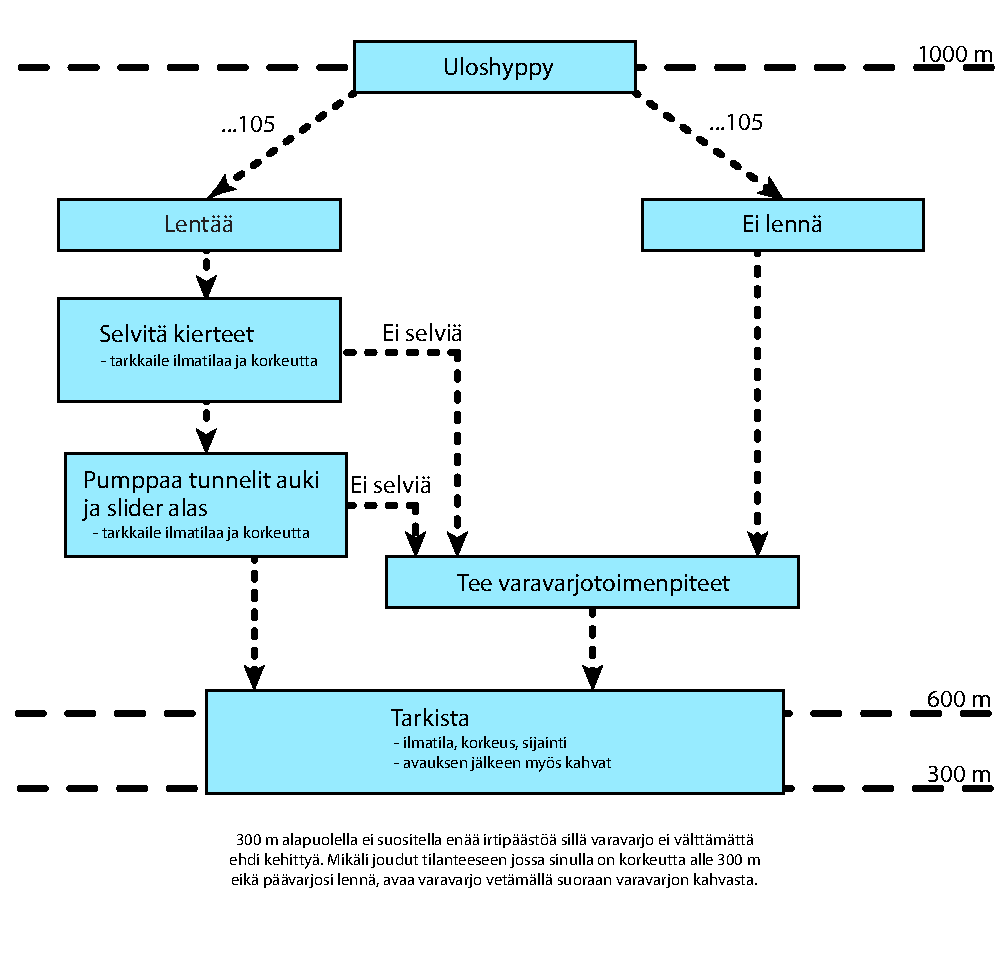
\includegraphics[width=0.99\textwidth]{VVkaavio.pdf}\caption{Toiminta päävarjon vajaatoiminnoissa}\end{figure*} 

\end{multicols}

\chapter{Mahdolliset vaaratilanteet}
\label{mahdolliset-vaaratilanteet}
\thispagestyle{headings}
\begin{multicols}{2}
\section{ Vaaratilanteet koneessa ja uloshypyssä }
\label{mahdolliset-vaaratilanteet-vaaratilanteet-koneessa-ja-uloshypyssa}

\subsection{ Repun aukeaminen koneessa }
\label{mahdolliset-vaaratilanteet-repun-aukeaminen-koneessa}


Repun (pää- tai varavarjon) tahaton aukeaminen johtuu yleensä hyppääjän varomattomasta liikkumisesta. Reppu, varavarjon kahva tai päävarjon aukaisujärjestelmä voivat tarttua jonnekin kiinni. Rauhallinen, tarpeettomia liikkeitä välttävä liikkuminen ehkäisee tarttumistilanteita tehokkaasti. Jos oma tai jonkun muun reppu kuitenkin aukeaa, estetään varjon avautuminen sekä ilmoitetaan asiasta hyppymestarille. 


Koneen lentäessä ovi auki on mahdollista, että reppu aukeaa ja varjo joutuu ilmavirtaan. Jos varjo purkautuu koneen sisällä ja ilmavirta tarttuu siihen, varjo voi vetää hyppääjän ulos. Tällaisessa tilanteessa sekä lentokone että hyppääjä voivat vahingoittua.  


Jos reppusi aukeaa ovella ja varjo karkaa ovesta ulos, hyppää ulos asennosta välittämättä. Tällaisessa tapauksessa hyppymestari auttaa sinut ripeästi ulos. Nopealla toiminnalla tilanne voidaan pelastaa. 

\subsection{ Hätähyppy }
\label{mahdolliset-vaaratilanteet-hatahyppy}


Jos lentäjän täytyy keventää konetta tai kone on ohjauskyvytön, hyppymestari antaa hyppääjille komennon HÄTÄHYPPY!  Komennolla OVELLE! siirrytään etuilematta ovelle ja komennolla MENE! poistutaan välittömästi. Hätähyppyä jatketaan, kunnes kaikki ovat hypänneet tai hyppymestari komentaa SEIS, PAKKOLASKU! Tällöin loput koneessa olevat valmistautuvat pakkolaskuun. 

\subsection{ Pakkolasku }
\label{mahdolliset-vaaratilanteet-pakkolasku}


Hyppytoiminnassa lennetään yleensä niin lähellä kenttää, että hyppykone pystyy liitämään takaisin esimerkiksi moottorihäiriön sattuessa. Tällöin hyppymestari ilmoittaa asiasta komennolla PAKKOLASKU! Automaattilaukaisin käännetään tällöin OFF-asentoon ja toimitaan ohjeiden mukaan. 


Kun kone on maassa ja pysähtynyt, on tulipalovaaran takia poistuttava nopeasti. Loukkaantuneita autetaan mahdollisuuksien mukaan. Hätähypyssä ja pakkolaskussa on muistettava, että lentäjä on koneen päällikkö mutta hyppääjien johtaja on hyppymestari. Oppilaille ohjeet tulevat \textbf{aina} hyppymestarilta. Tärkeintä on toimia rauhallisesti käskyjen mukaan. 

\subsection{ Koneeseen kiinni jääminen }
\label{mahdolliset-vaaratilanteet-koneeseen-kiinni-jaaminen}


Jos jäät roikkumaan koneeseen päävarjostasi, huomaat sen siitä, että roikut olkalukoista päävarjon kantohihnojen välityksellä. Yritä ottaa taivutettu asento jotta et pyöri ja voit varmistaa mistä olet kiinni. Varmistu, että olet hinauksessa vain olkalukkojen välityksellä jonka jälkeen tee varavarjotoimenpiteet. (\ref{paavarjon-vajaatoiminnot-varavarjon-kaytto} s.\pageref{paavarjon-vajaatoiminnot-varavarjon-kaytto}) 

\section{ Sotkeutuminen punoksiin }
\label{mahdolliset-vaaratilanteet-sotkeutuminen-punoksiin}


Jos uloshyppysi tai avausasentosi on huono, on mahdollista, että sotkeudut punoksiin. Pyri tällöin irrottautumaan takertuneista punoksista ennen varavarjotoimenpiteitä. Käytä tarvittaessa koukkupuukkoa. Tee kuitenkin varavarjotoimenpiteet (\ref{paavarjon-vajaatoiminnot-varavarjon-kaytto} s.\pageref{paavarjon-vajaatoiminnot-varavarjon-kaytto}) viimeistään 600 metrin korkeudessa. Punoksiin sotkeutumisen voi välttää keskittymällä hyvään asentoon ulos hypätessä ja varjoa avatessa. 

\section{ Apuvarjon aiheuttamat vaaratilanteet }
\label{mahdolliset-vaaratilanteet-apuvarjon-aiheuttamat-vaaratilanteet}


Huono avausasento voi johtaa siihen, että apuvarjon yhdyspunos kietoutuu esimerkiksi kätesi ympärille. Ravista kättäsi saadaksesi yhdyspunoksen irti. Jos et saa yhdyspunosta yhdellä yrityksellä irti tai et tiedä mihin se on tarttunut, tee varavarjotoimenpiteet. (\ref{paavarjon-vajaatoiminnot-varavarjon-kaytto} s.\pageref{paavarjon-vajaatoiminnot-varavarjon-kaytto}) Jos yhdyspunos on tarttunut käteesi, voit joutua tekemään varavarjotoimenpiteet yhdellä kädellä. Hyvällä uloshypyllä, avausasennolla sekä apuvarjon kunnollisella heittämisellä vapaaseen ilmavirtaan ehkäiset tehokkaasti edellisen kaltaisia vaaratilanteita. 


Apuvarjo voi avautumistilanteessa joskus tulla kuvun etureunan kautta kuvun alapuolelle. Tee ohjauskokeiluja saadaksesi selville käyttäytyykö varjo normaalisti. Jos varjo ei ohjaudu tai tekee rajuja liikkeitä, tee varavarjotoimenpiteet. (\ref{paavarjon-vajaatoiminnot-varavarjon-kaytto} s.\pageref{paavarjon-vajaatoiminnot-varavarjon-kaytto}) 


Avauksessa apuvarjo voi jäädä hyppääjän selän taakse muodostuvaan pyörteeseen eli turbulenssiin. Jos apuvarjon heiton jälkeen laskettuasi 105:een ei ole tapahtunut mitään, vilkaise olkapään yli (tarkasta). Asento kallistuu ja apuvarjon pitäisi saada ilmaa. Ellei varjo heti avaudu, tee varavarjotoimenpiteet, (\ref{paavarjon-vajaatoiminnot-varavarjon-kaytto} s.\pageref{paavarjon-vajaatoiminnot-varavarjon-kaytto}) koska apuvarjo tai yhdyspunos on saattanut tarttua johonkin kiinni tai reppu on jumissa. Kiinni tarttunutta osaa voidaan yrittää irrottaa, jos varmuudella nähdään ongelman aiheuttaja. Jos irrotus ei onnistu yhdellä yrityksellä tai et näe ongelman aiheuttajaa, tee varavarjotoimenpiteet heti. 

\section{ Vaaratilanteet varjon varassa }
\label{mahdolliset-vaaratilanteet-vaaratilanteet-varjon-varassa}

\subsection{ Kaksi varjoa auki }
\label{mahdolliset-vaaratilanteet-kaksi-varjoa-auki}


Yleisimmät syyt oppilailla kahden varjon varaan joutumisessa ovat matala avaus (itseaukaisuhypyillä), automaattilaukaisimen toimintahäiriö tai liian raju varjon käsittely (mm. poraaminen tai sakkaaminen). Kahden varjon tilanteissa ei lennetä laskeutumiskuviota. Mikäli toisen varjon puolijarrut ovat auki, pidä varjojen nopeus samana sopivilla jarruasetuksilla. 

%% Kahden liitovarjon yhdistelmä voi asettua erilaisiin muodostelmiin, jos molemmat varjot lentävät: 

\subsubsection{ Varjot peräkkäin (biplane) }
\label{mahdolliset-vaaratilanteet-varjot-perakkain-biplane}


Ohjaa varovasti etummaista varjoa vain välttämättömillä ohjausliikkeillä takimmaisista kantohihnoista. Älä avaa puolijarruja. Älä jarruta alastulossa ja valmistaudu kovaan alastuloon. 


\textbf{Älä päästä päävarjoa irti!} 


\begin{Figure}\centering\includegraphics[width=0.95\textwidth]{2-kupua-biplane.jpeg}\captionof{figure}{Varjot peräkkäin (biplane)}\end{Figure} 

\subsubsection{ Varjot vierekkäin (side-by-side) }
\label{mahdolliset-vaaratilanteet-varjot-vierekkain-side-by-side}


Ohjaa varovasti hallitsevaa varjoa vain välttämättömillä ohjausliikkeillä takimmaisista kantohihnoista. Älä avaa puolijarruja. Älä jarruta alastulossa ja valmistaudu kovaan alastuloon. 


\textbf{Älä päästä päävarjoa irti!}  


\begin{Figure}\centering\includegraphics[width=0.95\textwidth]{2-kupua-sidebyside.jpeg}\captionof{figure}{Varjot vierekkäin (side-by-side)}\end{Figure} 

\subsubsection{ Varjot sivuilla, vajoavat nopeasti (downplane) }
\label{mahdolliset-vaaratilanteet-varjot-sivuilla-vajoavat-nopeasti-downplane}


Tämä lentotila on harvinainen. Varjot voivat siirtyä itsestään varjot vierekkäin -muodostelmaan. 


\textbf{Päästä päävarjo irti!} 


\begin{Figure}\centering\includegraphics[width=0.95\textwidth]{2-kupua-downplane.jpeg}\captionof{figure}{Varjot sivuilla (downplane)}\end{Figure} 

\subsection{ Törmääminen varjon varassa }
\label{mahdolliset-vaaratilanteet-tormaaminen-varjon-varassa}


Törmäys on mahdollinen aina, kun ilmassa on useita hyppääjiä. Heti, kun olet tarkastanut, että varjo lentää, tarkasta ilmatila ja ole valmiina väistämään. Ennen puolijarrujen avaamista voit ohjata varjoa takimmaisista kantohihnoista (mikäli punokset eivät ole kierteellä). Väistä \textbf{oikealle!} 


Katso aina ennen käännöstä käännöksen suuntaan varmistaaksesi vapaa ilmatila. Alempana olevalla on aina etuajo-oikeus. Jos et voi välttää törmäämistä, minimoi törmäysvauhti jarruttamalla voimakkaasti sekä käperry \textit{palloksi.} Varoita toista hyppääjää huutamalla. 


Sotkeutumistilanteessa: 

\begin{itemize}
\item  Tarkkaile korkeutta, sillä päätökset on tehtävä riittävän korkealla 
\item  Keskustele aina kaverisi kanssa siitä, mitä aiotte tehdä 
\item  Varmista, että olet irti punoksista/kuvusta (käytä tarvittaessa koukkupuukkoa) ennen varavarjotoimenpiteitä. 
\end{itemize}

Jos ylempi varjo lentää ja alempi on sotkeutunut, voi alempi hyppääjä tehdä varavarjotoimenpiteet ja ylempi yleensä laskeutua päävarjollaan. Jos varjot ovat sotkeutuneet toisiinsa, joutuvat luultavasti molemmat tekemään varavarjotoimenpiteet. Tällöin molempien pitää sopia, missä järjestyksessä toimitaan, jotta vältetään törmääminen varavarjojen varassa. Jos korkeutta on liian vähän varavarjotoimenpiteisiin (alle 300 m), voi kaksikin ihmistä laskeutua yhdellä varjolla. 


Huomioi kaikissa toimenpiteissäsi ajan ja korkeuden menetys. 

\section{ Laskeutuminen epätavallisiin paikkoihin  }
\label{mahdolliset-vaaratilanteet-laskeutuminen-epatavallisiin-paikkoihin}


Laskeutumisen muihin paikkoihin kuin maalialueelle voi yleensä välttää ohjaamalla oikein. Alussa korkeuden ja kuljettavan matkan arviointi voi olla hankalaa, mutta hyppykokemuksen karttuessa tämäkin taito kehittyy. Joskus uloshyppypaikka voi olla väärä. Näin voi käydä etenkin, jos tuulet ovat yllättäen muuttuneet. Oli syy väärään uloshyppypaikkaan mikä tahansa, ajoissa tehty varalaskusuunnitelma mahdollistaa turvallisen laskeutumisen myös maalialueen ulkopuolelle. Suunnitelman muuttaminen viime hetkellä on vaarallista! 


Hyviä varalaskupaikkoja ovat esimerkiksi pellot ja muut aukeat alueet. Riippumatta siitä, mihin laskeudut, pyri aina laskeutumaan vastatuuleen! Pääasia on kuitenkin, että et tee jyrkkiä käännöksiä matalalla. Muista aina ottaa hyvä alastuloasento ja pitää se tiukasti maahan asti. 


Maalialueen ulkopuolelle laskeutuessasi et välttämättä enää loppuvaiheessa näe tuulipussia. Paina siksi mieleesi jo hypylle lähtiessäsi esimerkiksi se, missä suunnassa aurinko on, kun olet kääntynyt vastatuuleen. Liput, viirit ja savut ovat myös hyviä tuulen suunnan osoittimia. 

\subsection{ Laskeutuminen veteen }
\label{mahdolliset-vaaratilanteet-laskeutuminen-veteen}


Laskeudu mieluummin metsään kuin veteen. Joutuessasi laskeutumaan veteen pyri niin lähelle rantaa kuin mahdollista. Veteen laskeutuessasi toimi seuraavasti: 

\begin{itemize}
\item  Vapauta varavarjon pakkolaukaisuhihna 
\item  Käännä FXC OFF-asentoon 
\item  Löysää rintahihna 
\item  Ota alastuloasento 
\item  Tee loppuveto ennen veteen tuloa. 
\end{itemize}

Vedessä: 

\begin{itemize}
\item  Tukahduta varjo tarvittaessa tekemällä päävarjon irtipäästö 
\item  Avaa hihnat ja ui eroon varjosta. 
\end{itemize}
\subsection{ Laskeutuminen puuhun/metsään }
\label{mahdolliset-vaaratilanteet-laskeutuminen-puuhun-metsaan}


Puuhun tai metsään laskeutuessasi toimi seuraavasti: 

\begin{itemize}
\item  Vältä yksittäisiä ja korkeita puita 
\item  Ota alastuloasento ja vedä polvet ylös suojaamaan alavartaloa 
\item  Tee loppuveto puiden latvoihin sekä pidä kyynärpäät kyljissä kiinni 
\item  Valmistaudu tulemaan maahan asti ja pura alastuloasento vasta, kun liike loppuu. 
\end{itemize}

Jos jäät puuhun roikkumaan, älä pudottaudu korkealta, vaan odota apua. 


Suuri vaakanopeus aiheuttaa enemmän kolhuja kuin suuri vajoamisnopeus. Loppuvedon tekeminen puiden latvoihin on turvallisempaa kuin puita päin lentäminen. 

\subsection{ Laskeutuminen sähkölinjoihin }
\label{mahdolliset-vaaratilanteet-laskeutuminen-sahkolinjoihin}


Jos joudut laskeutumaan sähkölinjoihin, niin 

\begin{itemize}
\item  Heitä mahdollisesti käsissäsi olevat kahvat pois 
\item  Ohjaa varjoa loppuun saakka 
\item  Ota alastuloasento ja tee loppuveto linjoihin 
\item  Estä johtimien meno jalkojen väliin tai kainaloihin 
\item  Jos varjo jää kiinni, \textbf{älä yritä irrottaa sitä} 
\item  Odota apua. 
\end{itemize}
\subsection{ Laskeutuminen katolle }
\label{mahdolliset-vaaratilanteet-laskeutuminen-katolle}


Mikäli joudut laskeutumaan katolle, toimi seuraavasti: 

\begin{itemize}
\item  Ota alastuloasento 
\item  Tee loppuveto katolle 
\item  Tukahduta varjo välittömästi ja tee tarvittaessa päävarjon irtipäästö 
\item  Tartu kiinni kattorakenteista 
\item  Odota apua. 
\end{itemize}
\subsection{ Kiinteään esteeseen törmääminen }
\label{mahdolliset-vaaratilanteet-kiinteaan-esteeseen-tormaaminen}


Näitä ovat esimerkiksi seinät, autot, pylväät ja aidat. Jos osut kiinteään esteeseen, 

\begin{itemize}
\item  Tee loppuveto ennen törmäystä 
\item  Ota isku vastaan jaloilla 
\item  Valmistaudu maahantuloon 
\end{itemize}

Hyvän alastuloasennon merkitys korostuu, jos joudut laskeutumaan muualle kuin maalialueelle. 

\end{multicols}

\chapter{NOVA-Alkeiskoulutuksen suoritukset}
\label{nova-alkeiskoulutuksen-suoritukset}
\thispagestyle{headings}
\begin{multicols}{2}

NOVA-koulutusohjelmassa oppilaalle annetaan henkilökohtaista koulutusta. Tasokoulutus koostuu seitsemästä erilaisesta tasosta. Jokaisella tasohypyllä on mukana vähintään yksi novahyppymestari. Tasokoulutuksessa edetään omaa tahtia. Jokaisella hypyllä hyödynnetään edellisten tasojen osaamista, joten oppilaan on suoritettava kukin taso hyväksytysti ennen etenemistä. 


Oppilaan on saavutettava välttämättömät oppimistavoitteet hyväksytysti päästäkseen seuraavalle tasolle. Jos ensimmäisen hypyn koulutuksesta on kulunut jonkin aikaa eikä sitä jostain syystä ole hypätty, koulutus on annettava uudelleen.  

\section{ Vapaapudotus NOVA-hypyillä }
\label{nova-alkeiskoulutuksen-suoritukset-vapaapudotus-nova-hypyilla}


Ulos hypätessä taivuta lantiosta, siirrä kädet ja jalat oikeaan asentoon ja pidä katse koneessa niin kauan kuin mahdollista. Pyri rentoutumaan puhaltamalla ulos hengittäessä suun kautta ja pidä leuka ylhäällä. Kuvittele puskevasi lantiota ilman halki. 

\subsection{Tarkkailukehä}
\label{nova-alkeiskoulutuksen-suoritukset-tarkkailukeha}


Laskettuasi 105:een aloita ja suorita omatoimisesti tarkkailukehä: 

\begin{enumerate}[label=\bfseries \arabic*)]
\item  MAA 
	\begin{itemize}
	\item  Siirrä katseesi 45° kulmassa alaspäin ja valitse jokin iso ja helposti löydettävä kiintopiste 
	\end{itemize}
\item  MITTARI 
	\begin{itemize}
	\item  Pidä taivutus, siirrä katseesi mittariin ja lue lukema. 
	\end{itemize}
\item  KORKEUS (VV-HM, varavarjon puoleinen hyppymestari) 
	\begin{itemize}
	\item  Katso vasemmalla puolella olevaa hyppymestaria käsivarren alta ja sano hänelle korkeusmittarin lukema. Hyppymestari voi tässä vaiheessa korjata asentoasi käsimerkein. Jos asennossa ei ole mitään korjattavaa, saat OK-käsimerkin (peukalo ylös). Älä jatka tarkkailukehää ennen kuin olet saanut OK-käsimerkin! 
	\end{itemize}
\item  KORKEUS (PV-HM, päävarjon puoleinen hyppymestari) 
	\begin{itemize}
	\item  Katso oikealla puolella olevaa hyppymestaria käsivarren alta ja suorita sama toimenpide kuin edellä. Jos kaikki on kunnossa saat OK-käsimerkin. Älä jatka tarkkailukehää ennen kuin olet saanut OK-käsimerkin! 
	\end{itemize}
\end{enumerate}

Tarkkailukehän avulla säilytät tietoisuuden korkeudesta ja suunnasta.  

\subsection{Harjoitusveto}
\label{nova-alkeiskoulutuksen-suoritukset-harjoitusveto}


Aloita itsenäisesti, mutta jos näet harjoitusveto-käsimerkin, se merkitsee harjoitusvedon aloittamista. Toimi rytmikkäästi ja sano toimenpiteet ääneen. 

\begin{enumerate}[label=\bfseries \arabic*)]
\item  TAIVUTA 
	\begin{itemize}
	\item  Työnnä lantiota alaspäin / varmista taivutus. 
	\item  Taivutus säilyy ja leuka pysyy ylhäällä koko harjoitusvedon ajan. 
	\end{itemize}
\item  TARTU 
	\begin{itemize}
	\item  Pidä katse ylhäällä. Siirrä vasen käsi pääsi yläpuolelle siten, että peukalo koskettaa päätäsi (otsaa) kämmenen ollessa auki. Siirrä oikea kätesi päävarjon avauskahvalle kämmen auki. Käsien liikkeiden on tapahduttava symmetrisesti, samalla tasolla ja yhdenaikaisesti. Vain kädet liikkuvat. Pään tai muun vartalon asento ei muutu.  
	\item  Kosketa kahvaa ja paina mieleesi kahvan paikka. On tärkeää tuntea selvästi, missä se on.   
	\end{itemize}
\item  VEDÄ 
	\begin{itemize}
	\item  Palauta kädet alkuperäiseen asentoon symmetrisesti ja yhdenaikaisesti. Vain kädet liikkuvat. Pään tai muun vartalon asento ei muutu. Huom! Kyseessä on harjoitusveto, joten älä vedä oikeasti. 
	\end{itemize}
\end{enumerate}
\subsection{ Varjon avaus }
\label{nova-alkeiskoulutuksen-suoritukset-varjon-avaus}


Ensimmäisellä hypylläsi aloitat avaustoimenpiteet 1600 metrin korkeudessa. Näytä ensin avausmerkki, jolla ilmoitat muille avaavasi varjosi, eli heilauta käsiäsi ristiin pääsi edessä. Avausmerkin jälkeen aloitat rauhallisesti ja täsmällisesti avaustoimenpiteet. Avaus tehdään samalla tavalla kuin harjoitusveto. Erona on vain se, että apuvarjon kahvasta tartutaan kunnolla kiinni ja apuvarjo heitetään reippaasti ilmavirtaan. Varjon ei siis pidä olla auki heti 1600 metrissä.  


TAIVUTA - TARTU - VEDÄ 


Tämän jälkeen laske ääneen 101, 102…105, jonka jälkeen tarkistat varjon ja suoritat mahdolliset selvitystoimenpiteet. Mikäli varjo ei selviä tai ei lennä, tee varavarjotoimenpiteet. Tasoilla 1-2 VV-HM pitää sinusta kiinni varjon avautumiseen asti ja tasoilla 3-7 HM varmistaa avautumisen.  

\section{ Taso 1 - Tottuminen vapaapudotukseen }
\label{nova-alkeiskoulutuksen-suoritukset-taso-1-tottuminen-vapaapudotukseen}


Kaksi novahyppymestaria, kolmella ensimmäisellä hypyllä radio. 


Jos näet vain yhden hyppymestarin, seuraa hänen ohjeitaan ja jatka hyppysuoritusta normaalisti ohjelman mukaan. Tasoilla 1 ja 2 \textbf{et} saa olla yksin vapaapudotuksessa. Jos et näe kumpaakaan hyppymestaria, avaa varjo välittömästi eli TAIVUTA-TARTU-VEDÄ 101..105 ja tarkista varjo.  

\subsection{ Oppilaan toiminta. }
\label{nova-alkeiskoulutuksen-suoritukset-oppilaan-toiminta}


Harjoittele 1. tason kulku (ja myöhemmin kaikki muut tasot) mahdollisimman hyvin etukäteen, sillä se helpottaa ja nopeuttaa huomattavasti oppimistasi. 

\subsection{ Ensimmäiseen hyppyysi valmistautuminen }
\label{nova-alkeiskoulutuksen-suoritukset-ensimmaiseen-hyppyysi-valmistautuminen}

\begin{enumerate}[label=\bfseries \arabic*)]
\item  Näytä, miten koneen ovelle siirrytään hyppyasentoon. 
\item  Esitä oikea hallittu uloshyppy mukaan lukien laskeminen. 
\item  Käy läpi ja harjoittele suunniteltu hyppy kohta kohdalta. 
\item  Harjoittele harjoitusvetoa samalla tavalla kuin oikeaa avausliikettä. 
	\begin{itemize}
	\item  a. TAIVUTA taivutus säilyy. Katse eteenpäin leuka ylhäällä. 
	\item  b. TARTU säilytä taivutus, kun siirrät samanaikaisesti oikean käden kämmen auki päävarjon avauskahvalle ja siirrä vasen käsi pääsi yläpuolelle siten, että peukalo koskettaa päätäsi (otsaa) kämmen avattuna. Paina tarkasti mieleesi kahvan paikka. Molemmat kädet pysyvät samassa tasossa. Vain kädet liikkuvat, ei pää eikä muu vartalon osa. Katse eteenpäin leuka ylhäällä. 
	\item  c. VEDÄ palauta kädet alkuperäiseen asentoon symmetrisesti sekä yhdenaikaisesti, katse eteenpäin ja leuka ylhäällä. Vain kädet liikkuvat, pään tai muun vartalon asento ei muutu lainkaan. HUOM. Tämä on harjoitusveto, joten älä vedä oikeasti.  
	\end{itemize}
\item  Harjoittele toimenpiteitä lennon ja hypyn aikana sattuvien vaaratilanteiden varalta. 
\item  Katso maatuulen suunta tuulipussista ja kuvaile oikeat ohjauskuviot. 
\item  Näytä oikea alastulo- ja kaatumisasento. 
\item  Kertaa käsimerkit. 
\end{enumerate}
\subsection{ Oppimistavoitteet }
\label{nova-alkeiskoulutuksen-suoritukset-oppimistavoitteet}


Jokaisella tasolla on omat oppimistavoitteet, joiden mukaan arvioidaan oppimisesi, sekä se, pääsetkö seuraavalle tasolle. Tutustu oppimistavoitteisiin tarkasti HM:n kanssa. 

\begin{enumerate}[label=\bfseries \arabic*)]
\item  Stabiilin vapaapudotusasennon löytäminen viimeistään 10 sekuntia ennen avauskorkeutta 
\item  Korkeuden tarkkailu 
\item  Avausmerkki 1600 m (±300m) ja avaus 
\end{enumerate}
\subsection{ Hyppylennolla }
\label{nova-alkeiskoulutuksen-suoritukset-hyppylennolla}

\begin{itemize}
\item  Katso laskeutumisalue ja oikea laskeutumissuunta yli 600 m:n korkeudessa. Hyppymestari kysyy tärkeitä korkeuksia. 
\item  Hyppymestari kysyy hypyn avainkohdat. 
\end{itemize}
\subsection{ Hypyn kulku }
\label{nova-alkeiskoulutuksen-suoritukset-hypyn-kulku}

\begin{tabular}[]{|l|p{4.7cm}|}
\hline
 \textbf{2700-4000 m} &  Rento taivutettu UH
\\ \hline
  &  Tarkkailukehä
\\ \hline
  &  3 Harjoitusvetoa
\\ \hline
  &  Tarkkailukehä
\\ \hline
  &  MAA - MITTARI
\\ \hline
 \textbf{1600 m} &  Avausmerkki ja avaus
\\ \hline
\end{tabular}

\end{multicols}\pagebreak\begin{multicols}{2} 

\section{ Taso 2 - Asennon hallinta }
\label{nova-alkeiskoulutuksen-suoritukset-taso-2-asennon-hallinta}


Kaksi novahyppymestaria, kolmella ensimmäisellä hypyllä radio.   Oppilaan on saavutettava välttämättömät oppimistavoitteet hyväksytysti päästäkseen seuraavalle tasolle. 

\subsection{ Oppilaan toiminta. }
\label{nova-alkeiskoulutuksen-suoritukset-oppilaan-toiminta}

\begin{enumerate}[label=\bfseries \arabic*)]
\item  Käy läpi I-tasolla opitut tiedot ja taidot. 
\item  Harjoittele stabiilia asentoa esim. rullalaudoilla. 
\item  Harjoittele kaikkia vapaassa tehtäviä liikkeitä kuten aikaisemmilla tunneilla. 
\item  Harjoittele harjoitusvetoa kuten oikeaa avausta. 
\item  Näytä maalialue ja käy läpi ennalta suunniteltu ohjauskuvio. 
\item  Käytä mielikuvaharjoittelua valmistautuessasi hyppyyn. 
\item  Osallistu itse aikaisempaa enemmän varusteiden tarkistukseen ja sovittamiseen. 
\end{enumerate}
\subsection{ Oppimistavoitteet }
\label{nova-alkeiskoulutuksen-suoritukset-oppimistavoitteet}

\begin{enumerate}[label=\bfseries \arabic*)]
\item  Stabiili vapaapudotusasento viimeistään 10 sekuntia UH:n jälkeen 
\item  Stabiilin vapaapudotusasennon säilyttäminen koko hypyn ajan, sisältäen jalkojen hallinnan 
\item  Avausmerkki 1600 m (±150 m) ja itsenäinen avaus  
\item  Itsenäisempi, turvallinen varjon ohjailu 
\end{enumerate}
\subsection{ Hyppylennolla }
\label{nova-alkeiskoulutuksen-suoritukset-hyppylennolla}

\begin{enumerate}[label=\bfseries \arabic*)]
\item  Toista kaikki aikaisemmin opetetut toimenpiteet lennon aikana. 
\item  Käytä rentouttavaa hengitystekniikkaa (hengitä hitaasti sisään, pidätä hetkisen ja rentoudu uloshengittäessäsi). 
\item  Näytä maamerkkejä ja osoita avauskorkeus hyppymestareille. 
\end{enumerate}
\subsection{ Hypyn kulku }
\label{nova-alkeiskoulutuksen-suoritukset-hypyn-kulku}

\begin{tabular}[]{|l|p{4.7cm}|}
\hline
 \textbf{2700-4000 m} &  Rento, taivutettu uloshyppy
\\ \hline
  &  Tarkkailukehä
\\ \hline
  &  Harjoitusvetoja kunnes OK
\\ \hline
  &  MAA, MITTARI, TAIVUTA, JALAT, RENTOUTA
\\ \hline
  &  Liike eteenpäin
\\ \hline
  &  MAA, MITTARI, TAIVUTA, JALAT, RENTOUTA
\\ \hline
  &  90° vasen
\\ \hline
  &  MAA, MITTARI, TAIVUTA, JALAT, RENTOUTA
\\ \hline
  &  90° oikea
\\ \hline
  &  MAA, MITTARI, TAIVUTA, JALAT, RENTOUTA
\\ \hline
 \textbf{1600 m} &  Avausmerkki ja avaus
\\ \hline
\end{tabular}

\end{multicols}\pagebreak\begin{multicols}{2} 

\section{ Taso 3 - Stabiili vapaapudotus }
\label{nova-alkeiskoulutuksen-suoritukset-taso-3-stabiili-vapaapudotus}


Kaksi novahyppymestaria, kolmella ensimmäisellä hypyllä radio. 


Oppilaan on saavutettava välttämättömät oppimistavoitteet hyväksytysti päästäkseen seuraavalle tasolle. 


Jos tasoilla 3-7 et näe kumpaakaan hyppymestaria, voit jatkaa hyppyä, mikäli kaikki alla olevat ehdot täyttyvät: 

\begin{itemize}
\item  Tiedät korkeutesi  
\item  Et pyöri mihinkään suuntaan 
\item  Et ole selälläsi 
\item  Tilanne tuntuu kaiken kaikkiaan olevan hallinnassa 
\end{itemize}

Tarkkaile korkeutta koko ajan n. 5 s välein (MAA, MITTARI, TAIVUTA, JALAT, RENTOUTA) ja tason mukaisessa korkeudessa tee avausmerkki ja avaa päävarjo normaalisti. Älä tee muita suorituksia.  


Jos et avauksessa löydä päävarjon kahvaa, yritä toisen kerran, mutta jos et \textbf{heti} löydä kahvaa, tee varavarjotoimenpiteet. 


Jos et avauksessa jaksa vetää päävarjon kahvasta (tiukka kahva), yritä toisen kerran, mutta jos et silloinkaan \textbf{heti} saa varjoa auki, tee varavarjotoimenpiteet. 

\subsection{ Oppilaan toiminta. }
\label{nova-alkeiskoulutuksen-suoritukset-oppilaan-toiminta}

\begin{enumerate}[label=\bfseries \arabic*)]
\item  Kuvaile ja esitä käytännössä tiedot ja taidot, jotka on opittu aikaisempien hyppyjen yhteydessä. 
\item  Harjoitteleilmatilan tarkistusta HM:n avustuksella. 
\item  Harjoittele maassa tekniikkaa jolla käännyt tarvittaessa selältään oikein päin. 
\item  Näytä millä tekniikalla suunta säilytetään vapaapudotuksessa. 
\item  Keskity hyppyyn ja rentoudu. Mieti, millainen on hyvä stabiili asento ja harjoittele sitä. 
\item  Käy läpi hypyn kulku ja harjoittele sitä käytännössä. 
\end{enumerate}
\subsection{ Oppimistavoitteet }
\label{nova-alkeiskoulutuksen-suoritukset-oppimistavoitteet}

\begin{enumerate}[label=\bfseries \arabic*)]
\item  Ilmatilan tarkistus ennen uloshyppyä 
\item  Stabiili itsenäinen vapaapudotus viimeistään 5 sekuntia UH:n jälkeen 
\item  Tarkoituksettomien käännösten pysäyttäminen 
\item  Avausmerkki 1600 m (±150m), stabiili itsenäinen avustamaton avaus ilman NHM:n otetta oppilaasta 
\item  Itsenäinen, turvallinen varjon ohjailu 
\end{enumerate}
\subsection{ Hyppylennolla }
\label{nova-alkeiskoulutuksen-suoritukset-hyppylennolla}

\begin{enumerate}[label=\bfseries \arabic*)]
\item  Toista aiemmin opitut toimenpiteet. 
\item  Käytä rentouttavaa hengitystekniikkaa ja positiivisia mielikuvia. 
\item  Katso HM:n johdolla lentokenttää ja ilmatilaa ovella ennen uloshyppyä. 
\end{enumerate}
\subsection{ Ohjailu ja laskeutuminen }
\label{nova-alkeiskoulutuksen-suoritukset-ohjailu-ja-laskeutuminen}

\begin{enumerate}[label=\bfseries \arabic*)]
\item  Toimi kuten edellisillä hypyillä, mutta tee kaikki entistä tarkemmin. 
\item  Seisontalaskua saa yrittää (mutta pidä aina hyvä alastuloasento). 
\end{enumerate}
\subsection{ Hypyn kulku }
\label{nova-alkeiskoulutuksen-suoritukset-hypyn-kulku}

\begin{tabular}[]{|l|p{4.7cm}|}
\hline
 \textbf{2700-4000 m} &  Rento taivutettu UH
\\ \hline
  &  Tarkkailukehä
\\ \hline
  &  Harjoitusvetoja kunnes OK
\\ \hline
  &  Stabiili itsenäinen vapaapudotus
\\ \hline
  &  MAA, MITTARI, TAIVUTA, JALAT, RENTOUTA
\\ \hline
 \textbf{1600 m} &  Avausmerkki ja avaus
\\ \hline
\end{tabular}

\end{multicols}\pagebreak\begin{multicols}{2} 

\section{ Taso 4 - Käännökset 90° }
\label{nova-alkeiskoulutuksen-suoritukset-taso-4-kaannokset-90deg}


Yksi novahyppymestari. 


Oppilaan on saavutettava välttämättömät oppimistavoitteet hyväksytysti päästäkseen seuraavalle tasolle. 

\subsection{ Oppilaan toiminta. }
\label{nova-alkeiskoulutuksen-suoritukset-oppilaan-toiminta}

\begin{enumerate}[label=\bfseries \arabic*)]
\item  Osaat tehdä varusteiden tarkastuksen maassa ja ennen koneelle menoa. (\ref{laskuvarjokalusto-ja-hyppyvarusteet-3x3-tarkastus} s.\pageref{laskuvarjokalusto-ja-hyppyvarusteet-3x3-tarkastus}) 
\item  Harjoittele koko hyppytapahtuman kulku käytännössä. 
\item  Tarkista ilmatila ja pilvet ennen uloshyppyä ja huomioi riittävä exit-väli edelliseen ryhmään. 
\item  Tarkista varusteet ennen UH:ta (\ref{laskuvarjokalusto-ja-hyppyvarusteet-3x3-tarkastus} s.\pageref{laskuvarjokalusto-ja-hyppyvarusteet-3x3-tarkastus}) 
\end{enumerate}
\subsection{ Oppimistavoitteet }
\label{nova-alkeiskoulutuksen-suoritukset-oppimistavoitteet}

\begin{enumerate}[label=\bfseries \arabic*)]
\item  Ilmatilan ja pilvien tarkistus ja exit-väli  
\item  Omien varusteiden tarkastus (maassa ja koneessa) 
\item  Stabiili vapaapudotusasento 
\item  Vähintään kaksi hallittua 90° käännöstä (±20°) 
\item  Avausmerkki 1500 m (±150 m), stabiili itsenäinen avustamaton avaus  
\end{enumerate}
\subsection{ Hyppylennolla }
\label{nova-alkeiskoulutuksen-suoritukset-hyppylennolla}

\begin{enumerate}[label=\bfseries \arabic*)]
\item  Toimi lennon aikana aikaisemmin opetettujen toimenpiteiden mukaisesti. 
\item  Tarkista ilmatila ja pilvet sekä huomioi riittävä exit-väli edelliseen ryhmään. 
\end{enumerate}
\subsection{ Ohjailu ja laskeutuminen }
\label{nova-alkeiskoulutuksen-suoritukset-ohjailu-ja-laskeutuminen}

\begin{enumerate}[label=\bfseries \arabic*)]
\item  Toimi aiemmin opitulla tavalla. 
\item  Pyri laskeutumaan korkeintaan 50 m päähän kohteesta mahdollisimman vähin ohjein. 
\end{enumerate}
\subsection{ Hypyn kulku }
\label{nova-alkeiskoulutuksen-suoritukset-hypyn-kulku}

\begin{tabular}[]{|l|p{4.7cm}|}
\hline
 \textbf{2700-4000 m} &  Rento taivutettu UH
\\ \hline
  &  Tarkkailukehä (HM siirtyy oppilaan eteen)
\\ \hline
  &  Lupa käännökseen (oppilas nyökkää HM:lle, HM vastaa nyökkäämällä)
\\ \hline
  &  90° vasen
\\ \hline
  &  MAA, MITTARI, TAIVUTA, JALAT, RENTOUTA
\\ \hline
  &  90° oikea
\\ \hline
  &  MAA, MITTARI, TAIVUTA, JALAT, RENTOUTA
\\ \hline
 \textbf{2000 m} &  Ei käännöksiä
\\ \hline
  &  MAA, MITTARI, TAIVUTA, JALAT, RENTOUTA
\\ \hline
 \textbf{1500 m} &  Avausmerkki ja avaus
\\ \hline
\end{tabular}

\end{multicols}\pagebreak\begin{multicols}{2} 

\section{ Taso 5 - Käännökset 360° }
\label{nova-alkeiskoulutuksen-suoritukset-taso-5-kaannokset-360deg}


Yksi novahyppymestari. 


Oppilaan on saavutettava välttämättömät oppimistavoitteet hyväksytysti päästäkseen seuraavalle tasolle. 

\subsection{ Oppilaan toiminta. }
\label{nova-alkeiskoulutuksen-suoritukset-oppilaan-toiminta}

\begin{enumerate}[label=\bfseries \arabic*)]
\item  Näytä, että osaat oikeaoppisesti tarkastaa ja säätää varusteet. 
\item  Harjoittele koko hyppytapahtuman kulku käytännössä. 
\item  Tarkistat ilmatilan, pilvet ja huomioit exit-välin  
\item  Tarkastat automaattisesti itse varusteet ennen uloshyppyä. (\ref{laskuvarjokalusto-ja-hyppyvarusteet-3x3-tarkastus} s.\pageref{laskuvarjokalusto-ja-hyppyvarusteet-3x3-tarkastus}) 
\end{enumerate}
\subsection{ Oppimistavoitteet }
\label{nova-alkeiskoulutuksen-suoritukset-oppimistavoitteet}

\begin{enumerate}[label=\bfseries \arabic*)]
\item  Vähintään kaksi hallittua 360° käännöstä (±45°) 
\item  Yhä stabiilimpi vapaapudotus  
\item  Avausmerkki 1500 m (±150 m), stabiili suunnassa pysyvä itsenäinen avustamaton avaus   
\item  Tee varjon varassa 90° käännöksiä takimmaisista kantohihnoista puolijarrut kiinni sekä avattuina 
\end{enumerate}
\subsection{ Hyppylennolla }
\label{nova-alkeiskoulutuksen-suoritukset-hyppylennolla}

\begin{enumerate}[label=\bfseries \arabic*)]
\item  Tarkistat ilmatilan, pilvet ja huomioit exit-välin. 
\item  Tarkastat itse varusteet ennen uloshyppyä 
\end{enumerate}
\subsection{ Ohjailu ja laskeutuminen }
\label{nova-alkeiskoulutuksen-suoritukset-ohjailu-ja-laskeutuminen}

\begin{enumerate}[label=\bfseries \arabic*)]
\item  Tee 90° käännöksiä kantohihnoista puolijarrut kiinni sekä avattuina. 
\item  Pyri laskeutumaan enintään 50 metrin päähän kohteesta. 
\item  Muista oikea lähestymis- ja laskeutumistekniikka. 
\end{enumerate}
\subsection{ Hypyn kulku }
\label{nova-alkeiskoulutuksen-suoritukset-hypyn-kulku}

\begin{tabular}[]{|l|p{4.7cm}|}
\hline
 \textbf{2700-4000 m} &  Rento taivutettu UH
\\ \hline
  &  Tarkkailukehä (HM siirtyy oppilaan eteen)
\\ \hline
  &  Lupa käännökseen (oppilas nyökkää HM:lle, HM vastaa nyökkäämällä)
\\ \hline
  &  360° vasen
\\ \hline
  &  MAA, MITTARI, TAIVUTA, JALAT, RENTOUTA
\\ \hline
  &  360° oikea
\\ \hline
  &  MAA, MITTARI, TAIVUTA, JALAT, RENTOUTA
\\ \hline
 \textbf{2000 m} &  Ei käännöksiä
\\ \hline
  &  MAA, MITTARI, TAIVUTA, JALAT, RENTOUTA
\\ \hline
 \textbf{1500 m} &  Avausmerkki ja avaus
\\ \hline
\end{tabular}

\end{multicols}\pagebreak\begin{multicols}{2} 

\section{ Taso 6 - Irtiuloshyppy }
\label{nova-alkeiskoulutuksen-suoritukset-taso-6-irtiuloshyppy}


Yksi novahyppymestari. 


Oppilaan on saavutettava välttämättömät oppimistavoitteet hyväksytysti päästäkseen seuraavalle tasolle. 

\subsection{ Oppilaan toiminta. }
\label{nova-alkeiskoulutuksen-suoritukset-oppilaan-toiminta}

\begin{enumerate}[label=\bfseries \arabic*)]
\item  Toista aikaisemmilla tasoilla opitut asiat 
\item  Harjoittele suoran uloshypyn asentoa ja tekniikkaa 
\item  Harjoittele takavoltin tekniikkaa ja stabiloimista. 
\item  Delta-asento ja liukuminen. 
\end{enumerate}
\subsection{ Oppimistavoitteet }
\label{nova-alkeiskoulutuksen-suoritukset-oppimistavoitteet}

\begin{enumerate}[label=\bfseries \arabic*)]
\item  Itsenäinen, avustamaton uloshyppy 
\item  Asennon stabilointi epästabiilista viidessä sekunnissa 
\item  Liuku (suunta säilyttäen) 
\item  Avausmerkki 1300 m (±150 m) ja avaus  
\item  Oikeaoppiset lähestymis- ja laskeutumiskuviot 
\end{enumerate}
\subsection{ Hyppylennolla }
\label{nova-alkeiskoulutuksen-suoritukset-hyppylennolla}

\begin{enumerate}[label=\bfseries \arabic*)]
\item  Käy uudelleen lävitse toiminta kuten kaikilla aikaisemmilla tasoilla. 
\item  Ilmatilan tarkistus, pilvet, exit-välin huomioiminen  
\item  Tee stabiili, suora uloshyppy ilman HM:n apua 
\end{enumerate}
\subsection{ Ohjailu ja laskeutuminen }
\label{nova-alkeiskoulutuksen-suoritukset-ohjailu-ja-laskeutuminen}

\begin{enumerate}[label=\bfseries \arabic*)]
\item  Pyri laskeutumaan korkeintaan 25 m:n päähän määrätyn alastuloalueen keskustasta 
\item  Tee oikeaoppiset lähestymis- ja laskeutumiskuviot 
\end{enumerate}
\subsection{ Hypyn kulku }
\label{nova-alkeiskoulutuksen-suoritukset-hypyn-kulku}

\begin{tabular}[]{|l|p{4.7cm}|}
\hline
 \textbf{2700-4000 m} &  Suora uloshyppy 
\\ \hline
  &  MAA, MITTARI, TAIVUTA, JALAT, RENTOUTA
\\ \hline
  &  Tynnyri
\\ \hline
  &  MAA, MITTARI, TAIVUTA, JALAT, RENTOUTA
\\ \hline
  &  Takavoltti
\\ \hline
  &  MAA, MITTARI, TAIVUTA, JALAT, RENTOUTA
\\ \hline
 \textbf{Yli 2000 m} &  Lentokentän paikallistaminen ja liuku
\\ \hline
  &  MAA, MITTARI, TAIVUTA, JALAT, RENTOUTA
\\ \hline
 \textbf{1300 m} &  Avausmerkki ja avaus
\\ \hline
\end{tabular}

\end{multicols}\pagebreak\begin{multicols}{2} 

\section{ Taso 7 - Puolisarja }
\label{nova-alkeiskoulutuksen-suoritukset-taso-7-puolisarja}


Yksi novahyppymestari. 


Tämä on viimeinen tasohyppysi. Tällä tasolla sinun tulisi toimia mahdollisimman itsenäisesti ja osoittaa hallitsevasi hyppäämiseen liittyvät turvallisuustekijät, kuten stabiili vapaapudotus ja varjon avaus, sekä ohjaaminen. 

\subsection{ Oppilaan toiminta. }
\label{nova-alkeiskoulutuksen-suoritukset-oppilaan-toiminta}

\begin{enumerate}[label=\bfseries \arabic*)]
\item  Harjoittele sukellusuloshypyn asentoa ja tekniikkaa. 
\item  Harjoittele etuvoltin tekniikkaa. 
\item  Harjoittele vaakasuunnassa liikkuvaa liukua. 
\end{enumerate}
\subsection{ Oppimistavoitteet }
\label{nova-alkeiskoulutuksen-suoritukset-oppimistavoitteet}

\begin{enumerate}[label=\bfseries \arabic*)]
\item  Tarkista ilmatila, pilvet, huomioi exit-väli 
\item  Sukellusuloshyppy josta stabiili asento viidessä sekunnissa 
\item  Asennon stabilointi suoritusten aikana viidessä sekunnissa 
\item  Avausmerkki 1300 m (±150 m) ja avaus  
\item  Turvallinen varjon käsittely 
\end{enumerate}
\subsection{ Hyppylennolla }
\label{nova-alkeiskoulutuksen-suoritukset-hyppylennolla}

\begin{enumerate}[label=\bfseries \arabic*)]
\item  Tarkista ilmatila, pilvet ja huomioi exit-väli  
\item  Tarkista omat varusteesi 
\end{enumerate}
\subsection{ Ohjailu ja laskeutuminen }
\label{nova-alkeiskoulutuksen-suoritukset-ohjailu-ja-laskeutuminen}

\begin{enumerate}[label=\bfseries \arabic*)]
\item  Pyri laskeutumaan korkeintaan 25 metrin päähän määrätyn alastuloalueen keskustasta 
\item  Näytä, miten ohjaat varjoasi turvallisesti  
\end{enumerate}
\subsection{ Hypyn kulku }
\label{nova-alkeiskoulutuksen-suoritukset-hypyn-kulku}

\begin{tabular}[]{|l|p{4.7cm}|}
\hline
 \textbf{2700-4000 m} &  Sukellusuloshyppy 
\\ \hline
  &  MAA, MITTARI, TAIVUTA, JALAT, RENTOUTA
\\ \hline
  &  Etuvoltti
\\ \hline
  &  MAA, MITTARI, TAIVUTA, JALAT, RENTOUTA
\\ \hline
  &  Takavoltti
\\ \hline
  &  MAA, MITTARI, TAIVUTA, JALAT, RENTOUTA
\\ \hline
  &  360° Vasen 
/ Oikea 


\\ \hline
 \textbf{Yli 2000 m} &  Liuku
\\ \hline
  &  MAA, MITTARI, TAIVUTA, JALAT, RENTOUTA
\\ \hline
 \textbf{1300 m} &  Avausmerkki ja avaus
\\ \hline
\end{tabular}

\end{multicols}\pagebreak\begin{multicols}{2} 

\section{ 15'' - Lyhyt vapaa }
\label{nova-alkeiskoulutuksen-suoritukset-15-lyhyt-vapaa}


Yksi novahyppymestari koneessa. 


Tämä on alkeiskoulutuksen viimeinen  hyppy ja ensimmäinen hyppysi matalammasta hyppykorkeudesta. Hyppymestari ei enää hyppää mukanasi. 

\subsection{ Oppilaan toiminta. }
\label{nova-alkeiskoulutuksen-suoritukset-oppilaan-toiminta}


Toista tasokoulutuksessa oppimasi asiat: irtiuloshyppy eli suora uloshyppy, asennon stabilointi uloshypyn jälkeen, korkeuden tarkkailu ja stabiili avaus. 

\subsection{ Oppimistavoitteet }
\label{nova-alkeiskoulutuksen-suoritukset-oppimistavoitteet}

\begin{enumerate}[label=\bfseries \arabic*)]
\item  Tarkista ilmatila, pilvet ja huomioi exit-väli  
\item  Suora uloshyppy 
\item  15'' vapaapudotus koko ajan korkeutta tarkkaillen 
\item  Avausmerkki 1200 m ja avaus 
\end{enumerate}
\subsection{ Hyppylennolla }
\label{nova-alkeiskoulutuksen-suoritukset-hyppylennolla}

\begin{enumerate}[label=\bfseries \arabic*)]
\item  Tarkista omat varusteesi 
\item  Tarkista ilmatila, pilvet ja huomioi exit-väli  
\end{enumerate}
\subsection{ Ohjailu ja laskeutuminen }
\label{nova-alkeiskoulutuksen-suoritukset-ohjailu-ja-laskeutuminen}

\begin{enumerate}[label=\bfseries \arabic*)]
\item  Pyri laskeutumaan korkeintaan 25 metrin päähän määrätyn alastuloalueen keskustasta 
\item  Näytä, miten ohjaat varjoasi turvallisesti  
\end{enumerate}
\subsection{ Hypyn kulku }
\label{nova-alkeiskoulutuksen-suoritukset-hypyn-kulku}

\begin{tabular}[]{|l|p{4.7cm}|}
\hline
 \textbf{1800-2500 m} &  Suora uloshyppy
\\ \hline
  &  Mittari
\\ \hline
 \textbf{1200 m} &  Avausmerkki ja avaus
\\ \hline
\end{tabular}
\end{multicols}

\chapter{PL-Alkeiskoulutuksen suoritukset}
\label{pl-alkeiskoulutuksen-suoritukset}
\thispagestyle{headings}
\begin{multicols}{2}
\section{ Pakkolaukaisu }
\label{pl-alkeiskoulutuksen-suoritukset-pakkolaukaisu}


Ensimmäiset hyppysi ovat pakkolaukaisuhyppyjä. Irtautuessasi koneesta pakkolaukaisujärjestelmä avaa päävarjon repun ja vetää sisäpussin ulos repusta. 

\subsection{ Oppilaan toiminta }
\label{pl-alkeiskoulutuksen-suoritukset-oppilaan-toiminta}


Uloshyppyasennon tulee olla symmetrinen X-asento tai delta-asento (riippuen konetyypistä), taivutus tulee olla riittävä ja asennon tulee säilyä aina laskuvarjon aukeamiseen saakka. Vapaapudotusta ei ehdi kertyä vielä pakkolaukaisuhypyillä, mutta raajojen ja kehon asennolla on silti vaikutusta hypyn onnistumiseen. 

\subsection{ Ensimmäiseen hyppyysi valmistautuminen }
\label{pl-alkeiskoulutuksen-suoritukset-ensimmaiseen-hyppyysi-valmistautuminen}


Hyppytapahtuma ei suinkaan ala siitä, kun poistutaan koneesta ilmassa. Jotta kaikki sujuisi hyvin, on tärkeää huolehtia myös valmisteluista. Valmistaudu hyppyyn sekä henkisesti että fyysisesti: riittävä yöuni ja ravinto ovat tärkeitä. Väsyneenä tai nälkäisenä keskittyminen on vaikeaa. Ennen hyppäämään kirjoittautumista (pokalistan täyttöä) kootaan kaikki tarvittavat varusteet ja ilmoittaudutaan hyppäämään. Varusteita on hyvä sovittaa päälle, jotta niihin voi tehdä tarvittavat säädöt ajoissa ennen koneelle lähtöä. Suoritusta harjoitellaan joko itsenäisesti tai hyppymestarin kanssa. 


Mikäli mahdollista, seuraa ennen omaa pokaasi toisten hyppääjien ohjailua varjon varassa nähdäksesi ylä- ja pintatuulien vaikutuksen ohjaamiseen ja laskeutumiseen. 


Ennen koneelle menoa hyppymestari tarkastaa, että varusteet on puettu oikein päälle. Tarkastuksen jälkeen varusteita ei saa säätää ilman hyppymestarin lupaa. Vallitsevan tuulen mukainen ohjauskuvio käydään vielä läpi ennen koneelle menoa. Oppilaat saavat mennä koneelle vain hyppymestarin johdolla. 

\subsection{ Oppimistavoitteet }
\label{pl-alkeiskoulutuksen-suoritukset-oppimistavoitteet}


Oppilaan on saavutettava välttämättömät oppimistavoitteet hyväksytysti jotta hyppysuoritus voidaan hyväksyä. 

\begin{enumerate}[label=\bfseries \arabic*)]
\item  Rintamasuunta kohti suhteellista ilmavirtaa uloshypyssä 
\item  Stabiili, symmetrinen uloshyppyasento 
\item  Ajankulun arvioiminen laskemalla (3. hyppy) 
\item  Hyppymestarin tai koneen näkeminen (3. hyppy)  
\end{enumerate}
\subsection{ Hyppylennolla }
\label{pl-alkeiskoulutuksen-suoritukset-hyppylennolla}


Kone kuormataan yleensä käänteisessä järjestyksessä eli se, joka menee koneeseen ensimmäisenä hyppää viimeisenä (poikkeuksena hyppymestari). Varo varusteiden tarttumista koneessa oleviin ulokkeisiin aina koneessa liikkuessasi. Suojaa erityisesti varjojen aukaisukahvoja. Jos takerrut kiinni johonkin, älä revi väkisin vaan ilmoita hyppymestarille. Vältä turhaa liikkumista. Pidä mahdolliset istuinvyöt kiinni, kunnes hyppymestari aukaisee ne tai antaa luvan aukaisuun. Jos lennon aikana huomaat omissa tai muiden varusteissa jotain poikkeavaa, ilmoita siitä heti hyppymestarille. Keskity omaan hyppyysi. Huomioi muut koneessa olijat äläkä häiritse heidän keskittymistään. Koneen päällikkö on lentäjä, mutta sinun päällikkösi on hyppymestari. 

\subsection{ Hypyn kulku }
\label{pl-alkeiskoulutuksen-suoritukset-hypyn-kulku}


Hyppymestari tarkistaa varusteesi ennen koneen oven aukaisua. Lähestyttäessä suunniteltua hyppypaikkaa koneen ovi aukaistaan. 

\begin{description}
\item[101] \hfill \\ 
Otetaan X-asento ja taivutus tai delta ja taivutus (jalat lähes suorina). \hfill \\ 
\end{description}
\begin{description}
\item[102..105] \hfill \\ 
Pidetään taivutus ja asento. \hfill \\ 
Varjo avautuu ja tehdään sen lopullinen avaaminen. \hfill \\ 
\end{description}
\begin{description}
\item[105] \hfill \\ 
Vilkaistaan olkapään yli tarvittaessa. \hfill \\ 
\end{description}

Varjon avauduttua tehdään päätös LENTÄÄ / LENTÄÄ - SELVITÄ / EI LENNÄ ja aloitetaan laskeutumisen suunnittelu. 

\subsection{ Uloshyppy / Cessna 206 }
\label{pl-alkeiskoulutuksen-suoritukset-uloshyppy-cessna-206}


Hyppymestarin komennolla OVELLE! siirrytään (varoen repun osumista koneeseen) ovelle uloshyppyasentoon. Komennolla MENE! ponnistetaan irti koneesta, otetaan hyvä taivutus ja delta-asento sekä aletaan laskea. Rintamasuunnan on pysyttävä koko ajan suoraan koneen lentosuuntaan. Uloshypyssä maa vetää helposti katsetta puoleensa. Jos katsoo maahan eikä koneeseen, taivutus todennäköisesti kääntyy väärinpäin. Ihmisen vartalo kääntyy yleensä katseen suuntaan, joten kun uloshypyn aikana katsoo ylös koneeseen, niin vartalo on taipunut oikeanlaiselle kaarelle. Taivutus lähtee lantiosta (myös selkä ja niska). Tärkeintä uloshypyssä on taivutus. Delta-asennossa kädet ovat n. 45 astetta irti kyljistä, olkapäät takana. Jalat pidetään noin hartioiden levyisessä haara-asennossa ja vain hiukan koukistettuna. Laskeminen on tärkeää opetella heti alusta alkaen, sillä se on käytännössä ainoa tapa säilyttää ajantaju tässä vaiheessa hyppyuraa. Laskeminen tapahtuu ääneen huutamalla (101...105). Uloshyppyharjoituksissa opetellaan oikeaa rytmiä, joten ei huudeta vain numeroita vaan sekunteja. Ilmassa muutama sekunti voi tuntua hyvinkin pitkältä ajalta. 

\subsection{ Uloshyppy / Cessna 182 (streeva) }
\label{pl-alkeiskoulutuksen-suoritukset-uloshyppy-cessna-182-streeva}


Hyppymestarin komennolla OVELLE! siirrytään ovelle. Komennolla MENE! siirrytään (varoen repun osumista koneeseen) roikkumaan streevalle uloshyppyasentoon, irrotetaan ote streevasta ja säilytetään hyvä taivutus sekä X-asento ja aletaan laskea. Rintamasuunnan on pysyttävä koko ajan suoraan koneen lentosuuntaan. Uloshypyssä maa vetää helposti katsetta puoleensa. Jos katsoo maahan eikä koneeseen, taivutus kääntyy todennäköisesti negatiiviseksi. Ihmisen vartalo kääntyy yleensä katseen suuntaan, joten kun uloshypyn aikana katsoo ylös koneeseen, vartalo on taipunut oikeanlaiselle kaarelle. Taivutus lähtee lantiosta (myös selkä ja niska). Tärkeintä uloshyppyasennossa ja uloshypyssä on taivutus. X-asennossa kädet ovat ylhäällä levitettyinä, olkapäät takana. Jalat pidetään noin hartioiden levyisessä haara-asennossa ja vain hiukan koukistettuina. Laskeminen on tärkeää opetella heti alusta alkaen, sillä se on käytännössä ainoa tapa säilyttää ajantaju tässä vaiheessa hyppyuraa. Laskeminen tapahtuu ääneen huutamalla (101...105). Uloshyppyharjoituksissa opetellaan oikeaa rytmiä, joten ei huudeta vain numeroita vaan sekunteja. Ilmassa muutama sekunti voi tuntua hyvinkin pitkältä ajalta. 


\end{multicols}\pagebreak\begin{multicols}{2} 

\section{ Harjoitusveto }
\label{pl-alkeiskoulutuksen-suoritukset-harjoitusveto}


Harjoitusvedon (HV) tavoitteena on oppia suorittamaan itseaukaisu (IA) laskun mukaan siten, että asento ennen aukaisua, aukaisun aikana ja sen jälkeen säilyy stabiilina. 


Harjoitusvetohypyllä varjo avautuu nopeammin kuin itseaukaisuhypyllä pakkolaukaisujärjestelmän takia. Harjoitusveto on kuitenkin ainoa tapa oppia tarvittava liikesarja. Varjon aukeamisesta huolimatta toimenpiteet tehdään aina harjoitellulla tavalla. Harjoitusvetoihin pääsy vaatii kolme stabiilisti hypättyä, hyväksyttyä pakkolaukaisuhyppyä. Lisäksi hypyn aikana on nähtävä joko kone tai hyppymestari. Myös muistikuvan hypystä ja omasta asennosta on oltava selkeä. Koulutuksen sekä maa- ja valjasharjoittelun jälkeen voidaan lähteä hyppäämään harjoitusvetohyppyjä. 

\subsection{ Oppimistavoitteet }
\label{pl-alkeiskoulutuksen-suoritukset-oppimistavoitteet}

\begin{enumerate}[label=\bfseries \arabic*)]
\item  Rintamasuunta kohti suhteellista ilmavirtaa uloshypyssä 
\item  Stabiili, symmetrinen uloshyppyasento 
\item  Kädet liikkuvat symmetrisesti avausliikkeessä 
\item  HV-kahvan vetäminen onnistuu noin 2-4 sekunnin sisällä uloshypystä (selkeä taivutusvaihe ennen vetoa) 
\end{enumerate}
\subsection{ Hyppylennolla }
\label{pl-alkeiskoulutuksen-suoritukset-hyppylennolla}


Varo varusteiden tarttumista koneessa oleviin ulokkeisiin aina koneessa liikkuessasi. Suojaa erityisesti varjojen aukaisukahvoja. Jos takerrut kiinni johonkin, älä revi väkisin vaan ilmoita asiasta hyppymestarille. Vältä turhaa liikkumista. Pidä mahdolliset istuinvyöt kiinni, kunnes hyppymestari aukaisee ne tai antaa luvan aukaisuun. Jos lennon aikana huomaat omissa tai muiden varusteissa jotain poikkeavaa, ilmoita siitä heti hyppymestarille. Keskity omaan hyppyysi. Huomioi muut koneessa olijat äläkä häiritse heidän keskittymistään. Koneen päällikkö on lentäjä, mutta sinun päällikkösi on hyppymestari. 

\subsection{ Hypyn kulku }
\label{pl-alkeiskoulutuksen-suoritukset-hypyn-kulku}


\begin{Figure}\centering\includegraphics[width=0.7\textwidth]{Harjoitusveto.png}\captionof{figure}{Symmetrinen avausliike}\end{Figure}  

\begin{description}
\item[TAIVUTA (101)] \hfill \\ 
Otetaan X-asento ja taivutus tai delta ja taivutus (jalat lähes suorina). \hfill \\ 
\item[TARTU (102)] \hfill \\ 
vasen käsi kypärän päälle eteen vartalon normaaliksi jatkeeksi ja oikea käsi kahvalle, tiukka ote \hfill \\ 
\item[VEDÄ (103)] \hfill \\ 
veto kahvasta putken tai taskun suuntaan \hfill \\ 
asennon palautus X:ään tai deltaan. \hfill \\ 
\item[101] \hfill \\ 
Aloitetaan laskeminen alusta vedon jälkeen. \hfill \\ 
\end{description}
\begin{description}
\item[102…104] \hfill \\ 
Varjo avautuu ja tehdään sen lopullinen avaaminen. \hfill \\ 
\end{description}
\begin{description}
\item[105] \hfill \\ 
Vilkaistaan olkapään yli tarvittaessa. \hfill \\ 
\end{description}

LENTÄÄ-päätöksen jälkeen laitetaan harjoitusvetokahva pois kädestä (haalarin alle tai rintahihnaan). EI LENNÄ -päätöksen jälkeen pudotetaan harjoitusvetokahva pois ja tehdään varavarjotoimenpiteet. 

\subsection{ Vaaratilanteet }
\label{pl-alkeiskoulutuksen-suoritukset-vaaratilanteet}

\begin{enumerate}[label=\bfseries \arabic*)]
\item  Epästabiili asento: kädet/käsi tai jalat/jalka sisällä --> kaatuu kyljelleen/selälleen --> mahdollista sotkeutua avautuvaan varjoon. 
\item  Veto väärästä kahvasta: päävarjo irtoaa ja varavarjo aukeaa tai varavarjo aukeaa --> varjot voivat sotkeutua toisiinsa. 
\end{enumerate}
\subsection{ Harjoitus }
\label{pl-alkeiskoulutuksen-suoritukset-harjoitus}

\begin{enumerate}[label=\bfseries \arabic*)]
\item  Harjoitellaan suoritusta seuraavasti: 
	\begin{itemize}
	\item  sekunti sekunnilta maassa liikerataharjoituksena 
	\item  sekunti sekunnilta maassa varusteet päällä 
	\item  harjoitusvaljaissa varavarjo- ja vaaratilanteet mukana. 
	\end{itemize}
\item  Annetaan näyte hyppymestarille. 
\end{enumerate}

\end{multicols}\pagebreak\begin{multicols}{2} 

\section{ Itseaukaisu 3'' }
\label{pl-alkeiskoulutuksen-suoritukset-itseaukaisu-3}


Itseaukaisun (IA) tavoitteena on oppia avaamaan laskuvarjo itse. Lisäksi on tunnettava vapaapudotuksen perusteet, osattava poistaa turbulenssi ja osattava pakata itseaukaisuvarjo. Tässä vaiheessa on myös kerrattava varavarjotoimenpiteet ja toiminta apuvarjon yhdyspunoksen tai kantopunoksen kiinnitarttumistilanteissa. 


Itseaukaisuihin pääsy vaatii vähintään kuusi pakkolaukaisuhyppyä, joista kolmella on suoritettu hyväksytty harjoitusveto. Koulutuksen sekä maa- ja valjasharjoittelun jälkeen voidaan lähteä hyppäämään itseaukaisuhyppyjä. Viimeinen harjoitusveto ja ensimmäinen itseaukaisu hypätään samana tai seuraavana kalenterivuorokautena. 


Asennon (X ja taivutus tai delta ja taivutus) ja ajantajun säilyminen sekä korkeuden tarkkailu ovat tärkeitä kaikilla itseaukaisuhypyillä. 

\begin{itemize}
\item  3'' veto 103:lla 
\item  5'' veto 105:llä 
\end{itemize}
\subsection{ Oppimistavoitteet }
\label{pl-alkeiskoulutuksen-suoritukset-oppimistavoitteet}

\begin{enumerate}[label=\bfseries \arabic*)]
\item  Pidä stabiili asento ennen aukaisua ja aukaisun aikana. 
\item  Avaa varjo noin 3 sekunnin sisällä uloshypystä. 
\item  Palauta asento symmetriseksi vedon jälkeen. 
\end{enumerate}
\subsection{ Hyppylennolla }
\label{pl-alkeiskoulutuksen-suoritukset-hyppylennolla}


Varo varusteiden tarttumista koneessa oleviin ulokkeisiin aina koneessa liikkuessasi. Suojaa erityisesti varjojen aukaisukahvoja. Jos takerrut kiinni johonkin, älä revi väkisin vaan ilmoita asiasta hyppymestarille. Vältä turhaa liikkumista. Pidä mahdolliset istuinvyöt kiinni, kunnes hyppymestari aukaisee ne tai antaa luvan aukaisuun. Jos lennon aikana huomaat omissa tai muiden varusteissa jotain poikkeavaa, ilmoita siitä heti hyppymestarille. Keskity omaan hyppyysi. Huomioi muut koneessa olijat äläkä häiritse heidän keskittymistään. Koneen päällikkö on lentäjä, mutta sinun päällikkösi on hyppymestari. 

\subsection{ Hypyn kulku }
\label{pl-alkeiskoulutuksen-suoritukset-hypyn-kulku}

\begin{description}
\item[TAIVUTA (101)] \hfill \\ 
Otetaan X-asento ja taivutus tai delta ja taivutus (jalat lähes suorina). \hfill \\ 
\item[TARTU (102)] \hfill \\ 
vasen käsi kypärän päälle eteen vartalon normaaliksi jatkeeksi ja oikea käsi kahvalle, tiukka ote \hfill \\ 
\item[VEDÄ (103)] \hfill \\ 
veto kahvasta putken tai taskun suuntaan \hfill \\ 
asennon palautus X:ään tai deltaan. \hfill \\ 
\item[101 ] \hfill \\ 
Aloitetaan laskeminen alusta vedon jälkeen. \hfill \\ 
\item[102..104 ] \hfill \\ 
Varjo avautuu ja tehdään sen lopullinen avaaminen. \hfill \\ 
\item[105 ] \hfill \\ 
Vilkaistaan olkapään yli tarvittaessa (turbulenssin poisto). \hfill \\ 
\end{description}

LENTÄÄ-päätöksen jälkeen laitetaan avauskahva pois kädestä (haalarin alle tai rintahihnaan). EI LENNÄ -päätöksen jälkeen pudotetaan avauskahva pois ja tehdään varavarjotoimenpiteet. 


\end{multicols}\pagebreak\begin{multicols}{2} 

\section{ Itseaukaisu 5'' }
\label{pl-alkeiskoulutuksen-suoritukset-itseaukaisu-5}


Tämä on toinen itseaukaisuhyppysi. Irrota streevasta tai ponnista koneesta, laske 101 - 102 - taivuta - tartu - vedä. Kiinnitä edelleen huomiota stabiiliin asentoon, myös vedon jälkeen. Ajantajun on säilyttävä paremmin. 

\subsection{ Oppimistavoitteet }
\label{pl-alkeiskoulutuksen-suoritukset-oppimistavoitteet}

\begin{enumerate}[label=\bfseries \arabic*)]
\item  Pidä stabiili asento ennen aukaisua, aukaisun aikana ja palauta asento symmetriseksi vedon jälkeen. 
\item  Aloita avaustoimenpiteet 4-7 sekunnin sisällä uloshypystä, ja avaa päävarjo. 
\end{enumerate}
\subsection{ Hyppylennolla }
\label{pl-alkeiskoulutuksen-suoritukset-hyppylennolla}

\begin{itemize}
\item Kertaa suoritus mielessäsi 
\item Keskity suoritukseesi 
\item 3X3 -tarkastus ennen hyppyä (\ref{laskuvarjokalusto-ja-hyppyvarusteet-3x3-tarkastus} s.\pageref{laskuvarjokalusto-ja-hyppyvarusteet-3x3-tarkastus}) 
\end{itemize}
\subsection{ Hypyn kulku }
\label{pl-alkeiskoulutuksen-suoritukset-hypyn-kulku}

\begin{description}
\item[TAIVUTA] \hfill \\ 
Tee uloshyppy koneesta ottaen välittömästi ilmavirtaan päästyäsi hyvä taivutus. \hfill \\ 
\item[101] \hfill \\ 
 Säilytä ajantajusi laskemalla.  \hfill \\ 
\item[102 ] \hfill \\ 
Varmistetaan taivutus ja asento. \hfill \\ 
\item[TAIVUTA (103)] \hfill \\ 
Otetaan X-asento ja taivutus tai delta ja taivutus (jalat lähes suorina). \hfill \\ 
\item[TARTU (104)] \hfill \\ 
vasen käsi kypärän päälle eteen vartalon normaaliksi jatkeeksi ja oikea käsi kahvalle, tiukka ote \hfill \\ 
\item[VEDÄ (105)] \hfill \\ 
veto kahvasta putken tai taskun suuntaan \hfill \\ 
asennon palautus X:ään tai deltaan. \hfill \\ 
\item[101 ] \hfill \\ 
Aloitetaan laskeminen alusta vedon jälkeen. \hfill \\ 
\item[102..104 ] \hfill \\ 
Varjo avautuu ja tehdään sen lopullinen avaaminen. \hfill \\ 
\item[105 ] \hfill \\ 
Vilkaistaan olkapään yli tarvittaessa (turbulenssin poisto). \hfill \\ 
\end{description}

LENTÄÄ-päätöksen jälkeen laitetaan avauskahva pois kädestä (haalarin alle tai rintahihnaan). EI LENNÄ -päätöksen jälkeen pudotetaan avauskahva pois ja tehdään varavarjotoimenpiteet. 


\end{multicols}\pagebreak\begin{multicols}{2} 

\section{ 10'' }
\label{pl-alkeiskoulutuksen-suoritukset-10}


Tämä on ensimmäinen hyppysi, jossa vapaapudotusvauhti kasvaa maksimiinsa. Oikea, stabiili ja symmetrinen asento ja hyvä taivutus takaavat hyvän suorituksen. 


Avaustoimenpiteet aloitetaan 1200 metrin korkeudessa mittarin mukaan. Laskemisella säilytetään ajantaju. 

\subsection{ Oppilaan toiminta }
\label{pl-alkeiskoulutuksen-suoritukset-oppilaan-toiminta}

\begin{itemize}
\item Kertaa suoritus mielessäsi 
\item Keskity suoritukseesi 
\item 3X3 -tarkastus ennen hyppyä (\ref{laskuvarjokalusto-ja-hyppyvarusteet-3x3-tarkastus} s.\pageref{laskuvarjokalusto-ja-hyppyvarusteet-3x3-tarkastus}) 
\end{itemize}
\subsection{ Oppimistavoitteet }
\label{pl-alkeiskoulutuksen-suoritukset-oppimistavoitteet}

\begin{enumerate}[label=\bfseries \arabic*)]
\item  Pidä stabiili asento ennen aukaisua, aukaisun aikana ja sen jälkeen.  
\item  Arvioi avauskorkeus mittarin avulla ja aloita avaustoimenpiteet sovitussa korkeudessa. 
\item  Siirry UH-asennosta hypyn aikana perusasentoon. 
\end{enumerate}
\subsection{ Hyppylennolla }
\label{pl-alkeiskoulutuksen-suoritukset-hyppylennolla}

\begin{itemize}
\item Kertaa suoritus mielessäsi 
\item Keskity suoritukseesi 
\item 3X3 -tarkastus ennen hyppyä 
\end{itemize}
\subsection{ Hypyn kulku }
\label{pl-alkeiskoulutuksen-suoritukset-hypyn-kulku}

\begin{description}
\item[TAIVUTA] \hfill \\ 
Tee uloshyppy koneesta ottaen välittömästi ilmavirtaan päästyäsi hyvä taivutus. \hfill \\ 
\item[101..106] \hfill \\ 
 Säilytä ajantajusi laskemalla. \hfill \\ 
 Tarkkaile korkeutta. \hfill \\ 
\item[107] \hfill \\ 
 Vapaapudotusvauhti on maksimissa, rentouta asentoa. \hfill \\ 
\item[1200 metriä] \hfill \\ 
Aloita avaustoimenpiteet. \hfill \\ 
\item[TAIVUTA ] \hfill \\ 
Varmistetaan taivutus ja asento. \hfill \\ 
\item[TARTU] \hfill \\ 
Vasen käsi kypärän päälle eteen vartalon normaaliksi jatkeeksi ja oikea käsi kahvalle, tiukka ote. \hfill \\ 
\item[VEDÄ] \hfill \\ 
Veto kahvasta putken tai taskun suuntaan. \hfill \\ 
Palauta perusasento. \hfill \\ 
\item[101 ] \hfill \\ 
Aloitetaan laskeminen alusta vedon jälkeen. \hfill \\ 
\item[102..104 ] \hfill \\ 
Varjo avautuu ja tehdään sen lopullinen avaaminen. \hfill \\ 
\item[105 ] \hfill \\ 
Vilkaistaan olkapään yli tarvittaessa (turbulenssin poisto). \hfill \\ 
\end{description}

LENTÄÄ-päätöksen jälkeen laitetaan avauskahva pois kädestä (haalarin alle tai rintahihnaan). EI LENNÄ -päätöksen jälkeen pudotetaan avauskahva pois ja tehdään varavarjotoimenpiteet. 

\end{multicols}

\part{Peruskoulutus}\chapter{Yhteenveto: Peruskoulutus}
\label{yhteenveto-peruskoulutus}
\thispagestyle{headings}
\begin{multicols}{2}
\section{ Hyppysuoritukset, NOVA }
\label{yhteenveto-peruskoulutus-hyppysuoritukset-nova}

\begin{itemize}
\item  8'' lyhyt vapaa (\ref{nova-peruskoulutuksen-suoritukset-8} s.\pageref{nova-peruskoulutuksen-suoritukset-8}) 
\item  Kaksi 5'' lyhyttä vapaata (\ref{nova-peruskoulutuksen-suoritukset-5} s.\pageref{nova-peruskoulutuksen-suoritukset-5}) 
\item  Selkälento (\ref{peruskoulutuksen-muut-suoritukset-selkalento} s.\pageref{peruskoulutuksen-muut-suoritukset-selkalento}) 
\item  Liuku (\ref{peruskoulutuksen-muut-suoritukset-liuku} s.\pageref{peruskoulutuksen-muut-suoritukset-liuku}) 
\item  FS-liuku (\ref{peruskoulutuksen-muut-suoritukset-fs-liuku} s.\pageref{peruskoulutuksen-muut-suoritukset-fs-liuku}) 
\end{itemize}
\section{ Hyppysuoritukset, PL }
\label{yhteenveto-peruskoulutus-hyppysuoritukset-pl}

\begin{itemize}
\item  15'' (\ref{pl-peruskoulutuksen-suoritukset-15} s.\pageref{pl-peruskoulutuksen-suoritukset-15}) 
\item  Suora uloshyppy (\ref{pl-peruskoulutuksen-suoritukset-suora-uloshyppy} s.\pageref{pl-peruskoulutuksen-suoritukset-suora-uloshyppy}) 
\item  Sukellusuloshyppy (\ref{pl-peruskoulutuksen-suoritukset-sukellusuloshyppy} s.\pageref{pl-peruskoulutuksen-suoritukset-sukellusuloshyppy}) 
\item  360° käännökset (\ref{pl-peruskoulutuksen-suoritukset-360deg-kaannokset} s.\pageref{pl-peruskoulutuksen-suoritukset-360deg-kaannokset}) 
\item  Tynnyri ja takavoltti (\ref{pl-peruskoulutuksen-suoritukset-tynnyri-ja-takavoltti} s.\pageref{pl-peruskoulutuksen-suoritukset-tynnyri-ja-takavoltti}) 
\item  Selkälento (\ref{peruskoulutuksen-muut-suoritukset-selkalento} s.\pageref{peruskoulutuksen-muut-suoritukset-selkalento}) 
\item  Liuku (\ref{peruskoulutuksen-muut-suoritukset-liuku} s.\pageref{peruskoulutuksen-muut-suoritukset-liuku}) 
\item  FS-liuku (\ref{peruskoulutuksen-muut-suoritukset-fs-liuku} s.\pageref{peruskoulutuksen-muut-suoritukset-fs-liuku}) 
\end{itemize}
\section{ Muut suoritukset }
\label{yhteenveto-peruskoulutus-muut-suoritukset}

\begin{itemize}
\item  5 paikanmääritystä, laskeutuminen kouluttajan osoittamalle alueelle  
\item  Varusteiden tarkastusnäyte 
\item  Jatkokoulutuksen teoriakoe. Opiskeltava alue on luvusta \textit{Yhteenveto: Jatkokoulutus} (\ref{yhteenveto-jatkokoulutus} s.\pageref{yhteenveto-jatkokoulutus}) lukuun \textit{Jatkokoulutuksen suoritukset} (\ref{jatkokoulutuksen-suoritukset} s.\pageref{jatkokoulutuksen-suoritukset}). 
\end{itemize}
\section{ Suoritusten aikarajat }
\label{yhteenveto-peruskoulutus-suoritusten-aikarajat}


Jos peruskoulutuksen aikana oppilaalle tulee 30 vrk tai sitä pidempi hyppytauko, hänen on hypättävä totutteluhyppynä 15'' (tai lyhyempi vapaa, jos kouluttaja näkee tarpeelliseksi) ennen seuraavaa ohjelman mukaista hyppyä. Hyppymestari voi määrätä muitakin suorituksia. 

\end{multicols}

\chapter{Uloshyppytyylit}
\label{uloshyppytyylit}
\thispagestyle{headings}
\begin{multicols}{2}

Uloshyppy ja ensimmäiset 1-2 sekuntia vapaapudotusta ovat ensimmäisillä hypyillä tyypillisesti sellaisia, että hyppääjä ei muista niistä mitään. Kokemuksen karttuessa ajantaju alkaa säilymään koko hyppysuorituksen ajan. Erityisesti hyppyuran alkuvaiheessa hyvä uloshyppy on yhtä kuin hyvä hyppy. Myöhemmin uloshypyn onnistuminen korostuu sekä muodostelmahypyillä että matalilla hypyillä (lyhyet vapaat). Uloshyppytyylistä riippumatta perusperiaate on hyödyntää suhteellista ilmavirtaa halutun asennon ja suunnan saamiseksi ja säilyttämiseksi. 


Uloshyppy on aina arvioitava suoritus ja sen tärkeimmät tekijät ovat ilmavirran suunnan huomioiminen sekä ponnistuksen suunta. Uloshyppyyn on varattava myös aina riittävästi aikaa, mikä on huomioitava uloshyppypaikkaa määriteltäessä. Tavoitteena on hallita kaikki uloshyppytyylit rutiinitasolla ja muistaa koko hyppysuoritus heti uloshypystä maahantuloon asti. 

\section{ Roikkumauloshyppy }
\label{uloshyppytyylit-roikkumauloshyppy}

\subsection{ Streevakone }
\label{uloshyppytyylit-streevakone}

\begin{enumerate}[label=\bfseries \arabic*)]
\item  Kiivetään streevakoneen ulkopuolelle (varoen repun osumista koneeseen) streevaa ja astinlautaa hyväksikäyttäen, rinta koneen etenemissuuntaan. 
\item  Lasketaan jalat yksitellen ilmavirtaan, ei hypätä. 
\item  Roikutaan käsillä noin hartialevyisellä otteella streevasta kiinni pitäen ja otetaan X-asento ja taivutus ilmavirran suuntaisesti. 
\item  Irrotetaan käsien ote yhtäaikaisesti. 
\item  Sitä mukaan kun asento kääntyy vaakatasoon (tyypillisesti noin 5 sekunnin jälkeen) otetaan perusasento. 
\end{enumerate}
\subsection{ Ongelmat }
\label{uloshyppytyylit-ongelmat}

\begin{itemize}
\item  Koukussa olevat jalat aiheuttavat takavoltin. 
\item  Negatiivinen taivutus kaataa asennon selälleen. 
\item  Astinlaudalta ilmavirtaan hyppääminen voi aiheuttaa ennenaikaisen tippumisen. 
\item  Käsillä ponnistaminen kaataa asennon selälleen. 
\end{itemize}
\section{ Suora uloshyppy }
\label{uloshyppytyylit-suora-uloshyppy}


\begin{Figure}\centering\includegraphics[width=0.7\textwidth]{UH-suora.png}\captionof{figure}{Suora uloshyppy}\end{Figure} 

\subsection{ Streevakone }
\label{uloshyppytyylit-streevakone}

\begin{enumerate}[label=\bfseries \arabic*)]
\item  Vasen jalka astimelle (pyörälle). 
\item  Kädet oviaukon reunalle. 
\item  Kohottaudutaan koneen (varoen repun osumista koneeseen) ulkopuolelle. 
\item  Käännetään rinta koneen etenemissuuntaan. 
\item  Ponnistetaan ilmavirran suuntaan taaksepäin. 
\item  Taivutus, pää taakse, jalat lähes suorina ja kädet taakse delta-asentoon. 
\item  Sitä mukaan kun asento kääntyy vaakatasoon (tyypillisesti noin 5 sekunnin jälkeen) otetaan perusasento. 
\end{enumerate}
\subsection{ Muut koneet }
\label{uloshyppytyylit-muut-koneet}

\begin{enumerate}[label=\bfseries \arabic*)]
\item  Siirrytään oviaukolle (varoen repun osumista koneeseen) kyykkyyn tai seisaalleen. 
\item  Ponnistetaan ilmavirran suuntaan eteenpäin, rinta koneen etenemissuuntaan. 
\item  Taivutus, pää taakse, jalat lähes suorina ja kädet taakse delta-asentoon. 
\item  Sitä mukaan kun asento kääntyy vaakatasoon (tyypillisesti noin 5 sekunnin jälkeen) otetaan perusasento. 
\end{enumerate}
\subsection{ Ongelmat }
\label{uloshyppytyylit-ongelmat}

\begin{enumerate}[label=\bfseries \arabic*)]
\item  Eteen jätetyt kädet aiheuttavat voltin. 
\item  Ponnistus sivulle aiheuttaa kaatumisen kyljelle. 
\item  Löysä uloshyppyasento aiheuttaa kaatumisen selälleen. 
\item  Streeva-koneessa heikko ponnistus voi johtaa osumiseen pyörätelineeseen. 
\end{enumerate}
\section{ Sukellusuloshyppy }
\label{uloshyppytyylit-sukellusuloshyppy}


\begin{Figure}\centering\includegraphics[width=0.7\textwidth]{UH-sukellus.png}\captionof{figure}{Sukellusuloshyppy}\end{Figure} 

\subsection{ Streevakone }
\label{uloshyppytyylit-streevakone}

\begin{enumerate}[label=\bfseries \arabic*)]
\item  Oikea jalka astimelle, varpaat peräsimen suuntaan. 
\item  Kädet oviaukon reunalle. 
\item  Kohottaudutaan (varoen repun osumista koneeseen) koneen ulkopuolelle. 
\item  Käännytään koneen peräsintä kohti. 
\item  Sukelletaan ilmavirran suuntaan taaksepäin, rinta ilmavirtaan. 
\item  Taivutus, pää taakse, jalat koukkuun taakse ja kädet eteen leveälle. 
\item  Sitä mukaan kun asento kääntyy vaakatasoon (tyypillisesti noin 5 sekunnin jälkeen) otetaan perusasento. 
\end{enumerate}
\subsection{ Muut koneet }
\label{uloshyppytyylit-muut-koneet}

\begin{enumerate}[label=\bfseries \arabic*)]
\item  Siirrytään oviaukolle (varoen repun osumista koneeseen) kyykkyyn tai seisaalleen. 
\item  Sukelletaan ilmavirran suuntaan taaksepäin, rinta ilmavirtaan. 
\item  Taivutus, pää taakse, jalat koukkuun taakse ja kädet eteen leveälle. 
\item  Sitä mukaan kun asento kääntyy vaakatasoon (tyypillisesti noin 5 sekunnin jälkeen) otetaan perusasento. 
\end{enumerate}
\subsection{ Ongelmat }
\label{uloshyppytyylit-ongelmat}

\begin{enumerate}[label=\bfseries \arabic*)]
\item  Ponnistus sivulle aiheuttaa kaatumisen kyljelleen. 
\item  Rintamasuunnan ollessa muutoin kuin ilmavirtaan, asento kaatuu. 
\item  Epäsymmetrinen raajojen asento aiheuttaa kääntymistä, voltin tai syöksyn. 
\end{enumerate}
\section{ Ryhmäuloshyppy }
\label{uloshyppytyylit-ryhmauloshyppy}


Uloshypyn toteutus riippuu hyppääjien määrästä ja hyppykoneesta, mutta onnistuakseen uloshypyn täytyy aina olla yhdenaikainen ja hyppääjien lähtöasennon ilmavirran mukainen. Yhdenaikaisuus saadaan uloshyppylaskennalla, jonka yksi hyppääjistä aloittaa (ready) ja johon muut tulevat mukaan (set, go). Oikea lähtöasento, eli vatsan kääntäminen kohti ilmavirtaa, mahdollistaa hyvän lentoasennon heti uloshypystä lähtien. Jos sekä lähtöasento että yhdenaikaisuus epäonnistuvat, ei uloshyppy onnistu. Uloshyppyä tulee harjoitella yhtä paljon kuin itse vapaapudotusta, koska rauhallinen onnistunut hyppy alkaa hyvästä uloshypystä, kun taas epäonnistunut uloshyppy tuhlaa paljon vapaapudotussekunteja. 


Streevalla tai pyörällä istuminen on ehdottomasti \textbf{kielletty}. 


\begin{Figure}\centering\includegraphics[width=0.95\textwidth]{UH-FS.jpeg}\captionof{figure}{FS-uloshyppy}\end{Figure} 

\section{ Muut uloshypyt }
\label{uloshyppytyylit-muut-uloshypyt}


Hyppääminen muista ilma-aluksista kuten helikoptereista, kuumailmapalloista jne. vaatii aina ennakkoharjoittelua. Perustapana on seisaalta pudottautuminen suoraan alaspäin ilmavirran suuntaan suoralla tai sukellus uloshypyllä. 

\section{ Harjoitus }
\label{uloshyppytyylit-harjoitus}

\begin{enumerate}[label=\bfseries \arabic*)]
\item  Katsotaan eri uloshyppyjä Oppilaan Opas-videolta kouluttajan kanssa. 
\item  Mietitään kouluttajan kanssa miten hyppääjä/hyppääjät hyödyntävät suhteellista ilmavirtaa kussakin uloshyppytyylissä. 
\item  Harjoitellaan omalla hyppykoneella/konemallilla kouluttajan mallisuoritusten mukaan eri uloshyppyjä. 
\item  Omatoiminen harjoittelu koneella/konemallilla ja näyte hyppymestarille suorasta ja sukellusuloshypystä. 
\end{enumerate}
\end{multicols}

\chapter{Perusliikkeet vapaassa}
\label{perusliikkeet-vapaassa}
\thispagestyle{headings}
\begin{multicols}{2}

Vapaapudotuksessa tehtävien liikkeiden edellytyksenä on stabiilin asennon hallitseminen ja ajan- ja korkeudentajun säilyminen koko ajan. Vapaapudotuksessa ongelmat kertaantuvat väkisin tai väärin korjaamalla. Rento asento yhdessä taivutuksen kanssa minimoi ongelmat. Jos ongelma ei poistu korjaamalla, \textbf{avataan varjo välittömästi!} 

\section{ Perusasento }
\label{perusliikkeet-vapaassa-perusasento}


Liikkeiden harjoittelu aloitetaan vasta noin 8 sekuntia uloshypyn jälkeen, kun hyppääjä on saavuttanut lähes täyden vapaapudotusnopeuden. Kaikki liikkeet alkavat perusasennosta ja korkeuden tarkastuksesta. Liikesarjoissa uusi liike aloitetaan vasta, kun edellinen on pysäytetty. Liikkeiden harjoittelu lopetetaan viimeistään 1400 metrin korkeudessa ja keskitytään avaukseen. Siirtyminen perusasentoon tapahtuu 3-5 sekunnin kuluttua uloshypystä. Perusasento on seuraava: 

\begin{itemize}
\item  Lantiossa taivutus ja pää ylös 
\item  Käsivarret 90° kyynärpäästä ja vartalosta 
\item  Jalat levitettyinä, polvet hartioiden tasalla 
\item  Sääret ojennettuina siten, että ilmavirta osuu niihin 
\end{itemize}

\begin{Figure}\centering\includegraphics[width=0.7\textwidth]{Asento-perus.png}\captionof{figure}{Vapaapudotuksen perusasento}\end{Figure} 

\section{ Käännös }
\label{perusliikkeet-vapaassa-kaannos}


Käännöksen puoleinen käsi ja hartia painetaan alas. Käännöstä voidaan nopeuttaa vartalon taivutuksella, jalan koukistuksella ja pään kääntämisellä. Käännös tehdään siis seuraavasti: 

\begin{enumerate}[label=\bfseries \arabic*)]
\item  Otetaan kiintopiste 45° edestä maasta, esimerkiksi rakennus. 
\item  Hartialinja painetaan alas halutun käännöksen suuntaan. 
\item  Otetaan perusasento ennen kiintopistettä. 
\item  Vähän ennen kiintopistettä tehdään pieni vastaliike, jotta käännös pysähtyy täsmällisesti. 
\end{enumerate}

\begin{Figure}\centering\includegraphics[width=0.7\textwidth]{Asento-kaannos.png}\captionof{figure}{Kääntyminen}\end{Figure} 

\section{ Selkälento }
\label{perusliikkeet-vapaassa-selkalento}


Selkälennon aikana rintahihnassa oleva korkeusmittari ei näytä välttämättä oikein ja vapaapudotusnopeus kasvaa. Jos asennon hallinta menetetään oltaessa selällään (lattakierre), käännetään asento vatsalleen ja otetaan perusasento taivuttamalla. Mikäli asentoa ei saada hallintaan, avataan varjo. Selkälennossa apuvarjo voi irrota löysästä taskustaan tai löysä luuppi voi aiheuttaa varjon ennenaikaisen avautumisen. Selkälento tehdään seuraavasti: 

\begin{enumerate}[label=\bfseries \arabic*)]
\item  Käännetään asento kyljelleen käyttämällä kättä vartalon edessä. 
\item  Taivutetaan samalla asento väärin päin, istuma-asentoon. 
\item  Lennetään muutama sekunti selällään (huomioidaan korkeus). 
\item  Taivutetaan ja käännetään asento käyttämällä kättä vartalossa, jolloin palataan perusasentoon kyljen kautta. 
\end{enumerate}

Palautusta voidaan auttaa ottamalla ensin delta-asento ja vasta kääntymisen jälkeen perusasento. 

\section{ Takavoltti }
\label{perusliikkeet-vapaassa-takavoltti}


Kädet pidetään perusasennossa suorina, hieman sivuille käännettyinä. Jalat laitetaan yhteen ja koukkuun vartalon alle. Painetaan käsillä alaspäin ilmavirtaa vasten. Pysäytys tapahtuu palauttamalla perusasento. Jalkojen nopea ja yhtaikainen tuonti vartalon alle takaa voltin onnistumisen. Käsillä autetaan ympäri menoa ja estetään asennon kallistuminen sivulle. 


Takavoltti tehdään seuraavasti: 

\begin{enumerate}[label=\bfseries \arabic*)]
\item  Vedetään jalat nopeasti yhteen koukkuun. 
\item  Painetaan käsillä alaspäin ilmavirtaa vasten. 
\item  Pään ollessa alaspäin palautetaan perusasento. 
\end{enumerate}

\begin{Figure}\centering\includegraphics[width=0.9\textwidth]{Selkastabiili.png}\captionof{figure}{Selkälento}\end{Figure} 


\begin{figure*}[]\centering\includegraphics[width=0.95\textwidth]{Takavoltti.pdf}\caption{Takavoltin suoritus}\end{figure*} 

\section{ Tynnyri }
\label{perusliikkeet-vapaassa-tynnyri}


Tynnyri on freeasentojen perusliike, sillä isommilla freekuvilla purun jälkeen liu’uttaessa voidaan tekemällä liu’usta tynnyri tarkastaa vapaa ilmatila ennen avausta. Tynnyrissä on tarkoitus kääntyä vatsaltaan kyljen kautta selälleen ja siitä edelleen täysi kierros takaisin mahalleen. Tynnyri tehdään perusasennosta viemällä toinen käsi vartalon lähelle tai alle ja samalla kääntämällä vartaloa samaan suuntaan vaaka-akselin ympäri. Asennon käännyttyä selälleen jatketaan liikettä kääntymällä toisen kyljen kautta ympäri takaisin perusasentoon. 

\section{ Liuku }
\label{perusliikkeet-vapaassa-liuku}


Liu’un tavoitteena on liikkua vaakatasossa mahdollisimman kauaksi muihin hyppääjiin nähden samalla, kun pudotaan alaspäin. Liuku ei ole siis syöksyä tai tikkaamista. FS-liukuun kuuluvat myös purkumerkki, 180° käännös, liuku vapaaseen suuntaan, liu’un jälkeinen ilmatilan tarkastus sekä avausmerkki ja harjoitusveto. Putoamisnopeus voi kasvaa liu’un aikana. Korkeuden tarkkailu on tärkeää, sillä liu’un pysäytys vaatii myös aikansa. Varjon avaamista suoraan liu’usta ei suositella. Hyvä liuku on ensiarvoisen tärkeä taito laskuvarjohyppääjällä, sillä ainoastaan hyvällä liu’ulla pystyy varmistamaan riittävän välimatkan muihin hyppääjiin purun jälkeen!  Liuku tehdään seuraavasti: 

\begin{enumerate}[label=\bfseries \arabic*)]
\item  Otetaan kiintopiste edestä, maasta. 
\item  Oikaistaan jalat. 
\item  Viedään kädet sivuille taakse, lähelle vartaloa. 
\item  Painetaan olkapäät alas eteen. Hyppääjä on delta-liu’ussa. 
\item  Ohjataan liukusuuntaa kämmenillä. 
\item  Tarkkaillaan korkeutta, muita hyppääjiä sekä liu’utaan kohti kiintopistettä. 
\item  Palautetaan perusasento rauhallisesti ottamalla 
\item  Ensin taivutus = delta-asento 
\item  Palautetaan kädet ja jalat perusasentoon. 
\end{enumerate}

\begin{Figure}\centering\includegraphics[width=0.7\textwidth]{Asento-deltaliuku.png}\captionof{figure}{Delta-asento}\end{Figure} 


\begin{Figure}\centering\includegraphics[width=0.7\textwidth]{Asento-liuku.png}\captionof{figure}{Liukuasento}\end{Figure} 


\end{multicols}\pagebreak\begin{multicols}{2} 

\section{ Vaaratilanteet }
\label{perusliikkeet-vapaassa-vaaratilanteet}

\begin{enumerate}[label=\bfseries \arabic*)]
\item  Jäykkyys aiheuttaa asennon heilumista (puun lehden tippumisilmiö). Rentouta asento. 
\item  Epäsymmetrisyys aiheuttaa lattakierrettä. Tee vastaliike. Jos pyöriminen ei pysähdy, avaa varjo heti. 
\end{enumerate}

Lattakierre: 

\begin{itemize}
\item  On holtitonta pyörimistä vaakatasossa 
\item  Aiheutuu epäsymmetrisestä ja jäykästä asennosta tai hallitsemattomasta käännöksestä 
\item  Aiheuttaa asento- ja ajantajun menettämisen 
\item  Pysäytetään rentouttamalla asentoa ja hartialinjan vastaliikkeellä. Jos vastaliike ei auta ja liike ei ole hallinnassa, ota perusasento, taivuta ja avaa varjo heti.  
\end{itemize}

Harjoitukset 

\begin{enumerate}[label=\bfseries \arabic*)]
\item  Katsotaan eri uloshyppyjä Oppilaan Opas -videolta kouluttajan kanssa. 
\item  Harjoitellaan kouluttajan mallien mukaan maassa liike kerrallaan. 
\item  Liikkeiden (delta, liuku ja FS-liuku) harjoittelu laudalla tai vapaapudotusvaljaissa. 
\end{enumerate}
\end{multicols}

\chapter{Sääoppi}
\label{saaoppi}
\thispagestyle{headings}
\begin{multicols}{2}
\input{saaoppi.tex}\end{multicols}

\chapter{Uloshyppypaikan määritys}
\label{uloshyppypaikan-maaritys}
\thispagestyle{headings}
\begin{multicols}{2}

Uloshyppypaikka määritetään laskemalla yhteen ajautuma varjon varassa sekä ajautuma vapaapudotuksessa. Näiden avulla saadaan selville sijainti ylätuulen puolella. Tämän paikan päällä lentokoneesta poistuva hyppääjä pääsee kaikkein varmimmin laskeutumisalueelle. Uloshyppypaikka ja hyppylinja määritetään aina toiminnan alkaessa. Jos epäillään olosuhteiden muuttuneen, on uloshyppypaikka määritettävä uudelleen. 


Peruskoulutukseen kuuluu vähintään viisi itsenäistä uloshyppypaikan määritystä. Laskeutumisen on tapahduttava kouluttajan määräämälle alueelle. 


Tässä luvussa annetaan ohjeellisia lukuja, joita voidaan käyttää UH-paikan määritykseen. Hyppääjät käyttävät kuitenkin hyvin vaihtelevaa varjokalustoa, ja paikanmääritykseen käytettyjen tuuliennusteiden tarkkuus vaihtelee. Arvioitua UH-paikkaa onkin syytä korjata jos hypättäessä osoittautuu, että laskeutumisalueelle on hankala päästä. 


Myös maassaolijat voivat tehdä näköhavaintoja esimerkiksi koneen sortamisesta hyppylinjalla. Näiden havaintojen avulla he voivat päättää oman uloshyppypaikkansa. Lisäksi kannattaa tarkkailla, missä hyppääjien varjot aukeavat maatuuleen nähden ja pääsevätkö hyppääjät helposti laskeutumisalueelle. Ajautuman arvioinnin tärkeys korostuu, jos laskeutumisalue on pieni, ilmassa on paljon muuta liikennettä tai tuuli on kova. 

\section{ Ajautuminen tuulen mukana }
\label{uloshyppypaikan-maaritys-ajautuminen-tuulen-mukana}


Vapaapudotuksen ja varjon ohjailun aikana tapahtuvan ajautumisen laskeminen on mahdollista, jos tunnetaan tuulet eri kerroksissa maanpinnan ja hyppykorkeuden välillä (ajautuma = tuulen nopeus m/s * pudottu aika s). Ylätuulet voidaan selvittää kysymällä tuulitiedot lentosääasemalta tai katsomalla ennusteista. Lisäksi tuulitietoja eri korkeuksista voidaan saada lentäjältä, mikäli lentokoneessa on GPS-laite. Tuulitietojen perusteella voidaan laskea ajautuman matka ja suunta tai arvioida ne riittävällä tarkkuudella. Tuulitietojen lisäksi on arvioitava eri ilmakerroksissa vietetty aika: 

\begin{itemize}
\item  Vapaapudotuksen ajaksi arvioidaan 50 sekuntia. 
\item  Hyppääjä vajoaa varjon varassa keskimäärin 5 m/s. 
\item  Varjon voidaan odottaa olevan täysin lentävä 800–1000 metrin korkeudessa. 
\item  Varjon varassa vietetyksi ajaksi saadaan siis noin 3 minuuttia. (180 s) 
\end{itemize}

Seuraavaan taulukkoon on laskettu yllä olevilla oletuksilla (lähimpään sataan metriin pyöristettyjä) ajautumia varjon varassa ja vapaapudotuksessa erilaisissa tuulissa. 

\begin{tabular}[]{|l|p{2.4cm}|l|}
\hline
 \textbf{tuuli (kt)} &  \textbf{varjon varassa (m)} &  \textbf{vapaassa (m)}
\\ \hline
 5 &  500 &  100
\\ \hline
 10 &  900 &  300
\\ \hline
 15 &  1400 &  400
\\ \hline
 20 &  1900 &  500
\\ \hline
 25 &  2300 &  600
\\ \hline
 30 &  2800 &  800
\\ \hline
 35 &  3200 &  900
\\ \hline
\end{tabular}
\subsection{ Ajautuminen varjon varassa }
\label{uloshyppypaikan-maaritys-ajautuminen-varjon-varassa}


Varjon varassa tapahtuvan ajautumisen laskemiseksi tarvitaan sekä avauskorkeuden että maatuulen tuulitiedot: nopeus ja suunta. Maatuuli voidaan myös jättää huomiotta ja käyttää vain tuulen nopeutta ja suuntaa esimerkiksi korkeuksissa 1000 ft ja 2000 ft. Tuulen suunnasta ja nopeudesta eri pinnoilla voidaan ottaa keskiarvot. 


Esimerkki ajautuman laskemisesta: 

\begin{tabular}[]{|l|r|r|}
\hline
 \textbf{Korkeus (ft)} &  \textbf{Suunta} &  \textbf{Nopeus (kt)}
\\ \hline
 2000 &  250 &  10
\\ \hline
 Pinta &  230 &  5
\\ \hline
 \textit{Keskiarvo} &  \textit{240} &  \textit{7,5}
\\ \hline
\end{tabular}

Ajautumaksi varjon varassa saadaan 700 metriä. Avauspaikka on siis 0,7 kilometrin etäisyydellä laskeutumisalueelta suuntaan 240 astetta. 

\subsection{ Ajautuminen vapaapudotuksessa }
\label{uloshyppypaikan-maaritys-ajautuminen-vapaapudotuksessa}


Vapaapudotuksessa tapahtuvan ajautumisen laskemiseen käytetään tuulitietoja avauskorkeuden ja uloshyppykorkeuden välillä.  


Esimerkki vapaapudotuksen ajautuman laskemiseen. 

\begin{tabular}[]{|l|r|r|}
\hline
 \textbf{Korkeus (ft)} &  \textbf{Suunta} &  \textbf{Nopeus (kt)}
\\ \hline
 12000 &  290 &  20
\\ \hline
 9000 &  270 &  15
\\ \hline
 6000 &  260 &  15
\\ \hline
 3000 &  250  &  10
\\ \hline
 \textit{Keskiarvo} &  \textit{270} &  \textit{15}
\\ \hline
\end{tabular}

Ajautumaksi vapaassa saadaan 400 metriä. Uloshyppypaikka sijaitsee siis 0,4 kilometriä avauspaikasta suuntaan 270. 


Uloshyppypaikka valitaan ajautuman verran tuulen yläpuolelta laskeutumisalueeseen nähden. Lentäjälle ja muille hyppääjille näytetään paikka koneessa olevalta kartalta tai kerrotaan paikka sanallisesti. 


\begin{Figure}\centering\includegraphics[width=0.99\textwidth]{Paikanmaaritys.jpeg}\captionof{figure}{Uloshyppypaikan määrittäminen korkeammalta hypättäessä}\end{Figure} 

\section{ Linjan määritys }
\label{uloshyppypaikan-maaritys-linjan-maaritys}


Jos lentokoneessa on useampia hyppääjiä/ryhmiä, määritetään hyppylinja huomioiden, että: 

\begin{itemize}
\item  Linja kulkee lasketun UH-paikan läpi. 
\item  Ryhmien välille tulee jäädä turvallinen välimatka. 
\item  Kaikkien tulee päästä turvallisesti laskeutumisalueelle. 
\end{itemize}

Pienillä hyppykoneilla linja ajetaan yleensä vastatuuleen laskeutumisalueen yli. Suurilla hyppykoneilla ajetaan usein sivutuulilinja tai esimerkiksi aina kiitotien suuntainen hyppylinja, jonka etäisyys laskeutumisalueesta riippuu tuuliolosuhteista. Linja voidaan ajaa tarvittaessa myös myötätuuleen. 


Linjan pituudelle ei ole yhtä oikeaa lukua, mutta sitä voidaan arvioida esim. seuraavasti. 

\begin{description}
\item[ ] \hfill \\ 
\textit{Laskuvarjon liitosuhde on välillä 3:1 ja 2:1. Jos hyppääjän varjo on auki 800 metrin korkeudessa ja hyppääjä aloittaa laskeutumiskuvion 300 metrin korkeudessa, hyppääjä voi lentää varjolla arviolta (500 m * 2,5) n. 1300 metrin matkan.}  \hfill \\ 
\end{description}

Tämän varsin konservatiivisen esimerkin mukaan linjan ensimmäinen ryhmä voisi siis poistua koneesta 1300 metriä ennen määritettyä UH-paikkaa ja viimeinen ryhmä 1300 metriä määritetyn pisteen jälkeen. Todellisuudessa linjan pituus voi vaihdella linjan suunnan, laskeutumisalueen, avauskorkeuksien jne. mukaan. Mitä kauempana oikeasta UH-paikasta hypätään, sitä suurempi on riski, että epätarkka tuuliennuste, sääolosuhteiden muutos, matala avaus tai varavarjon käyttö johtaa hyppääjän laskeutumiseen laskeutumisalueen ulkopuolelle. 

\section{Hyppääminen määritetyssä paikassa}
\label{uloshyppypaikan-maaritys-hyppaaminen-maaritetyssa-paikassa}


Lentäjälle annetaan ohjeet suunnitellusta paikasta ja lentosuunnasta ennen koneeseen nousua. Kun kone on saavuttanut hyppykorkeuden, lentäjä ohjaa sovitulle linjalle. Hyppylinja alkaa jo ennen laskeutumisaluetta.  

\subsubsection{Ohjeet lentäjälle}
\label{uloshyppypaikan-maaritys-ohjeet-lentajalle}


Hyppyoven avaamiseen tarvitaan yleensä lupa lentäjältä. Hän antaa avausluvan saatuaan luvan lennonjohdolta tai ilmoitettuaan pudotuksesta lentoliikenteelle. Linjaa korjataan käsimerkein oikealle / vasemmalle / suoraan. Korjaukset voidaan ilmoittaa lentäjälle myös astelukuina (esimerkiksi ''5 VASEMMALLE'') huutamalla tai radiolla (isot hyppykoneet). Tärkeintä on, että korjaukset annetaan rauhallisesti ja varmasti. On huomioitava oma paikka ja näkyvyys, sillä lentäjän voi olla vaikea nähdä hyppääjiä. Turhia korjauksia on vältettävä ja koneen on annettava asettua suoraan ennen seuraavaa tarkastusta.  

\subsubsection{Heitto eteenpäin}
\label{uloshyppypaikan-maaritys-heitto-eteenpain}


Kone heittää hyppääjää lentosuuntaan. Normaalitilanteessa heitto on alle 200 metriä. Erityisen nopeasta koneesta se voi olla suurempi. 

\subsubsection{Paikan katsominen}
\label{uloshyppypaikan-maaritys-paikan-katsominen}


Paikkaa katsottaessa pää työnnetään ulos koneesta ja katsotaan suoraan alaspäin.  


Koneen lentoasento voi aiheuttaa paikan katsomisessa seuraavat virheet: 

\begin{itemize}
\item  Nousussa katsotaan liikaa eteenpäin. 
\item  Laskussa katsotaan liikaa taaksepäin. 
\item  Kallellaan katsotaan liikaa sivulle. 
\end{itemize}

Koneen ollessa vaakalennossa siipi ja horisontti ovat samassa linjassa. 


Lisäksi hyppääjä voi tehdä seuraavia virheitä: 

\begin{itemize}
\item  Katsominen koneen sisältä, jolloin katsotaan liikaa sivulle. 
\item  Katsominen eteenpäin ennakoi uloshyppyä liikaa. 
\end{itemize}
\subsubsection{Ennen uloshyppyä ja uloshyppy}
\label{uloshyppypaikan-maaritys-ennen-uloshyppya-ja-uloshyppy}


Ennen uloshyppypäätöstä hyppääjän on varmistuttava myös ilmatilan vapaudesta. Alla olevia koneita ja hyppääjiä on väistettävä, ja risteävät lentolinjat on myös huomioitava. On huomioitava myös ryhmäuloshypyn vaatima aika, ja varmistettava, että hyppyovi pysyy auki koko uloshypyn ajan ja että ovella ei ole mitään takertumisen mahdollistavia esteitä, esimerkiksi turvavöitä.  


Hyppääjien/ryhmien välillä on oltava riittävät tauot. Vaakaetäisyyttä tulisi yksittäisien hyppääjien välillä olla vähintään 300 metriä, pienillä ryhmillä 500 metriä ja isommilla ryhmillä vielä enemmän. 8–10 sekuntia uloshyppyjen välillä on yleensä hyvä arvio. Tämä riippuu koneen maanopeudesta, joka muuttuu vallitsevien tuuliolosuhteiden mukaan.  


Lentokoneen saaminen tyhjäksi yhdellä linjalla on taloudellisesti järkevää, mutta mitä kauempana määritetystä UH-paikasta hypätään, sitä suuremmaksi tulee riski laskeutua ulos. Päätöksenteko uuden hyppylinjan ottamiseksi voi olla vaikeaa, mutta huono linja vaarantaa muidenkin ilmailijoiden turvallisuuden. 


Varusteet on aina tarkastettava ennen uloshyppyä. 

\section{ Uloshyppyjärjestys }
\label{uloshyppypaikan-maaritys-uloshyppyjarjestys}


Ennen koneeseen nousemista tulee pokalle määrittää uloshyppyjärjestys ja koneeseen noustaan yleensä käänteisessä järjestyksessä. Ylätuulet vaikuttavat pidempään hitaammin putoaviin hyppääjiin sekä ryhmiin ja näin nämä ajautuvat vapaapudotuksessa enemmän kuin nopeammin putoavat hyppääjät sekä ryhmät. Suuremmat muodostelmat putoavat hitaammin kuin pienet muodostelmat ja yksittäiset hyppääjät. Uloshyppyjärjestykseen vaikuttaa siten myös ryhmän koko. Hitaammin putoavat hyppääjät ja ryhmät hyppäävät ennen nopeammin putoavia hyppääjiä ja ryhmiä. Oikealla uloshyppyjärjestyksellä saadaan lisää etäisyyttä hyppääjien ja ryhmien välille ennen purkukorkeutta ja avauksia. 


Uloshyppyjärjestys on yleensä seuraava: 

\begin{itemize}
\item  Isot FS-muodostelmat 
\item  Pienet FS-muodostelmat 
\item  Yksittäiset mahallaan hyppääjät 
\item  Isot free-muodostelmat 
\item  Pienet free-muodostelmat 
\item  Yksittäiset free-hyppääjät 
\item  Tandemit 
\item  Liukuhyppääjät 
\item  Liitopukuhyppääjät 
\end{itemize}

Uloshyppyjärjestykseen vaikuttaa myös avauskorkeus. Normaalia korkeammalla avaavat hyppääjät hyppäävät linjan viimeisinä ennen liitopukuhyppääjiä. Pokan suunnittelussa onkin huomioitava esimerkiksi kupumuodostelma- ja liitopukuhyppääjät siten, etteivät he aiheuta vaaraa muille. 

\section{ Streamer }
\label{uloshyppypaikan-maaritys-streamer}


Ajautuminen varjon varassa voidaan myös arvioida käyttämällä lentokoneesta pudotettavaa streameria. Väriltään streamerin tulee olla maastoon ja vuodenaikaan soveltuva: valkoinen tai keltainen kesällä ja oranssi tai neonvärinen talvella. Kaksivärinen on aina yksiväristä parempi. Streamerin mitat riippuvat käytetyistä materiaaleista, mutta paino-pituussuhteen on oltava sellainen, että streamer putoaa 2 minuuttia 600 metristä. Painoksi käy esimerkiksi metallijauhe, hiekka tai paperi. Alle 5 metriä pitkä streamer on vaikea havaita koneesta.  


Streamerin heittoon on aina saatava lupa lentäjältä/lennonjohdolta ja se heitetään laskeutumisalueen päällä 600 metrin korkeudesta. Streamer voidaan heittää myös oletetusta uloshyppypaikasta tai muusta selkeästä kiintopisteestä. Se on nähtävä koko ajan, joten koneen kaarron on oltava vakio tai lentäjää on ohjeistettava käsimerkein. Aurinko ja heijastumat esimerkiksi vedenpinnasta vaikeuttavat streamerin seurantaa. Streamerin seuraamisen aikana heittäjää ei saa häiritä. Kellotus on tehtävä, ellei streamer ole vakiokokoinen. Streamerin kadotessa heitetään uusi tai kysytään maahenkilöltä havainto sen putoamispaikasta.  

\subsection{ Harjoitus }
\label{uloshyppypaikan-maaritys-harjoitus}

\begin{enumerate}[label=\bfseries \arabic*)]
\item  Harjoitellaan uloshyppypaikan määrittämistä tuulitietojen perusteella. 
\item  Harjoitellaan lentäjän ohjeistamista päivän ensimmäiselle pokalle. 
\item  Harjoitellaan linjan ajoa ja uloshyppypaikan katsomista. 
\end{enumerate}
\end{multicols}

\chapter{Varusteiden tarkastus}
\label{varusteiden-tarkastus}
\thispagestyle{headings}
\begin{multicols}{2}
\input{varusteiden-tarkastus.tex}\end{multicols}

\chapter{NOVA-Peruskoulutuksen suoritukset}
\label{nova-peruskoulutuksen-suoritukset}
\thispagestyle{headings}
\begin{multicols}{2}
\section{ 8'' }
\label{nova-peruskoulutuksen-suoritukset-8}

\subsection{ Oppilaan toiminta }
\label{nova-peruskoulutuksen-suoritukset-oppilaan-toiminta}


Käytä tasokoulutuksessa opittuja asioita: suora uloshyppy, asennon stabilointi uloshypyn jälkeen, korkeuden tarkkailu ja stabiili asento. 

\subsection{ Oppimistavoitteet }
\label{nova-peruskoulutuksen-suoritukset-oppimistavoitteet}

\begin{enumerate}[label=\bfseries \arabic*)]
\item  Stabiili asento 5 sekunnissa 
\item  Avaustoimenpiteet oikeaan aikaan (7-10 s uloshypystä) 
\end{enumerate}
\subsection{ Hyppylennolla }
\label{nova-peruskoulutuksen-suoritukset-hyppylennolla}


Tarkista omat varusteesi, ilmatila, pilvet ja huomioi mahdollinen exit-väli. 

\subsection{ Hypyn kulku }
\label{nova-peruskoulutuksen-suoritukset-hypyn-kulku}

\begin{description}
\item[TAIVUTA] \hfill \\ 
Tee uloshyppy koneesta ottaen välittömästi ilmavirtaan päästyäsi hyvä taivutus.  \hfill \\ 
Rentouta asento uloshypyn jälkeen  \hfill \\ 
Tarkkaile korkeutta  \hfill \\ 
\end{description}
\begin{description}
\item[8-SEKUNTIA ] \hfill \\ 
Aloita avaustoimenpiteet: Näytä avausmerkki.  \hfill \\ 
\end{description}
\begin{description}
\item[TAIVUTA] \hfill \\ 
Varmistetaan taivutus ja asento.  \hfill \\ 
\item[TARTU] \hfill \\ 
Vasen käsi vartalon jatkeeksi ja oikea käsi apuvarjolle, tiukka ote. \hfill \\ 
\end{description}
\begin{description}
\item[VEDÄ] \hfill \\ 
Heitä apuvarjo ilmavirtaan. \hfill \\ 
Palauta perusasento.  \hfill \\ 
\end{description}
\begin{description}
\item[101] \hfill \\ 
Aloitetaan laskeminen alusta vedon jälkeen.  \hfill \\ 
\item[102..104] \hfill \\ 
Varjo avautuu ja tehdään sen lopullinen avaaminen.  \hfill \\ 
\item[105] \hfill \\ 
Vilkaistaan olkapään yli tarvittaessa (turbulenssin poisto). \hfill \\ 
\end{description}

\end{multicols}\pagebreak\begin{multicols}{2} 

\section{ 5'' }
\label{nova-peruskoulutuksen-suoritukset-5}

\subsection{ Oppilaan toiminta }
\label{nova-peruskoulutuksen-suoritukset-oppilaan-toiminta}


Käytä tasokoulutuksessa opittuja asioita: suora uloshyppy, asennon stabilointi uloshypyn jälkeen, korkeuden tarkkailu ja stabiili asento. 

\subsection{ Oppimistavoitteet }
\label{nova-peruskoulutuksen-suoritukset-oppimistavoitteet}

\begin{enumerate}[label=\bfseries \arabic*)]
\item  Avaustoimenpiteet stabiilista asennosta oikeaan aikaan. (4-7 s uloshypystä) 
\end{enumerate}
\subsection{ Hyppylennolla }
\label{nova-peruskoulutuksen-suoritukset-hyppylennolla}


Tarkista omat varusteesi, ilmatila, pilvet ja huomioi mahdollinen exit-väli. 

\subsection{ Hypyn kulku }
\label{nova-peruskoulutuksen-suoritukset-hypyn-kulku}

\begin{description}
\item[TAIVUTA] \hfill \\ 
Tee uloshyppy koneesta ottaen välittömästi ilmavirtaan päästyäsi hyvä taivutus.  \hfill \\ 
Rentouta asento uloshypyn jälkeen  \hfill \\ 
Tarkkaile korkeutta  \hfill \\ 
\end{description}
\begin{description}
\item[5-SEKUNTIA ] \hfill \\ 
Aloita avaustoimenpiteet: Näytä avausmerkki.  \hfill \\ 
\end{description}
\begin{description}
\item[TAIVUTA] \hfill \\ 
Varmistetaan taivutus ja asento.  \hfill \\ 
\item[TARTU] \hfill \\ 
Vasen käsi vartalon jatkeeksi ja oikea käsi apuvarjolle, tiukka ote \hfill \\ 
\end{description}
\begin{description}
\item[VEDÄ] \hfill \\ 
Heitä apuvarjo ilmavirtaan \hfill \\ 
Palauta perusasento.  \hfill \\ 
\end{description}
\begin{description}
\item[101] \hfill \\ 
Aloitetaan laskeminen alusta vedon jälkeen.  \hfill \\ 
\item[102..104] \hfill \\ 
Varjo avautuu ja tehdään sen lopullinen avaaminen.  \hfill \\ 
\item[105] \hfill \\ 
Vilkaistaan olkapään yli tarvittaessa (turbulenssin poisto). \hfill \\ 
\end{description}
\end{multicols}

\chapter{PL-Peruskoulutuksen suoritukset}
\label{pl-peruskoulutuksen-suoritukset}
\thispagestyle{headings}
\begin{multicols}{2}
\section{ 15'' }
\label{pl-peruskoulutuksen-suoritukset-15}


Avaustoimenpiteet aloitetaan 1200 metrin korkeudessa mittarin mukaan. Vapaapudotusaika on noin 15 sekuntia. Lisää tästä lähin avaustoimenpiteisiisi avausmerkki, jolla ilmoitat muille avaavasi varjosi, eli heilauta käsiäsi ristiin pääsi edessä.  

\subsection{ Oppimistavoitteet }
\label{pl-peruskoulutuksen-suoritukset-oppimistavoitteet}

\begin{enumerate}[label=\bfseries \arabic*)]
\item  Stabiili asento  
\item  HD-apuvarjo heitetty oikein ilmavirtaan (jos hypyllä tehdään HD-totuttelu) 
\end{enumerate}
\subsection{ Hyppylennolla }
\label{pl-peruskoulutuksen-suoritukset-hyppylennolla}

\begin{itemize}
\item Kertaa suoritus mielessäsi 
\item Keskity suoritukseesi 
\item 3X3 -tarkastus ennen hyppyä (\ref{laskuvarjokalusto-ja-hyppyvarusteet-3x3-tarkastus} s.\pageref{laskuvarjokalusto-ja-hyppyvarusteet-3x3-tarkastus}) 
\end{itemize}
\subsection{ Hypyn kulku }
\label{pl-peruskoulutuksen-suoritukset-hypyn-kulku}

\begin{description}
\item[TAIVUTA] \hfill \\ 
Tee uloshyppy koneesta ottaen välittömästi ilmavirtaan päästyäsi hyvä taivutus. \hfill \\ 
Rentouta asento uloshypyn jälkeen \hfill \\ 
Tarkkaile korkeutta \hfill \\ 
\item[1200 metriä] \hfill \\ 
Aloita avaustoimenpiteet: Näytä avausmerkki. \hfill \\ 
\item[TAIVUTA ] \hfill \\ 
Varmistetaan taivutus ja asento. \hfill \\ 
\item[TARTU] \hfill \\ 
Vasen käsi kypärän päälle eteen vartalon normaaliksi jatkeeksi ja oikea käsi kahvalle, tiukka ote \hfill \\ 
\item[VEDÄ] \hfill \\ 
	\begin{itemize}
	\item  Veto kahvasta putken tai taskun suuntaan 
	\item  Palauta perusasento. 
	\end{itemize}
\item[101 ] \hfill \\ 
Aloitetaan laskeminen alusta vedon jälkeen. \hfill \\ 
\item[102..104 ] \hfill \\ 
Varjo avautuu ja tehdään sen lopullinen avaaminen. \hfill \\ 
\item[105 ] \hfill \\ 
Vilkaistaan olkapään yli tarvittaessa (turbulenssin poisto). \hfill \\ 
\end{description}

\end{multicols}\pagebreak\begin{multicols}{2} 

\section{ Suora uloshyppy }
\label{pl-peruskoulutuksen-suoritukset-suora-uloshyppy}


Tavoitteena on oppia uloshyppy suorana, eli suoraan koneen sisältä ilmavirtaan. 

\subsubsection{Streeva-kone}
\label{pl-peruskoulutuksen-suoritukset-streeva-kone}

\begin{enumerate}[label=\bfseries \arabic*)]
\item Vasen jalka astinlaudalle. 
\item Kädet oviaukon reunalle. 
\item Kohottaudutaan koneen ulkopuolelle varoen repun osumista koneeseen. 
\item Käännetään rinta koneen etenemissuuntaan. 
\item Ponnistetaan ilmavirran suuntaan taaksepäin. 
\item Taivutus, katse ylös, jalat lähes suorina ja kädet taakse delta-asentoon. 
\item Sitä mukaa kun asento kääntyy vaakatasoon, otetaan perusasento. 
\end{enumerate}
\subsubsection{Muut koneet}
\label{pl-peruskoulutuksen-suoritukset-muut-koneet}

\begin{enumerate}[label=\bfseries \arabic*)]
\item Siirrytään oviaukolle kyykkyyn tai seisaalleen, varoen repun osumista koneeseen. 
\item Ponnistetaan ilmavirran suuntaan eteenpäin, rinta koneen etenemissuuntaan. 
\item Taivutus, jalat lähes suorina ja kädet taakse delta-asentoon. 
\item Sitä mukaa kun asento kääntyy vaakatasoon, otetaan perusasento. 
\end{enumerate}
\subsection{ Oppimistavoitteet }
\label{pl-peruskoulutuksen-suoritukset-oppimistavoitteet}

\begin{enumerate}[label=\bfseries \arabic*)]
\item  Stabiili asento 5 sekunnin kuluessa 
\item  Suunnan hallinta, ei tahatonta yli 360° käännöstä. 
\end{enumerate}
\subsection{ Hyppylennolla }
\label{pl-peruskoulutuksen-suoritukset-hyppylennolla}

\begin{itemize}
\item Kertaa suoritus mielessäsi 
\item Keskity suoritukseesi 
\item 3X3 -tarkastus ennen hyppyä (\ref{laskuvarjokalusto-ja-hyppyvarusteet-3x3-tarkastus} s.\pageref{laskuvarjokalusto-ja-hyppyvarusteet-3x3-tarkastus}) 
\end{itemize}
\subsection{ Hypyn kulku }
\label{pl-peruskoulutuksen-suoritukset-hypyn-kulku}

\begin{description}
\item[TAIVUTA] \hfill \\ 
Tee uloshyppy koneesta ottaen välittömästi ilmavirtaan päästyäsi hyvä delta-asento. \hfill \\ 
Asennon käännyttyä vaakatasoon (tyypillisesti noin 5 sekunnin jälkeen) ota perusasento \hfill \\ 
Tarkkaile korkeutta \hfill \\ 
\item[1200 metriä] \hfill \\ 
Aloita avaustoimenpiteet. \hfill \\ 
\end{description}

\end{multicols}\pagebreak\begin{multicols}{2} 

\section{ Sukellusuloshyppy }
\label{pl-peruskoulutuksen-suoritukset-sukellusuloshyppy}


Koneesta sukelletaan ulos ja pidetään suunta. 

\subsubsection{Streeva-kone}
\label{pl-peruskoulutuksen-suoritukset-streeva-kone}

\begin{enumerate}[label=\bfseries \arabic*)]
\item Oikea jalka astimelle, varpaat peräsimen suuntaan. 
\item Kädet oviaukon reunalle. 
\item Kohottaudutaan koneen ulkopuolelle varoen repun osumista koneeseen. 
\item Käännytään koneen peräsintä kohti. 
\item Sukelletaan ilmavirran suuntaan taaksepäin, rinta ilmavirtaan. 
\item Taivutus, jalat koukkuun ja kädet eteen leveälle. 
\item Sitä mukaa kun asento kääntyy vaakatasoon, otetaan perusasento. 
\end{enumerate}
\subsubsection{Muut koneet}
\label{pl-peruskoulutuksen-suoritukset-muut-koneet}

\begin{enumerate}[label=\bfseries \arabic*)]
\item Siirrytään oviaukolle kyykkyyn tai seisaalleen, varoen repun osumista koneeseen. 
\item Sukelletaan ilmavirran suuntaan taaksepäin, rinta ilmavirtaan. 
\item Taivutus, jalat koukkuun ja kädet eteen leveälle. 
\item Sitä mukaa kun asento kääntyy vaakatasoon, otetaan perusasento. 
\end{enumerate}
\subsection{ Oppimistavoitteet }
\label{pl-peruskoulutuksen-suoritukset-oppimistavoitteet}

\begin{enumerate}[label=\bfseries \arabic*)]
\item  Stabiili asento 5 sekunnin kuluessa 
\item  Suunnan hallinta, ei tahatonta yli 360° käännöstä. 
\end{enumerate}
\subsection{ Hyppylennolla }
\label{pl-peruskoulutuksen-suoritukset-hyppylennolla}

\begin{itemize}
\item Kertaa suoritus mielessäsi 
\item Keskity suoritukseesi 
\item 3X3 -tarkastus ennen hyppyä (\ref{laskuvarjokalusto-ja-hyppyvarusteet-3x3-tarkastus} s.\pageref{laskuvarjokalusto-ja-hyppyvarusteet-3x3-tarkastus}) 
\end{itemize}
\subsection{ Hypyn kulku }
\label{pl-peruskoulutuksen-suoritukset-hypyn-kulku}

\begin{description}
\item[TAIVUTA] \hfill \\ 
Tee sukellus-uloshyppy \hfill \\ 
Pidä asentosi symmetrisenä, jalat koukussa \hfill \\ 
Asennon käännyttyä vaakatasoon (tyypillisesti noin 5 sekunnin jälkeen) ota perusasento \hfill \\ 
Tarkkaile korkeutta \hfill \\ 
\item[1200 metriä] \hfill \\ 
Aloita avaustoimenpiteet. \hfill \\ 
\end{description}

\end{multicols}\pagebreak\begin{multicols}{2} 

\section{ 360° käännökset }
\label{pl-peruskoulutuksen-suoritukset-360deg-kaannokset}


Uloshypyn jälkeen tehdään hallittu 360 asteen käännös. 

\begin{enumerate}[label=\bfseries \arabic*)]
\item Otetaan kiintopiste horisontista. 
\item Painetaan hartialinja alas halutun käännöksen suuntaan. 
\item Otetaan perusasento ennen kiintopistettä. 
\item Vähän ennen kiintopistettä tehdään pieni vastaliike, jotta käännös pysähtyy täsmällisesti. 
\end{enumerate}

Pidä taivutus koko käännöksen ajan. Tarkkaile korkeutta. 

\subsection{ Oppimistavoitteet }
\label{pl-peruskoulutuksen-suoritukset-oppimistavoitteet}

\begin{enumerate}[label=\bfseries \arabic*)]
\item  360° käännös sovittuun suuntaan ja hallittu pysäytys. 
\item  Asento säilyy stabiilina. 
\end{enumerate}
\subsection{ Hyppylennolla }
\label{pl-peruskoulutuksen-suoritukset-hyppylennolla}

\begin{itemize}
\item Kertaa suoritus mielessäsi 
\item Keskity suoritukseesi 
\item 3X3 -tarkastus ennen hyppyä 
\end{itemize}
\subsection{ Hypyn kulku }
\label{pl-peruskoulutuksen-suoritukset-hypyn-kulku}

\begin{description}
\item[TAIVUTA] \hfill \\ 
Tee uloshyppy koneesta \hfill \\ 
Asennon käännyttyä vaakatasoon (tyypillisesti noin 5 sekunnin jälkeen) ota perusasento \hfill \\ 
Ota kiintopiste maasta/horisontista ja tee 360° käännös sovittuun suuntaan \hfill \\ 
Tarkkaile korkeutta, toista harjoitus jos korkeutta on riittävästi. \hfill \\ 
\item[1600 metriä] \hfill \\ 
Lopeta työskentely ja valmistaudu päävarjon avaamiseen. \hfill \\ 
\item[1200 metriä] \hfill \\ 
Aloita avaustoimenpiteet. \hfill \\ 
\end{description}

\end{multicols}\pagebreak\begin{multicols}{2} 

\section{ Tynnyri ja takavoltti }
\label{pl-peruskoulutuksen-suoritukset-tynnyri-ja-takavoltti}

\subsubsection{ Tynnyri }
\label{pl-peruskoulutuksen-suoritukset-tynnyri}


Tynnyri on freeasentojen perusliike, sillä isommilla freekuvilla purun jälkeen liu’uttaessa voidaan tekemällä liu’usta tynnyri tarkastaa vapaa ilmatila ennen avausta. Tynnyrissä on tarkoitus kääntyä vatsaltaan kyljen kautta täysi vaakakierre. 


Tynnyri tehdään seuraavasti: 

\begin{enumerate}[label=\bfseries \arabic*)]
\item Otetaan perusasento. 
\item Viedään toinen käsi vartalon lähelle tai alle. 
\item Kierretään vartaloa siten, että lähelle tuodun käden puolta painetaan alaspäin. 
\item Asennon käännyttyä selälleen jatketaan liikettä vielä toisen kyljen ympäri. 
\item Palautetaan perusasento. 
\end{enumerate}
\subsubsection{ Takavoltti }
\label{pl-peruskoulutuksen-suoritukset-takavoltti}


Takavoltissa tehdään voltti vaaka-akselin ympäri taaksepäin. 


Takavoltti tehdään seuraavasti: 

\begin{enumerate}[label=\bfseries \arabic*)]
\item Otetaan perusasento. 
\item Vedetään jalat nopeasti yhteen koukkuun. 
\item Painetaan käsillä alaspäin ilmavirtaa vasten. 
\item Pään ollessa alaspäin palautetaan perusasento. 
\end{enumerate}

Kädet pidetään perusasennossa suorina, hieman sivuille käännettyinä. Jalat laitetaan yhteen ja koukkuun vartalon alle. Painetaan käsillä alaspäin ilmavirtaa vasten. Pysäytys tapahtuu palauttamalla perusasento. Jalkojen nopea ja yhtaikainen tuonti vartalon alle takaa voltin onnistumisen. Käsillä autetaan ympäri menoa ja estetään asennon kallistuminen sivulle. 

\subsection{ Oppimistavoitteet }
\label{pl-peruskoulutuksen-suoritukset-oppimistavoitteet}

\begin{itemize}
\item  Asento saadaan hallintaan liikkeiden jälkeen. 
\end{itemize}
\subsection{ Hyppylennolla }
\label{pl-peruskoulutuksen-suoritukset-hyppylennolla}

\begin{itemize}
\item Kertaa suoritus mielessäsi. 
\item Keskity suoritukseesi. 
\item 3X3 -tarkastus ennen hyppyä. 
\end{itemize}
\subsection{ Hypyn kulku }
\label{pl-peruskoulutuksen-suoritukset-hypyn-kulku}

\begin{description}
\item[TAIVUTA] \hfill \\ 
Tee uloshyppy koneesta \hfill \\ 
Asennon käännyttyä vaakatasoon (tyypillisesti noin 5 sekunnin jälkeen) ota perusasento \hfill \\ 
Tee tynnyri \hfill \\ 
Tarkkaile korkeutta \hfill \\ 
Tee takavoltti \hfill \\ 
Tarkkaile korkeutta \hfill \\ 
Mikäli korkeutta on vielä yli 1800 metriä, toista harjoitus. \hfill \\ 
\item[1800 metriä] \hfill \\ 
Lopeta työskentely ja valmistaudu päävarjon avaamiseen. \hfill \\ 
\item[1200 metriä] \hfill \\ 
Aloita avaustoimenpiteet. \hfill \\ 
\end{description}

\end{multicols}\pagebreak\begin{multicols}{2} 

\end{multicols}

\chapter{Peruskoulutuksen muut suoritukset}
\label{peruskoulutuksen-muut-suoritukset}
\thispagestyle{headings}
\begin{multicols}{2}
\section{ Selkälento }
\label{peruskoulutuksen-muut-suoritukset-selkalento}


Selkälennossa rintahihnassa oleva korkeusmittari ei välttämättä näytä oikein. 

\subsection{ Oppilaan toiminta }
\label{peruskoulutuksen-muut-suoritukset-oppilaan-toiminta}

\begin{itemize}
\item Harjoittele suorituksen vaiheet: 
	\begin{enumerate}[label=\bfseries \arabic*)]
	\item  Käännetään asento kyljelleen käyttämällä kättä vartalossa 
	\item  Taivutetaan samalla asento väärinpäin, istuma-asentoon, jalat koukistettuina 
	\item  Lennetään muutama sekunti selällään (huomioidaan korkeus) 
	\item  Käännetään asento perusasentoon taivuttamalla 
	\end{enumerate}
\end{itemize}
\subsection{ Oppimistavoitteet }
\label{peruskoulutuksen-muut-suoritukset-oppimistavoitteet}

\begin{enumerate}[label=\bfseries \arabic*)]
\item  Pääsy perusasennosta selkälentoon 
\item  Asennon hallinta selällään (pieni kääntyminen ok, lattakierre ei) 
\end{enumerate}
\subsection{ Hyppylennolla }
\label{peruskoulutuksen-muut-suoritukset-hyppylennolla}

\begin{itemize}
\item Kertaa suoritus mielessäsi 
\item Keskity suoritukseesi 
\item 3X3 -tarkastus ennen hyppyä 
\end{itemize}
\subsection{ Hypyn kulku }
\label{peruskoulutuksen-muut-suoritukset-hypyn-kulku}

\begin{description}
\item[TAIVUTA] \hfill \\ 
Tee uloshyppy koneesta ottaen välittömästi ilmavirtaan päästyäsi hyvä taivutus. \hfill \\ 
Rentouta asento uloshypyn jälkeen \hfill \\ 
Ota ensin perusasento ja käänny tämän jälkeen selälleen \hfill \\ 
Tarkkaile korkeutta \hfill \\ 
Muutaman sekunnin jälkeen käännä asento takaisin mahalleen perusasentoon \hfill \\ 
Mikäli korkeutta on vielä yli 1800 metriä, toista harjoitus. \hfill \\ 
\item[1800 metriä] \hfill \\ 
Lopeta työskentely ja valmistaudu päävarjon avaamiseen.  \hfill \\ 
\item[1200 metriä] \hfill \\ 
Aloita avaustoimenpiteet. \hfill \\ 
\end{description}

\end{multicols}\pagebreak\begin{multicols}{2} 

\section{ Liuku }
\label{peruskoulutuksen-muut-suoritukset-liuku}


Liu’un tavoitteena on liikkua vaakatasossa mahdollisimman kauaksi muihin hyppääjiin nähden samalla, kun pudotaan alaspäin. Liuku ei ole siis syöksyä tai tikkaamista. Putoamisnopeus voi kasvaa liu’un aikana. Korkeuden tarkkailu on tärkeää, sillä liu’un pysäytys vaatii myös aikansa. Varjon avaamista suoraan liu’usta ei suositella. Hyvä liuku on ensiarvoisen tärkeä taito laskuvarjohyppääjällä, sillä ainoastaan hyvällä liu’ulla pystyy varmistamaan riittävän välimatkan muihin hyppääjiin purun jälkeen. 


Liuku tehdään seuraavasti: 

\begin{enumerate}[label=\bfseries \arabic*)]
\item Otetaan kiintopiste edestä, maasta. 
\item Oikaistaan jalat nilkkoja myöten. 
\item Viedään kädet sivuille taakse, lähelle vartaloa. 
\item Painetaan olkapäät alas eteen. 
\item Ohjataan liukusuuntaa kämmenillä. 
\item Tarkkaillaan korkeutta, muita hyppääjiä sekä liu'utaan kohti kiintopistettä. 
\item Palautetaan perusasento rauhallisesti ottamalla ensin taivutus ja sen jälkeen kädet ja jalat perusasentoon 
\end{enumerate}
\subsection{ Oppilaan toiminta }
\label{peruskoulutuksen-muut-suoritukset-oppilaan-toiminta}

\begin{itemize}
\item  Ota selvää hyppylinjan suunnasta, jotta osaat valita oikean liukusuunnan (poispäin linjasta). 
\end{itemize}
\subsection{ Oppimistavoitteet }
\label{peruskoulutuksen-muut-suoritukset-oppimistavoitteet}

\begin{enumerate}[label=\bfseries \arabic*)]
\item  Liu'u sovittuun suuntaan ja pysy suunnassa 
\item  Liuku liikkuu eteenpäin 
\item  Liuku ei nyöki 
\end{enumerate}
\subsection{ Hyppylennolla }
\label{peruskoulutuksen-muut-suoritukset-hyppylennolla}

\begin{itemize}
\item Kertaa suoritus mielessäsi 
\item Keskity suoritukseesi 
\item 3X3 -tarkastus ennen hyppyä 
\end{itemize}
\subsection{ Hypyn kulku }
\label{peruskoulutuksen-muut-suoritukset-hypyn-kulku}

\begin{description}
\item[TAIVUTA] \hfill \\ 
Tee uloshyppy koneesta ottaen välittömästi ilmavirtaan päästyäsi hyvä taivutus. \hfill \\ 
Rentouta asento uloshypyn jälkeen \hfill \\ 
Käänny liukusuuntaan, ota liukuasento ja liu'u noin 5 sekuntia \hfill \\ 
Pysäytä liuku \hfill \\ 
Tarkkaile korkeutta \hfill \\ 
Mikäli korkeutta on vielä jäljellä, käänny 180° ja toista liuku. \hfill \\ 
\item[1600 metriä] \hfill \\ 
Lopeta työskentely ja valmistaudu päävarjon avaamiseen.  \hfill \\ 
\item[1200 metriä] \hfill \\ 
Aloita avaustoimenpiteet. \hfill \\ 
\end{description}

\end{multicols}\pagebreak\begin{multicols}{2} 

\section{ FS-liuku }
\label{peruskoulutuksen-muut-suoritukset-fs-liuku}


FS-liuku on liikesarja, joka suoritetaan jokaisen FS-hypyn lopuksi. Liikesarjassa annettavilla merkeillä viestitään kanssahyppääjille niitä toimenpiteitä, mitä on aikomus seuraavaksi tehdä. 

\subsection{ Oppilaan toiminta }
\label{peruskoulutuksen-muut-suoritukset-oppilaan-toiminta}


FS-liuku sisältää seuraavan liikesarjan: 

\begin{enumerate}[label=\bfseries \arabic*)]
\item Purkumerkki 
\item Käännös 180° 
\item Muutaman sekunnin liuku 
\item Ilmatilan tarkastus 
\item Avausmerkki 
\item Harjoitusveto 
\end{enumerate}
\subsection{ Oppimistavoitteet }
\label{peruskoulutuksen-muut-suoritukset-oppimistavoitteet}

\begin{enumerate}[label=\bfseries \arabic*)]
\item  Tee kaikki FS-liukuun liittyvät merkit ja tarkastukset 
\item  Tee liuku, joka liikkuu eteenpäin 
\item  Käännös on 180° ja liuku pysyy suunnassa 
\end{enumerate}
\subsection{ Hyppylennolla }
\label{peruskoulutuksen-muut-suoritukset-hyppylennolla}

\begin{itemize}
\item Kertaa suoritus mielessäsi 
\item Keskity suoritukseesi 
\item 3X3 -tarkastus ennen hyppyä 
\end{itemize}
\subsection{ Hypyn kulku }
\label{peruskoulutuksen-muut-suoritukset-hypyn-kulku}

\begin{description}
\item[TAIVUTA] \hfill \\ 
Tee uloshyppy koneesta ottaen välittömästi ilmavirtaan päästyäsi hyvä taivutus. \hfill \\ 
Rentouta asento uloshypyn jälkeen \hfill \\ 
Ota maasta/horisontista kiintopiste ja aloita FS-liuku \hfill \\ 
Tee liikesarja ja päätä liike harjoitusvetoon \hfill \\ 
Tarkista korkeus \hfill \\ 
Mikäli korkeutta on vielä jäljellä, toista FS-liuku. \hfill \\ 
\item[1600 metriä] \hfill \\ 
Lopeta työskentely ja valmistaudu päävarjon avaamiseen.  \hfill \\ 
\item[1200 metriä] \hfill \\ 
Aloita avaustoimenpiteet. \hfill \\ 
\end{description}
\end{multicols}

\part{Jatkokoulutus}\chapter{Yhteenveto: Jatkokoulutus}
\label{yhteenveto-jatkokoulutus}
\thispagestyle{headings}
\begin{multicols}{2}

Tässä vaiheessa olet jo itsenäinen oppilas etkä enää välttämättä tarvitse kouluttajaa koneeseen. Koulutuspäällikön luvalla voit käyttää hypätessä omia varusteitasi. Tärkein tavoitteesi vapaapudotuksessa on oppia turvallisen ryhmähyppäämisen perusteet. Voit myös kokeilla erilaisia hyppylajeja, kuten freehypyt. Varjon varassa keskityt kuvunkäsittelyyn ja tarkkuuslaskeutumisiin. 

\section{ Hyppysuoritukset }
\label{yhteenveto-jatkokoulutus-hyppysuoritukset}


Hyppysuoritukset voidaan hypätä kouluttajan valitsemassa järjestyksessä. 

\begin{itemize}
\item  5 ryhmähyppyä (\ref{jatkokoulutuksen-suoritukset-ryhmahyppy} s.\pageref{jatkokoulutuksen-suoritukset-ryhmahyppy}) 
\item  3 kuvunkäsittelyhyppyä (\ref{jatkokoulutuksen-suoritukset-kuvunkasittelyhyppy} s.\pageref{jatkokoulutuksen-suoritukset-kuvunkasittelyhyppy}) Jos oppilas ottaa käyttöön omat varusteet tai käyttää varjoa, jota ei ole tarkoitettu alkeis- tai peruskoulutukseen, suoritetaan kuvunkäsittelyhypyt ennen muita suorituksia. 
\item  Vapaavalintaisia hyppyjä siten, että A-lisenssiin vaadittavat 25 itseavaushyppyä saadaan täyteen. Kokeillaan freehyppäämistä (\ref{free-hyppaaminen} s.\pageref{free-hyppaaminen}) tai kouluttaja valitsee oppilaan osaamiseen ja kehityskohteisiin sopivimman suorituksen. Hypyillä on oltava oppimistavoite, pelkkiä täytehyppyjä ei tule hypätä. 
	\begin{itemize}
	\item  NOVA 2 kpl 
	\item  PL 5 kpl 
	\end{itemize}
\item  Koehyppy (\ref{jatkokoulutuksen-suoritukset-koehyppy} s.\pageref{jatkokoulutuksen-suoritukset-koehyppy}) 
\end{itemize}
\section{ Muut suoritukset }
\label{yhteenveto-jatkokoulutus-muut-suoritukset}

\begin{itemize}
\item  5 tarkkuuslaskeutumista hyppysuoritusten yhteydessä, laskeutuminen 25 metrin säteelle kouluttajan osoittamasta paikasta. 
\item  Pakkaustaidonnäyte (Voidaan suorittaa koulutusorganisaatiosta riippuen myös aikaisemmassa vaiheessa.) 
\item  Oppilasvarjon pakkaustarkastusnäyte 
\item  A-lisenssin teoriakoe. Kokeessa on tulee osata kaikki tähän mennessä luettu ja harjoiteltu sekä laskuvarjohyppäämistä koskevat lait, määräykset ja ohjeet (\ref{maaraykset-lait-ja-ohjeet} s.\pageref{maaraykset-lait-ja-ohjeet}). 
\end{itemize}
\section{ Suoritusten aikarajat }
\label{yhteenveto-jatkokoulutus-suoritusten-aikarajat}


Jos jatkokoulutuksen aikana oppilaalle tulee 30 vrk tai sitä pidempi hyppytauko, hänen on hypättävä totutteluhyppynä 15'' ennen seuraavaa ohjelman mukaista hyppyä. Hyppymestari voi määrätä muitakin suorituksia. 

\end{multicols}

\chapter{FS-kuviohyppääminen}
\label{fs-kuviohyppaaminen}
\thispagestyle{headings}
\begin{multicols}{2}
\input{fs-kuviohyppaaminen.tex}\end{multicols}

\chapter{Free-hyppääminen}
\label{free-hyppaaminen}
\thispagestyle{headings}
\begin{multicols}{2}

Freehyppyjen tarkoituksena on perehtyä vapaan lentämisen alkeisiin. Harjoitushyppyjä ei saa ottaa liian vakavasti, sillä tarkoitus on antaa joitakin vinkkejä siitä, miten jatkossa kannattaa harjoitella perusasennosta poistumista. Freekoulutushyppyjen tarkoitus ei niinkään ole opettaa jotain yksittäistä lentoasentoa, vaan tutustuttaa oppilas lentämiseen erilaisissa asennoissa, oppia hallitsemaan vartaloaan muussakin asennossa kuin perusasennossa sekä oppia palautumaan yllättävistä asennoista stabiiliin perusasentoon. Ensimmäinen vaihe freelentämisen harjoittelussa on vatsallaan pysyminen. Kun tämä hallitaan, voidaan ruveta harjoittelemaan muissa asennoissa lentämistä. Seuraavissa teoriaosuuksissa käydään läpi muutamia freeperusasentoja ja -liikkeitä sekä annetaan perusteet niiden harjoitteluun. 

\section{ Sittis }
\label{free-hyppaaminen-sittis}


Katso sittisasennon perusasiat Freeoppaan puolelta (\ref{freefly-lentoasennot-sittiksen-perusasento} s.\pageref{freefly-lentoasennot-sittiksen-perusasento}). Siellä myös vinkkejä asentoon siirtymiseen. 

\section{ Stand up }
\label{free-hyppaaminen-stand-up}


Kun pysytään istuallaan vapaapudotuksessa, on siitä helppo harjoitella seisovaa asentoa eli stand upia. Stand upissa hyppääjä putoaa erittäin suurella nopeudella (korkeuden tarkkailu) seisovassa asennossa kädet sivuille ojennettuina. 


Siirtyminen sittiksestä stand upiin tapahtuu seuraavasti: 

\begin{itemize}
\item  Tarkastetaan korkeus ja viedään jalat alas yhteen. 
\item  Pidetään katse edelleen horisontissa tai hivenen sen alapuolella. Ei katsota missään tapauksessa suoraan alaspäin jalkoihin, sillä se aiheuttaa muutoksen vartalolinjassa. 
\end{itemize}

Pidetään stand upia muutama sekunti ja siirrytään takaisin sittikseen. 

\section{ Palloasento }
\label{free-hyppaaminen-palloasento}


Palloasennolla (ball position / recovery position) tarkoitetaan asentoa, johon freehyppäämisessä pyritään palautumaan, mikäli menetetään asennon hallinta esimerkiksi sittiksessä tai stand upissa. Asennossa hyppääjä käpertyy osittain palloksi, eli vetää jalat sisään ja koukistaa käsiä kyynärvarsista 90 asteen kulmaan eteenpäin, jolloin asento kääntyy putoamaan hieman selälleen takapainoisesti takapuoli maata kohti. Tällä asennolla koetetaan pitää sama putoamisvauhti kuin useimmilla freekuvilla. Recovery positionin käyttäminen lisää turvallisuutta, kun ilmassa on useampia freehyppääjiä. Jos sittiksen kaatuessa hyppääjä stabiloi itsensä suoraan perusasentoon mahalleen, hänen vauhtinsa hidastuu huomattavasti, ja tämä lisää törmäysriskiä. Oppilassuorituksena recovery positionia on hyvä alkaa harjoitella heti alusta alkaen: sittiksen / muun freeliikkeen kaatuessa otetaan recovery position ja pyritään palautumaan siitä takaisin sittikseen painamalla jalkoja ilmavirtaan ja levittämällä asento sittikseen. Recovery positionia voidaan harjoitella esimerkiksi menemällä kyykkyyn ja painamalla rintakehä reisiä vasten ja samanaikaisesti ottamalla käsiä hieman sisään ja kääntämällä kyynärvarret 90 astetta kyynärpäistä eteenpäin. 

\section{ Turvallisuus }
\label{free-hyppaaminen-turvallisuus}


Freehyppyjen turvallisuuteen liittyviä asioita on lueteltu seuraavassa: 

\begin{itemize}
\item  Tarkkaillaan korkeutta, sillä monissa freeasennoissa putoamisvauhti on erittäin kova. 
\item  Lopetetaan harjoittelu viimeistään 1400 metrin korkeudessa ja palataan perusasentoon. 
\item  Selällään tai istualtaan lennettäessä saattaa rintahihnassa oleva korkeusmittari näyttää väärin. Käsimittarin käyttäminen on suositeltavaa. 
\item  Työskennellään aina poikittain lennettyyn hyppylinjaan nähden, sillä monet freeasennot saattavat väärin tehtyinä ruveta ajelehtimaan (liukumaan). Poikittain linjaan nähden työskenneltäessä ei ajelehdita muiden hyppääjien alle tai päälle. 
\item  Freehypyillä on ensiarvoisen tärkeää, että valjaat ovat sopivat, joten sovitetaan valjaat kunnolla ja kiristetään valjaat tiukalle, jotta ne eivät pääse liikkumaan päällä vapaan aikana. 
\item  Kun puetaan varusteita päälle, pidetään huoli siitä, että kaikki ylipitkät valjashihnat on niputettu kumilenkeillä tarpeeksi tiukasti. 
\item  Varmistetaan, etteivät vaatteet pääse kahvojen ja pampuloiden päälle. 
\item  Pidetään huoli, että apuvarjo on tiukasti taskussaan. 
\item  Joskus selällään tai istualtaan lennettäessä reisihihnat saattavat liukua polvitaipeisiin. Tämän estää reisihihnojen välissä haaran kohdalla oleva kumilenkki. Pyydetään kalustohenkilöä ompelemaan kuminauha jalkahihnoihin, jos sellaista ei ole. 
\item  Muistetaan pysyä hypyn etukäteissuunnitelmassa. 
\end{itemize}

Headdown eli pää alaspäin lentäminen on oppilasvarusteilla kielletty! Varusteita ei ole suunniteltu eikä mitoitettu siihen tarkoitukseen. 

\section{ Hyppyohjelma }
\label{free-hyppaaminen-hyppyohjelma}


Harjoitellaan kutakin suoritusta kouluttajan ohjeiden mukaisesti harjoitusvaljaissa tai maassa ennen varsinaista suoritusta. 

\subsection{ Hyppy 1: Puhdas sittisharjoittelu }
\label{free-hyppaaminen-hyppy-1-puhdas-sittisharjoittelu}


Opetellaan istuvaa perusasentoa ja sittisasennon menetyksen yhteydessä palloasennon käyttöä freehypyillä. 

\subsection{ Hyppy 2: Sittis ja raajojen kontrolli }
\label{free-hyppaaminen-hyppy-2-sittis-ja-raajojen-kontrolli}


Poljetaan jaloilla vuoron perään ja heilutellaan käsiä. Tavoitteena on oppia raajojen hallintaa sittisasennossa. 

\subsection{ Hyppy 3: Sittiskäännökset }
\label{free-hyppaaminen-hyppy-3-sittiskaannokset}


Opetellaan sittiskäännöksiä. 

\end{multicols}

\chapter{Kuvunkäsittely oppilaana}
\label{kuvunkasittely-oppilaana}
\thispagestyle{headings}
\begin{multicols}{2}
\section{ Tarkkuushyppy oppilassuorituksena }
\label{kuvunkasittely-oppilaana-tarkkuushyppy-oppilassuorituksena}


Oppilastarkkuuden tarkoituksena on opettaa varjon hallintaa ja kehittää korkeuden ja etäisyyden arviointikykyä. Tavoitteena olisi se, että jatkokoulutusvaiheessa oppilas osaisi laskeutua turvallisesti lähelle suunniteltua pistettä. Ohjauskuviot ja finaalin aloituspiste tulee suunnitella ja käydä mielessä läpi etukäteen. Laskeutumiskuvion voi lentää puolijarruilla, jotta tuulen vaihteluihin voidaan reagoida. Perusosa ajetaan siten, että finaaliin (tuulilinjalle) käännytään tuulesta riippuen 50–100 metriä maalin takana. Finaali aloitetaan noin 100 metrin korkeudesta. Finaalin alussa säädetään lähestymiskulma oikeaksi joko jarruttamalla tai nostamalla. S-mutkia ei saa tehdä etenkään, jos ilmassa on muitakin hyppääjiä. Valmistautuminen loppuvetoon aloitetaan 30–50 metrin korkeudessa, jolloin viimeistään tulee jarrutusta keventää eli käsiä nostaa ylemmäs. Ohjauslenkkejä ei saa nostaa jarrutustilasta täysiliitoon nopeasti, sillä tällöin varjon vajoamisnopeus kasvaa hetkellisesti ja liian matalalla se voi olla kohtalokasta. Turvallisuus on pidettävä kaiken aikaa mielessä. Varjon sakkauttamista on varottava, eikä matalalla saa tehdä jyrkkiä käännöksiä. 

\subsection{ Hypyn suunnittelu }
\label{kuvunkasittely-oppilaana-hypyn-suunnittelu}


Myös tarkkuushypyssä hypyn huolellinen suunnittelu etukäteen on tärkeää. Maassa tulee tarkkailla sääolosuhteiden, erityisesti tuulen suunnan ja voimakkuuden kehittymistä. Muiden hyppääjien suorituksia seuraamalla voi havaita mahdolliset nostavat tai laskevat ilmavirtaukset sekä turbulenssit. Ennen hypylle lähtöä selvitetään uloshyppypaikka, sektori, josta laskeutumisalueelle pääsee sekä alustavasti ohjauskuviot ja finaalin aloituspiste. 

\subsection{ Uloshyppy, avaus ja alkulähestyminen }
\label{kuvunkasittely-oppilaana-uloshyppy-avaus-ja-alkulahestyminen}


Uloshypyn ja avauksen jälkeen alkulähestymisen aikana tulee varmistaa pääsy laskeutumisalueelle. 

\subsection{ Lähestymiskuvio }
\label{kuvunkasittely-oppilaana-lahestymiskuvio}


Lähestymiskuvion aikana maali ja tuulipussi tulee pitää kaiken aikaa näkyvissä. Tuulen suunnan ja voimakkuuden kehittymistä on tarkkailtava koko ajan. Myötätuuli- ja perusosa lennetään puolijarruilla. Perusosan aikana varjoa sivuttain luistattamalla voidaan tarpeen mukaan siirtää finaalin aloituspistettä joko lähemmäksi tai kauemmaksi aiotusta pisteestä. 

\subsection{ Finaali }
\label{kuvunkasittely-oppilaana-finaali}


Finaalipisteessä varjo käännetään tarkasti tuulilinjalle (tuuli on suoraan maalipisteen suunnasta). Jarruilla säädetään lähestymiskulmaa. Varjo pidetään koko ajan vastatuuleen. Valjaissa tulee olla rentona ja suorana. Varjoa ohjataan loppuun asti maalipistettä kohti, mutta ei yritetä väkisin osua maaliin esimerkiksi liian kovalla jarrutuksella tai matalalla käännöksellä. 

\section{ Kuvunkäsittelyhypyt }
\label{kuvunkasittely-oppilaana-kuvunkasittelyhypyt}


Nopeilla varjoilla lentäminen on kuin lentäisi lentokoneella. Niissä on suorituskykyä ja ominaisuuksia, jotka tekevät liikkumisen ilmassa hauskaksi ja oikein käytettyinä entistä turvallisemmaksi, mutta niissä on samalla myös ominaisuuksia, jotka tekevät niistä väärin käytettyinä vaarallisia. Varjon ominaisuudet on tunnettava, jotta sillä voidaan lentää turvallisesti niissä olosuhteissa, jotka valmistajan ja määräysten mukaan mahdollistavat hyppäämisen. Ääriolosuhteet ja maksimiohjausliikkeet eivät sovi yhteen. 


Ääriolosuhteita ja asioita, joita tulisi välttää, ovat 

\begin{itemize}
\item  kova tuuli, erityisesti puuskainen ja turbulenttinen keli 
\item  toisen jättövirtauksessa lentäminen 
\item  pienet laskeutumisalueet 
\item  väsyneenä hyppääminen 
\item  turhien riskien ottaminen. 
\end{itemize}
\subsection{ Huomioitavia asioita }
\label{kuvunkasittely-oppilaana-huomioitavia-asioita}

\subsubsection{ Vapaapudotus }
\label{kuvunkasittely-oppilaana-vapaapudotus}

\begin{itemize}
\item  Hypätään oikeasta uloshyppypaikasta. 
\item  Tarkastetaan sijainti jo vapaan aikana. 
\item  Puretaan oikeassa korkeudessa sekä riittävän korkealla tasoon ja suoritukseen nähden. 
\item  Liu’utaan eroon muista, tarkastetaan ilmatila ja annetaan avausmerkki. 
\end{itemize}
\subsubsection{ Avauksen aikana }
\label{kuvunkasittely-oppilaana-avauksen-aikana}

\begin{itemize}
\item  Avataan riittävän korkealla, stabiilissa asennossa, katse horisonttiin ja olkapäät horisontin tasossa. Ei katsota olan yli apuvarjoa. Jo avauksen aikana kannattaa tarkkailla ilmatilaa muiden varjojen varalta. 
\item  Tehdään päätös: LENTÄÄ / EI LENNÄ (⇒ varavarjotoimenpiteet). 
\item  Laitetaan kädet takimmaisille kantohihnoille, väistetään tarvittaessa (oikealle) ja tarkastetaan ilmatila. 
\item  Ohjataan takimmaisista kantohinnoista ja etsitään muut. 
\item  Tarkastetaan oma sijainti ja korkeus. 
\item  Tarkastetaan irtipäästöpampula ja varavarjon kahvan paikka ja kiinnitys. 
\item  Käännetään takimmaisista kantohinnoista haluttuun lentosuuntaan. 
\item  Tukahdutetaan slider ja avataan puolijarrut. 
\item  Tehdään varjon ohjauskokeilu viimeistään 600 metrin korkeudessa. 
\end{itemize}
\subsubsection{ Lentäminen}
\label{kuvunkasittely-oppilaana-lentaminen}

\begin{itemize}
\item  Katsekontakti 90 \% ympärille (lentosuunta, sivut, alas, ylös ja taakse) ja 10 \% maahan.  
\item  Annetaan muillekin lentotilaa: ei mennä lähelle, jos ei ole etukäteen sovittu. 
\item  Porrastetaan liikenne mahdollisimman ylhäällä, ei vasta laskeutumiskuviossa. 
\item  Huomioidaan väistämisvelvollisuus: varavarjot, hitaammat kuvut, alemmat ja oikealta tulevat. 
\item  Ohjaillaan varjoa rauhallisesti ja keliä tunnustellen (turbulenttisuus). 
\item  Päätetään tarvittaessa ajoissa varalaskupaikka ja laskusuunta. 
\item  Tarkkaillaan korkeutta ja korkeusmenetystä liikkeiden aikana. 
\end{itemize}
\subsubsection{ Varjon varassa törmäämisestä }
\label{kuvunkasittely-oppilaana-varjon-varassa-tormaamisesta}


Uudet punosmateriaalit aiheuttavat törmäämistilanteissa nykyaikaisella varjokalustolla saavutettavilla lentonopeuksilla hyvin suuria vammoja osuessaan ja takertuessaan hyppääjään. Tällaisia punosmateriaaleja on käytössä liki kaikissa nopeissa kuvuissa. 


Ohuita punosmateriaaleja käyttävillä varjotyypeillä törmättäessä on suositeltava toimintamalli palloksi käpertyminen, jolla koetetaan välttää punoksiin takertuminen ja päästään mahdollisesti punosten välistä. 


Pyri estämään törmääminen varjon varassa väistämällä oikealle ja varoittamalla huutamalla. Jos törmäämistä varjon varassa ei voi välttää, niin menetellään seuraavasti: 

\begin{itemize}
\item  Minimoidaan törmäysvauhti jarruttamalla varjoa voimakkaasti. 
\item  Käperrytään palloksi. 
\item  Jos varjot sotkeutuvat: 
	\begin{itemize}
	\item  tarkkaillaan korkeutta 
	\item  keskustellaan toimintajärjestyksestä 
	\item  varmistetaan, että ollaan irti punoksista/kuvusta (käytetään tarvittaessa koukkupuukkoa) ennen varavarjotoimenpiteitä. 
	\end{itemize}
\item  Kahden hyppääjän ei ole turvallista laskeutua yhdellä erittäin raskaasti kuormitetulla päävarjolla. 
\end{itemize}
\subsubsection{ Laskeutuminen }
\label{kuvunkasittely-oppilaana-laskeutuminen}

\begin{itemize}
\item  Noudatetaan laskeutumissääntöjä: kuvion suunta, esteet ja rajoitukset. 
\item  Tarkkaillaan ympäristöä, tuulta ja maata. 
\item  Suunnitellaan loppukuvio ajoissa. Huomioidaan esteet, ihmiset, muu liikenne, turbulenssi ja tuuli. 
\item  Ei tehdä jyrkkiä käännöksiä. 
\item  Valitaan laskeutumisalue (lyhyt, pitkä) taitojen mukaan. 
\item  Ei yritetä väkisin tiettyyn paikkaan, vaan laskeudutaan rauhallisesti ja turvallisesti.  
\item  Tehdään oikeaoppinen loppuveto (\ref{laskeutumistekniikat-oikeaoppinen-loppuveto} s.\pageref{laskeutumistekniikat-oikeaoppinen-loppuveto}). Kaikki liikkeet tehdään rauhallisesti eikä varjoa sakkauteta. Varjo ei anna anteeksi epäsymmetrisyyttä. 
\end{itemize}

Vastatuulen sijaan voidaan tulla mihin suuntaan tahansa tilanteen niin vaatiessa. Tärkeintä on laskeutua vapaaseen suuntaan ilman matalalla tehtyjä jyrkkiä käännöksiä. 

\begin{itemize}
\item  Pidetään ohjaussuunta loppuun asti eikä oteta vastaan kädellä tai jalalla. 
\item  Ei pumpata loppuvedossa ohjauslenkeillä. 
\item  Jos loppuveto tehdään liian korkealla, pidetään ohjauslenkit alhaalla tai löysätään jarrutusta vain hieman. Jalat pidetään tiukasti yhdessä. 
\item  Tarkkaillaan korkeutta, sillä loppuveto perustuu sekä näköhavaintoon että tuntemukseen. 
\end{itemize}
\subsubsection{ Maahantulon jälkeen }
\label{kuvunkasittely-oppilaana-maahantulon-jalkeen}

\begin{itemize}
\item  Tukahdutetaan kupu vetämällä toinen ohjauslenkki alas. 
\item  Tarkastetaan takaa tulevien lentosuunnat. 
\item  Asetetaan ohjauslenkit tarroihin ja avataan slider. 
\item  Kootaan varjo ja poistutaan laskeutumisalueelta. 
\item  Huomioidaan muut hyppääjät ja liikenne koko ajan. 
\end{itemize}

Hyppyohjelman läpivienti edellyttää sopivat sääolosuhteet myös yli 600 metrin korkeudessa, jotta käännökset, sakkauskokeilut jne. voidaan suorittaa turvallisesti eikä ajauduta pois kenttäalueelta. Alle 600 metrin ei tehdä ääriohjausliikkeitä. FXC-12000 ja oppilas-Cypres voivat toimia, mikäli varjon varassa porataan tai tehdään voimakkaita käännöksiä alle 600 metrin korkeudessa. Hyppyohjelman suorittaminen jatkokoulutuksessa kuuluu koulutusohjelmaan. Kuvunkäsittelyhypyillä ei tehdä vapaapudotussuorituksia. 

\subsection{ Hyppy 1 }
\label{kuvunkasittely-oppilaana-hyppy-1}


Tarkoituksena on oppia tuntemaan oman varjon ominaisuudet ja oppia tekemään loppuveto. Hyppykorkeus on 2000 metriä, josta hypätään 8–10 sekunnin vapaa. Ennen jarrujen avausta kokeillaan ohjausta sekä fleeraamista takimmaisista kantohinnoista. Näin voidaan harjoitella nopeaa väistämistä heti avauksen jälkeen. 


Avataan puolijarrut ja etsitään sakkauspiste. Varjoa ei sakata, vaan etsitään jarrujen piste, jossa pieni lisäys aikaansaisi sakkauksen. Jos varjo sakkaa, nostetaan ohjauslenkkejä ylös hitaasti ja symmetrisesti.  


Tämän jälkeen harjoitellaan loppuvetoa täysiliidosta. Muistetaan terävä alkuveto ja lisätään sen jälkeen jarrutusta vähitellen lähelle sakkauspistettä. Huomioidaan lisääntyvä G-voima ja varjon siirtyminen vaakalentoon. 


Kokeillaan 90 asteen käännöksiä täysiliidosta ja huomioidaan korkeuden menetys ja ilmanopeuden kasvu verrattuna oppilasvarjoon. Valmistaudutaan alastulokuvioon huomioiden porrastukset. Tehdään oikeaoppinen loppuveto täysiliidosta. 

\subsection{ Hyppy 2 }
\label{kuvunkasittely-oppilaana-hyppy-2}


Hyppykorkeus on 2000 metriä, josta hypätään 8–10 sekunnin vapaa. Avataan puolijarrut. Kokeillaan rauhallisia käännöksiä eri lentotiloissa (puolijarrutus, täysijarrutus) molempiin suuntiin. Kokeillaan käännöksiä takimmaisista kantohihnoista molempiin suuntiin. Ei kuitenkaan päästetä ohjauslenkkejä käsistä. 


Kokeillaan nopeaa 360 asteen käännöstä (poraamista) ja pysäytystä ennalta päätettyyn suuntaan. Huomioidaan, kuinka ilmanopeus kasvaa ja korkeus vähenee nopeasti. Huomioidaan kuinka paljon aikaisemmin käännös täytyy lopettaa, että pysäytys tapahtuu valittuun suuntaan, ja kuinka suuri vastaliike täytyy tehdä, että käännös pysähtyy. Seurataan korkeuden menetystä käännösten aikana. (HUOM. Jos varjossa on FXC-12000 tai oppilas-Cypres, ei poraamista saa tehdä alle 600 metrin korkeudessa, koska varavarjon automaattilaukaisin voi toimia). 


Valmistaudutaan alastulokuvioon ja tehdään oikeaoppinen loppuveto täysiliidosta. 

\subsection{ Hyppy 3 }
\label{kuvunkasittely-oppilaana-hyppy-3}


Uloshyppykorkeus ja vapaa ovat samat kuin edellisissä hypyissä. Harjoitellaan loppuvetoa puolijarrutustilasta. Tullaan havaitsemaan, että tarvittava veto on terävämpi kuin täydestä liidosta. Finaali ja loppuveto tehdään puolijarrutustilasta. 

\end{multicols}

\chapter{Omiin varusteisiin siirtyminen}
\label{omiin-varusteisiin-siirtyminen}
\thispagestyle{headings}
\begin{multicols}{2}
\input{omiin-varusteisiin-siirtyminen.tex}\end{multicols}

\chapter{Kaluston tarkastus ja huolto}
\label{kaluston-tarkastus-ja-huolto}
\thispagestyle{headings}
\begin{multicols}{2}
\input{kaluston-tarkastus-ja-huolto.tex}\end{multicols}

\chapter{Pakkaustarkastus}
\label{pakkaustarkastus}
\thispagestyle{headings}
\begin{multicols}{2}

Ennen laskuvarjon pakkausta on hypyn jälkeen palautettava muut hypyllä tarvitut varusteet omille paikoilleen. Näin ne ovat muiden käytössä, eivätkä ne rikkoonnu pakkaustilan lattialla. Laskuvarjon pakkausta edeltää myös varjon selvittäminen ja puhdistaminen hiekasta ja irtoliasta. Jos varjossa havaitaan vikaa ennen pakkausta tai sen aikana, on asiasta välittömästi ilmoitettava hyppymestarille tai kalustopäällikölle. Viallista tai märkää varjoa ei saa pakata! Pakkauskirja on esitäytettävä valmiiksi ja pakkauksessa noudatetaan aina huolellisuutta. Kun varjo pakataan oikein, se toimii ja säilyy ehjänä ja käyttökelpoisena pidempään. Vastuu pakkauksesta on sekä pakkaajalla että pakkaustarkastajalla. Tarkastuksen saa suorittaa A-D-lisenssihyppääjä. Pakkaustarkastuksesta on muistettava, että se on aina opetus- ja oppimistapahtuma. 


Pystypakkaus I tarkastusvaiheeseen suoritetaan seuraavasti: 


Tarkistetaan ohjauspunosten selvyys koko matkalta ohjauslenkistä kuvun takahelmaan, poistetaan kierteet ohjauspunoksista ja kiinnitetään puolijarrut. Nostetaan kupu olkapäälle, laitetaan 9 tunnelin suuta polvien väliin, viikataan A\mbox{-,} B\mbox{-,} C- ja D-punosryhmien välistä kankaat sivulle stabilisaattoriväleihin. Taitellaan kuvun takahelma ohjauspunosten välistä sivulle, muiden punosryhmien päälle, lasketaan slider tähden muotoon stabilisaattorien kovikkeita vasten. 

\section{ I tarkastusvaihe }
\label{pakkaustarkastus-i-tarkastusvaihe}


I tarkastusvaiheen tarkastaja vastaa siitä, että 

\begin{itemize}
\item  Repun, valjaiden ja varjon yleiskunto sekä siisteys on hyvä. 
\item  Repun luuppi ja avausjärjestelmän varusteet ovat kunnossa, slider ja apuvarjo on viritetty. 
\item  PL-hihna, lukko ja sokka/IA-kahva ovat kunnossa, eikä niissä ole kulumia. 
\item  Olkalukot ovat maata kohti eivätkä kantohihnat ole kierteellä. 
\item  Olkalukot ovat kiinni ehjillä luupeilla ja connectorilenkkien suojat ovat kiinni ja ehyet. 
\item  Puolijarrut on kiinnitetty, ohjauslenkkien päät on työnnetty käärmeensilmien läpi ja lenkit ovat kiinni tarroissaan ja taskuissaan. 
\item  Ylimääräinen ohjauspunos on lenkitetty siististi ja taiteltu kiinnitystarrojen (tai vastaavien) alle. 
\item  Ohjauspunokset ovat koko pituudeltaan erillään muista punoksista. 
\item  Kupu on laskostettu molemmilta puolilta stabilisaattoriväleihin siististi. 
\item  Takahelma on laskostettu ohjauspunosten välistä sivulle. 
\item  Punokset ovat tiukalla kuvun keskellä: 4+4 ohjaus\mbox{-,} 5+5 D\mbox{-,} 5+5 C\mbox{-,} 5+5 B- ja 5+5 A-punosta. 
\item  Slider on taitettuna kuvun sisälle ristiin, purjerenkaat nipussa. 
\item  Etuhelman 9 tunneliparia on tasattu. 
\end{itemize}

Tarkastuksen on oltava yksityiskohtainen, jotta pakkausta ei tarvitse keskeyttää myöhemmin puutteen tai vian takia. Tämän jälkeen tarkastaja kuittaa ensimmäisen tarkastusvaiheen pakkauskirjanpitoon todeten samalla esitäytettyjen pakkaustietojen paikkansapitävyyden. 


Pakkaus II tarkastusvaiheeseen suoritetaan seuraavasti: 

\begin{itemize}
\item  Asetetaan takahelman keskiosa ylös (warning label / keskimerkki) sliderin purjerenkaiden päälle ja kiedotaan niiden ympärille. 
\item  Kierretään takahelman reunat kuvun ympäri, vapautetaan tunnelinsuut jalkojen välistä, tasataan tunnelin suut kuvun reunan tasalle sekä kiristetään takahelman reunat ja rullataan 5–6 kierrosta. 
\item  Asetetaan kupu maahan punokset kireällä, poistetaan ilma kuvusta ja muotoillaan se hieman sisäpussia leveämmäksi pötköksi, taitetaan kuvun alaosa kuvun s-mutkalle ja kuvun yläosa edellisen taitoksen päälle sekä sujautetaan kupu sisäpussiin.  
\item  Vedetään ylimääräinen yhdyspunos pois sisäpussista ja tarkistetaan, ettei varjokangasta jää sisäpussin purjerenkaan ja yhdyspunoksen väliin.  
\item  Suljetaan sisäpussi purjerenkaiden kautta kulkevilla yksinkertaisilla kumilenkeillä ja punostetaan loput punokset kumilenkeillä kireälle. 
\end{itemize}
\section{ II tarkastusvaihe }
\label{pakkaustarkastus-ii-tarkastusvaihe}


II tarkastusvaiheen tarkastaja vastaa seuraavista asioista: 

\begin{itemize}
\item  Kupu on sisäpussissa tasaisesti ja pursuilematta. 
\item  Yhdyspunos on vedetty ulos sisäpussista kiinnitysrenkaaseen saakka eikä varjokangasta ole purjerenkaan ja yhdyspunoksen välissä. 
\item  Yhdyspunoksessa/pakkolaukaisuhihnassa ei ole kierrettä. 
\item  Punostus on tasainen ja kireä. 
\item  Toisen vaiheen tarkastaja vastaa myös (pakkaajan ohella) repun oikeasta sulkemisesta: 
	\begin{itemize}
	\item  Sisäpussi asetetaan reppuun oikein ja pyörittämättä. 
	\item  Kantohihnat tulevat taskuihinsa suoraan ja riittävän syvälle eikä niitä ole taitettu varavarjon repun pohjaa vasten. 
	\item  Ohjauslenkit ovat pysyneet kiinni tarroissaan ja taskuissaan. 
	\item  Apuvarjo ja yhdyspunos taitellaan ja pakataan oikein. 
	\item  Reppu suljetaan käsikirjan mukaisesti ja paranaru poistetaan. 
	\item  Viimeistellään pakkaus siistiksi. PL-hihna taitellaan lenkkeihinsä ja viedään varjo paikoilleen. 
	\end{itemize}
\end{itemize}

Tämän jälkeen tarkastaja kuittaa toisen tarkastusvaiheen pakkauskirjanpitoon. 

\section{ Harjoitus }
\label{pakkaustarkastus-harjoitus}

\begin{enumerate}[label=\bfseries \arabic*)]
\item  Harjoitellaan oppilaspäävarjon pakkaustarkastuksen tekemistä jokaisella pakkauskerralla tämän koulutuksen jälkeen. 
\item  Huomioidaan tarkastuksissa olevat erot eri avausjärjestelmillä olevissa varjoissa: pakkolaukaisu, jousi- ja HD-apuvarjo. 
\end{enumerate}
\end{multicols}

\chapter{Määräykset, lait ja ohjeet}
\label{maaraykset-lait-ja-ohjeet}
\thispagestyle{headings}
\begin{multicols}{2}

Laskuvarjotoimintaa ja -hyppääjiä koskevat lait, asetukset, määräykset, koulutusohjelmat, ohjeet ja tiedotteet on laadittu luomaan selvät pelisäännöt lajin harrastamiseksi sekä ehkäisemään onnettomuuksia. Trafin hyväksymien ilmailumääräysten ja -tiedotusten lisäksi Suomen Ilmailuliitto ry on laatinut hyppääjille koulutusohjelmat ja tomintaohjeet. Lisäksi Ilmailuliiton  Laskuvarjotoimikunta ja sen komiteat julkaisevat ohjeita, suosituksia ja tiedotteita, jotka on myös huomioitava. 


Ohjeen tai vastaavan ja määräyksen ollessa ristiriidassa on määräys aina se asiakirja, jota noudatetaan. Kuitenkin ohjeessa tai muussa vastaavassa voidaan tiukentaa määräyksien vaatimuksia. Samoin kerhoilla on oikeus tiukentaa annettuja ohjeita ja määräyksiä omaa toimintaansa varten. 


Asiakirjat on luettava ja ne tentitään kelpoisuushyppytoimintaa koskevilta osin ennen A-lisenssin hakemista. Ainakin seuraavat ajan tasalla olevat asiakirjat on oltava luettavissa kerholla koko koulutusajan, ja niihin tulee tutustua myös päivitysten yhteydessä. 

\section{ Lait ja asetukset }
\label{maaraykset-lait-ja-ohjeet-lait-ja-asetukset}

\begin{itemize}
\item  Ilmailulaki 22.12.2009/1194  
\end{itemize}

\url{http://www.finlex.fi/fi/laki/alkup/2009/20091194} 

\section{ Ilmailumääräykset ja -tiedotukset }
\label{maaraykset-lait-ja-ohjeet-ilmailumaaraykset-ja-tiedotukset}

\begin{itemize}
\item  GEN T1-1, 6.2.2009, Ilmailuhallinnon ilmailumääräys- ja tiedotusjärjestelmä 
\item  OPS M6-1, 9.7.2010, Laskuvarjohyppytoiminta 
\item  PEL T4-3, 18.1.2007, Lääkkeet ja ilmailu 
\end{itemize}

\url{http://www.trafi.fi/ilmailu/saadokset/ilmailumaarayskokoelma} 

\section{ SIL ry:n ohjeet }
\label{maaraykset-lait-ja-ohjeet-sil-ry-n-ohjeet}

\begin{itemize}
\item  Laskuvarjohyppääjien toiminnalliset ohjeet ja kelpoisuusvaatimukset, 20.4.2014 
\end{itemize}

\raggedright
\url{http://laskuvarjotoimikunta.fi/materiaalipankki/koulutus-ja-turvallisuus/lisenssihyppaajan-dokumentteja}

\section{ Muut }
\label{maaraykset-lait-ja-ohjeet-muut}

\begin{itemize}
\item  Turvallisuus- ja kalustotiedotteet. 
\item  Lentokelpoisuusmääräykset (muutosmääräykset). 
\item  Kenttä- ja kerhokohtaiset ohjeet. 
\end{itemize}
\end{multicols}

\chapter{Hyppytoiminnan järjestäminen}
\label{hyppytoiminnan-jarjestaminen}
\thispagestyle{headings}
\begin{multicols}{2}
\input{hyppytoiminnan-jarjestaminen.tex}\end{multicols}

\chapter{Erikoishypyt}
\label{erikoishypyt}
\thispagestyle{headings}
\begin{multicols}{2}
\input{erikoishypyt.tex}\end{multicols}

\chapter{Fysiologia}
\label{fysiologia}
\thispagestyle{headings}
\begin{multicols}{2}
\input{fysiologia.tex}\end{multicols}

\chapter{Riskitekijät, toiminta onnettomuustilanteessa ja ensiapu}
\label{riskitekijat-toiminta-onnettomuustilanteessa-ja-ensiapu}
\thispagestyle{headings}
\begin{multicols}{2}
\section{ Laskuvarjohyppäämiseen liittyvät riskitekijät }
\label{riskitekijat-toiminta-onnettomuustilanteessa-ja-ensiapu-laskuvarjohyppaamiseen-liittyvat-riskitekijat}


Vakavat laskuvarjohyppyonnettomuudet tutkii ensisijaisesti poliisi ja erityistapauksissa Onnettomuustutkintakeskus. Tutkimuksen tarkoituksena on selvittää kaikki onnettomuuteen vaikuttaneet seikat, ja sitä käytetään hyväksi uusien onnettomuuksien ehkäisemisessä. Onnettomuustutkintakeskus julkaisee omista tutkinnoistaan tutkintaselostuksen, jossa on kaikille hyppääjille hyödyllistä luettavaa. Myös poliisitutkimuksien selostukset pyritään mahdollisuuksien mukaan julkaisemaan. Lisäksi Laskuvarjotoimikunnan Koulutus- ja turvallisuuskomitea julkaisee Turvallisuustiedotteita, joissa käsitellään turvallisuuteen liittyviä asioita. 


Hyvin yleistä onnettomuuksissa on, että tapahtumalle ei ole olemassa yhtä syytä, vaan useita osasyitä, jotka yhdessä ovat aiheuttaneet onnettomuuden. Riskitekijöitä ja onnettomuuteen johtavia tekijöitä laskuvarjourheilussa ovat esimerkiksi 

\begin{itemize}
\item  väsymys, krapula, huumaavat aineet, lääkkeet ja niiden vaikutuksen alaisena hyppääminen 
\item  ongelmat ja ristiriidat töissä, kotona tai kerholla 
\item  huolimaton päävarjon pakkaus 
\item  väärä pukeutuminen säähän ja olosuhteisiin nähden 
\item  lainavarusteilla hyppääminen ja usein vaihtuvat varusteet 
\item  muuttuneet toimintamallit varavarjotoimenpiteissä, ohjaamisessa jne. 
\item  liian vaativa hyppy kokemukseen nähden ja epäsäännöllinen hyppytausta 
\item  liika yrittäminen kokemuksen ollessa vähäinen 
\item  välinpitämättömyys muista hyppääjistä ja näyttämisen tarve 
\item  väärä uloshyppypaikka. 
\item  matalat purut ja aukaisut sekä lyhyt liuku tai puutteellinen liukutekniikka 
\item  puutteellinen ilmatilan tarkkailu varjon varassa ja laskeuduttaessa. 
\item  rajut ohjausliikkeet ja käännökset matalalla sekä liian vaativa varjo taitoihin nähden. 
\end{itemize}

Riskitekijöitä minimoitaessa on huomioitava ainakin seuraavat seikat: 

\begin{itemize}
\item  Tunnetaan omat tiedot, taidot ja vireystila eikä yliarvioida niitä. 
\item  Harjoitellaan opittuja toimintamalleja useasti hyppykauden aikana. 
\item  Hypätään säännöllisesti ja osallistutaan koulutustilaisuuksiin. 
\item  Noudatetaan määräyksiä ja sääntöjä sekä tiedetään kerho- ja kenttäkohtaiset ohjeet. 
\item  Tunnetaan kentän nostavat, laskevat ja pyörteet sekä ohjataan niistä pois täydellä liidolla (ZP-kangas). 
\item  Tutustutaan varjoon sekä varusteisiin eri tilanteissa ja keleissä sekä vältetään lainavarusteita. 
\item  Käytetään omaan taito- ja kokemustasoon soveltuvaa varjokalustoa sekä muita varusteita (esimerkiksi kamerakypärä). 
\item  Käytetään kaikilla hypyillä reppu-valjasyhdistelmää, jossa on varavarjon automaattilaukaisin. 
\item  Seurataan sään kehittymistä koko hyppypäivän ajan eikä hypätä, jos ollaan epävarmoja. 
\item  Ei olla itsekkäitä, vaan huomioidaan muut hyppääjät. 
\item  Varataan aina riittävästi korkeutta hyppysuoritusta varten. 
\item  Ei epäröidä käyttää varavarjoa epäselvässä tilanteessa. 
\item  Pukeudutaan sään mukaisesti huomioiden myös hyppykorkeus sekä käytetään aina sormikkaita. 
\item  Ei pakata märkää tai roskaista varjoa. 
\item  Ei hypätä pilveen. 
\item  Muistetaan, että onnettomuus ei ole yksityisasia! 
\end{itemize}

Hyppyturvallisuus rakentuu toimintamalleille ja -menetelmille. Toimintamalli on esimerkiksi opittu varavarjon käyttötapa. Toimintamallin tarkoituksena on, että voidaan harjoitella toimintoja niin hyvin ja aina samalla tavalla, että kriisitilanteessa toiminta olisi automaattista. Usein on voitu onnettomuuksien yhteydessä todeta, että hyppääjä ei ollut harjoitellut toimintamallia riittävästi tai hänellä oli ollut pitkä tauko hyppäämisessä, jolloin toimintamalli ei ollut riittävässä terässä. On myös muistettava, että erityisen riskialttiita ollaan, kun siirrytään käyttämään uutta toimintamallia, kuten uusia varusteita. Useissa onnettomuuksissa on ainakin yhtenä syynä ollut tässä oppaassa opetettavien perusturvallisuusasioiden laiminlyönti. 

\section{ Toiminta onnettomuustilanteissa }
\label{riskitekijat-toiminta-onnettomuustilanteessa-ja-ensiapu-toiminta-onnettomuustilanteissa}


Onnettomuuden tapahduttua keskeytetään hyppytoiminta välittömästi ja toimitaan SIL ry:n ohjeen Toiminta onnettomuustilanteessa mukaan. Kuolemantapauksissa ja vakavissa loukkaantumisissa onnettomuutta tutkimaan voidaan asettaa tutkintalautakunta, joka saavuttuaan paikalle ottaa johdon. Jos tutkintalautakuntaa ei aseteta, hoitaa poliisi tutkinnan. Lievissä loukkaantumisissa, varavarjotilanteissa ja hyppääjän ajautuessa ulos kenttäalueelta, toiminnan aloittaa maahenkilö ja toimintaa johtaa kokenein paikalla oleva hyppääjä. 


Onnettomuustilanteiden toimintamalli on vakio, mutta lievissä tapauksissa pelastustyöt vaikuttavat vain hetkellisesti muuhun hyppytoimintaan. Kerhon oma yksilöity toimintaohje eri tilanteita varten on säilytettävä puhelimen läheisyydessä sekä ensiapuvälineiden mukana. Siinä on huomioitava kentän erikoisolosuhteet (pelastusvene, -kartta ja -reitit), varalaskupaikat ja yhteistoiminta muiden alueella toimivien yhdistysten kanssa. Kerhon turvallisuuspäällikkö vastaa siitä, että hyppytoimintaan ja hyppyturvallisuuteen liittyvät määräykset, ohjeet ja tiedotteet ovat kaikkien hyppääjien saatavilla. 


Toiminta onnettomuuspaikalla (katso lisätietoja ohjeesta Toiminta onnettomuustilanteessa) on seuraava: 

\begin{itemize}
\item  Hyppytoiminta keskeytetään 
\item  Ilmoitukset: 
	\begin{itemize}
	\item  Hätäkeskus 112 
	\item  Suomen Ilmailuliitto 
	\item  Lähin lennonjohto (paikallinen / alue) 
	\item  Omaiset (kuolintapauksessa \textbf{AINA} viranomaisen kautta) 
		\begin{itemize}
		\item  Mihin sairaalaan loukkaantunut on viety 
		\end{itemize}
	\item  Kerholaisten (ennen kaikkea paikalla olleiden) keskinäinen kriisihuolenpito on tärkeää 
	\item  Yhdistyksen puheenjohtaja, koulutuspäällikkö ja yleisestä viestinnästä vastaava henkilö 
	\item  Silminnäkijöiden nimet, osoitteet ja puhelinnumerot 
	\item  Paikalla olleiden kerholaisten briefaus. Ei puhuta toisten kanssa tapahtuneesta, jotta todistajainlausunnot eivät yhdenmukaistuisi. \textbf{Tärkeintä, että medialle ei puhu kuin kriisitiedotuksesta vastaava henkilö!!} 
	\item  Ilmoittaudutaan kotiin, jos joku kuollut (sana leviää nopeasti) 
	\item  Kerhon puhelimet (numerot julkisesti saatavilla) otetaan haltuun. Vain se vastaa, joka tietää, mitä saa kertoa 
	\item  Otetaan talteen uhrin omaisuus 
	\end{itemize}
\end{itemize}
\subsection{Onnettomuuspaikalla}
\label{riskitekijat-toiminta-onnettomuustilanteessa-ja-ensiapu-onnettomuuspaikalla}

\begin{itemize}
\item  Estetään lisäonnettomuuksien synty (tie tai lähiympäristö) 
\item  Annetaan ensiapu 
\item  Eristetään alue ja estetään turhien jälkien syntyminen 
\item  Loukkaantuneen varusteet pyritään pitämään mahdollisimman alkuperäisessä tilassa, jos mahdollista 
\item  Kuolemaan johtaneissa onnettomuuksissa uhria ja varusteita ei saa siirtää. Uhri peitetään tarvittaessa 
\item  Otetaan onnettomuuspaikasta maastoon sidottuja valokuvia ja/tai videokuvaa 
\item  Järjestetään pelastushenkilökunnan sekä viranomaisten opastus onnettomuuspaikalle 
\end{itemize}
\subsection{Tiedottaminen}
\label{riskitekijat-toiminta-onnettomuustilanteessa-ja-ensiapu-tiedottaminen}

\begin{itemize}
\item  Tiedottamisen on oltava niukkaa. Ei soiteta itse minnekään. Jos tiedotusvälineistä soitetaan, kerrotaan vain, että a) onnettomuus on tapahtunut ja b) tiedottamisesta vastaa nimetty henkilö 
\item  Onnettomuuden uhrin nimeä ei saa julkaista, ennen kuin uhrin omaisille on mennyt tieto tapahtuneesta ja he ovat antaneet siihen luvan. Kerholaiset eivät saa kertoa nimeä ulkopuolisille 
\item  Onnettomuuteen johtaneista syistä ei saa esittää minkäänlaisia arvioita 
\item  Onnettomuudesta ei saa keskustella missään julkisessa paikassa, ei ravintoloisissa, ei busseissa, ei saunassa eikä missään, missä on ulkopuolisia kuulijoita 
\item  Täytetään ja lähetetään vaaratilanneraportti (tätä voi täydentää myöhemmin) 
\end{itemize}
\section{ Ensiapu }
\label{riskitekijat-toiminta-onnettomuustilanteessa-ja-ensiapu-ensiapu}


Hätäensiavulla tarkoitetaan sitä välitöntä ensiapua, jolla pelastetaan potilaan henki. Hätäensiavun tarkoituksena on palauttaa ja ylläpitää elintärkeät toiminnot siihen asti, kunnes potilas saadaan hoitoon. Hätäensiapu aloitetaan onnettomuuspaikalla, ensimmäisenä paikalla olevan ensiaputaitoisen toimesta. Älä siirrä loukkaantunutta, ellei se ole välttämätöntä. Nykypäivän ensiavun periaatteena on se, että ensiapu tuodaan loukkaantuneen luo eikä päinvastoin. 

\subsection{ Hätäensiapu (elvytys) }
\label{riskitekijat-toiminta-onnettomuustilanteessa-ja-ensiapu-hataensiapu-elvytys}

\begin{enumerate}[label=\bfseries \arabic*)]
\item  Kartoita nopeasti yleistilanne. Ota selvää saatko elottomalta näyttävän hereille puhuttelemalla ja tarvittaessa varovaisesti ravistelemalla. Jos potilas ei herää… 
\item  …kutsu apua ja tee hätäilmoitus numeroon 112. Kerro lyhyesti kuka olet, mistä soitat ja mitä on tapahtunut ja anna tarkka osoite ja/tai ajo-ohjeet. Kuuntele ja vastaa sinulle esitettyihin kysymyksiin, ja toimi saamiesi ohjeiden mukaan. Varaudu kertomaan ainakin potilaan nimi, potilaan tila (tajunnan taso, hengitys, verenkierto, näkyvät vammat). Katkaise puhelu vasta luvan saatuasi. 
\item  Tarkista hengittääkö potilas. Avaa tarvittaessa kypärän hihna ym. hengitysteitä kiristävät asiat. Mikäli kaularankavamma on mahdollinen, kuten lähes aina vakavassa laskuvarjohyppytapaturmassa, pään taivutus tehdään suurta varovaisuutta noudattaen. Ojenna autettavan pää leuan kärjestä nostamalla ja toisella kädellä otsasta painamalla. Samalla katso, kuuntele ja tunnustele hengitystä. Liikkuuko rintakehä? Kuuluuko hengityksen ääni? Tuntuuko ilman virtaus poskellasi? Arvio onko hengitys normaalia, epänormaalia tai hengitys puuttuu. Käytä enintään 10 sekuntia hengityksen arviointiin. Mikäli epäröit, toimi kuin hengitys ei olisi normaalia. Jos potilas on reagoimaton, mutta hengittää normaalisti, hänet tulee kääntää kylkiasentoon hengityksen turvaamiseksi. Tue kaularankaa ja seuraa potilasta jatkuvasti ja varmista että hengitys jatkuu. 
\item  Potilaalle tulee aloittaa painelu-puhalluselvytys, jos hän ei herää eikä hengitä normaalisti. Aseta kämmenesi tyviosa keskelle autettavan rintalastaa ja toinen kätesi rintalastalla olevan käden päälle. Sormet ovat limittäin.  
\item  Paina 30 kertaa suorin käsivarsin kohtisuoraan alaspäin siten, että rintalasta painuu 5 - 6 cm. Anna rintakehän palautua paineluiden välissä. Keskimääräinen painelutiheys on 100 kertaa minuutissa, eikä ylitä 120 kertaa minuutissa. Laske painelut ääneen. 
\item  Puhalla 2 kertaa. Avaa hengitystie nostamalle leukaa, tarkista että potilaan suu on tyhjä. Aseta suusi tiiviisti autettavan suun päälle ja sulje sormillasi hänen sieraimensa. Puhalla rauhallisesti ilmaa autettavan keuhkoihin. Puhalluksen aikana katso, että autettavan rintakehä nousee (liikkuu). Toista puhallus. Kahden puhalluksen kesto on 5 sekuntia 
\item  Jatka elvytystä tauotta rytmillä 30:2, kunnes autettava herää: liikkuu, avaa silmänsä ja hengittää normaalisti tai ammattihenkilöt antavat luvan lopettaa tai voimasi loppuvat. 
\end{enumerate}
\subsection{ Suuret verenvuodot }
\label{riskitekijat-toiminta-onnettomuustilanteessa-ja-ensiapu-suuret-verenvuodot}


Näin tyrehdytät verenvuodon: 

\begin{enumerate}[label=\bfseries \arabic*)]
\item  Nosta vuotava raaja ylös ja tyrehdytä verenvuoto painamalla sormin tai kämmenellä suoraan vuotokohtaan. 
\item  Aseta runsaasti vuotava potilas välittömästi pitkälleen. 
\item  Kun sidetarvikkeita on käytettävissä, sido vuotokohtaan paineside. 
\item  Tue vuotava raaja kohoasentoon. 
\end{enumerate}

Jos verenvuoto tyrehdyttämistoimenpiteistä huolimatta jatkuu, paina raajan tyvestä suuria suonia voimakkaasti kämmenellä valtimoveren virtauksen estämiseksi. Jos vuoto ei vieläkään asetu, aseta vuotokohdan yläpuolelle kiristysside. (hätätilanteessa voit käyttää apuna esimerkiksi laskuvarjon punoksia). Runsas verenvuoto voi johtaa verenkierron vakavaan häiriötilaan eli sokkiin. Hälytä tarvittaessa apua. 

\subsection{ Sokki }
\label{riskitekijat-toiminta-onnettomuustilanteessa-ja-ensiapu-sokki}


Muistetaan aina sokin vaara ja annetaan sokin oireenmukainen ensiapu: 

\begin{enumerate}[label=\bfseries \arabic*)]
\item  Asetetaan potilas pitkälleen. 
\item  Tarkkaillaan ja varmistetaan hengitys. 
\item  Kohotetaan alaraajat tarvittaessa ylös. 
\item  Tyrehdytetään verenvuoto, minimoidaan kipu ja tuetaan murtumat. 
\item  Suojataan potilas kylmältä ja rauhoitellaan häntä. 
\item  Tarkkaillaan tajunnan tasoa ja sen muutoksia. 
\end{enumerate}
\subsection{ Muu ensiapu }
\label{riskitekijat-toiminta-onnettomuustilanteessa-ja-ensiapu-muu-ensiapu}


(Nivelnyrjähdys / sijoiltaan meno / revähdys / venähdys / murtuma) 

\begin{enumerate}[label=\bfseries \arabic*)]
\item  Annetaan paikallisesti kylmähoitoa kylmäpusseilla, -suihkeilla tms. (kylmä supistaa etenkin pieniä verisuonia ja vähentää sisäistä verenvuotoa). 
\item  Kohotetaan loukkaantunut raaja turvotuksen ja sisäisen verenvuodon vähentämiseksi. 
\item  Tarvittaessa sidotaan nyrjähtäneen nivelen ympärille joustoside. 
\item  Vältetään loukkaantuneen raajan liikuttamista (raajan liikuttelu lisää kivun lisäksi verenkiertoa ja pahentaa sisäistä verenvuotoa ja turvotusta). Mahdollisuuksien mukaan tuetaan murtuma pehmustetulla tukevalla lastalla liikkumattomaksi. Nivelen sijoiltaan menossa niveltä ei saa yrittää vetää. 
\item  Tarvittaessa toimitetaan loukkaantunut pikaisesti terveyskeskukseen tai sairaalaan kuvantamistutkimuksia ja hoitoa varten. Kuljetus määräytyy potilaan vammojen mukaan. (Myös vakuutusoikeudellisten seikkojen takia kannattaa käydä lääkärissä mahdollisimman pian tapaturman sattumisen jälkeen.) 
\end{enumerate}
\section{ Vaaratilanneilmoitus }
\label{riskitekijat-toiminta-onnettomuustilanteessa-ja-ensiapu-vaaratilanneilmoitus}


Jos laskuvarjohypyn yhteydessä sattuu sellainen vaaratilanne, jossa hyppääjän tai ilmaliikenteen turvallisuus on ollut uhattuna, on tapahtuneesta viipymättä tehtävä kirjallinen selonteko SIL:lle. Tapauksia, joista ilmoitus on aina tehtävä, ovat mm. seuraavat: 

\begin{itemize}
\item  kaikki hypyt, joissa on käytetty varavarjoa, 
\item  kaikki tapaukset, joissa on sattunut lääkäri- tai sairaalahoitoon johtaneita loukkaantumisia, 
\item  kaikki tapaukset, joissa varjon toiminta on ollut epänormaali (vajaatoiminta), 
\item  tapaukset, jotka muuten ovat turvallisuutta vaarantavia tai joista olisi voinut kehittyä vaaratilanne. 
\end{itemize}

SIL:n laskuvarjohyppääjiä koskeva \textit{Toiminnallinen ohje} antaa lisätietoja vaaratilanneilmoituksen tekemisestä.  

\section{ Harjoitus }
\label{riskitekijat-toiminta-onnettomuustilanteessa-ja-ensiapu-harjoitus}

\begin{enumerate}[label=\bfseries \arabic*)]
\item  Tutustutaan Vaaratilanneilmoitukseen ja sen täyttöön. Lomake löytyy mm. Koulutus- ja turvallisuuskomitean nettisivuilta. \url{http://www.ilmailuliitto.fi/fi/suomen_ilmailuliitto/materiaalipankki/vaaratilanneilmoitus_hyppytoiminnassa} 
\item  Selvitetään, missä kerholla säilytetään turvallisuuspäällikön kokoamaa hyppyturvallisuuteen liittyvää materiaalia. 
\item  Tutustutaan kerholla olevaan SIL ry:n ohjeeseen Toiminta onnettomuustilanteessa. 
\item  Tutustutaan kerhon omiin ohjeisiin toiminnasta vaara- ja onnettomuustilanteessa.  
\item  Tutustutaan julkaistuihin tutkintaselostuksiin laskuvarjohyppyonnettomuuksista. 
\item  Tutustutaan kerholta löytyviin ensiapuohjeisiin ja -välineisiin, pelastusvälineistöön sekä niiden käyttöön. 
\end{enumerate}
\end{multicols}

\chapter{Jatkokoulutuksen suoritukset}
\label{jatkokoulutuksen-suoritukset}
\thispagestyle{headings}
\begin{multicols}{2}
\section{ Ryhmähyppy }
\label{jatkokoulutuksen-suoritukset-ryhmahyppy}


Ryhmähypyillä harjoittelet turvallisen ryhmähyppäämisen perusteita. Suorituksina on hyppyjä oppilaan FS-ohjelmasta (\ref{fs-kuviohyppaaminen-hyppyohjelma} s.\pageref{fs-kuviohyppaaminen-hyppyohjelma}). Myös freehyppyjä voidaan hypätä, jos kouluttajan ja oppilaan taidot riittävät. Olennaista on, että oppilas pystyy näyttämään hallitsevansa kaikki turvallisen ryhmähyppäämisen osa-alueet: 

\begin{itemize}
\item  Toiminta maassa, lentokoneessa ja uloshypyssä. 
\item  Toiminta vapaapudotuksessa, muodostelman lähestyminen ja otteiden ottaminen turvallisesti. 
\item  Purku ja liuku (oikeaan suuntaan ja riittävän tehokkaasti) 
	\begin{itemize}
	\item Purku kahdella ensimmäisellä hypyllä 1800 metrissä, seuraavilla vähintään 1600 metrissä 
	\end{itemize}
\item  Aloita avaustoimenpiteet 1200 metrin korkeudessa. 
\end{itemize}
\begin{itemize}
\item  Kaikkia ryhmähyppyjä yhdistää seuraava toimintajärjestys muodostelmaa lähestyttäessä: 
	\begin{enumerate}[label=\bfseries \arabic*)]
	\item TASO (Level) 
		\begin{itemize}
		\item Lennä samalle tasolle muodostelman kanssa. 
		\end{itemize}
	\item PAIKKA (Slot) 
		\begin{itemize}
		\item Lennä omaan paikkaasi kuvassa. 
		\end{itemize}
	\item OTE (Dock) 
		\begin{itemize}
		\item Ota ote. 
		\end{itemize}
	\end{enumerate}
\end{itemize}
\subsection{ Oppilaan toiminta }
\label{jatkokoulutuksen-suoritukset-oppilaan-toiminta}

\begin{itemize}
\item  UH-harjoittelu, otteet ja ovelle asettautuminen 
\item  Hypyn harjoittelu maassa 
\end{itemize}
\subsection{ Oppimistavoitteet }
\label{jatkokoulutuksen-suoritukset-oppimistavoitteet}

\begin{enumerate}[label=\bfseries \arabic*)]
\item  Toimi turvallisesti vapaassa, kun toteutat harjoiteltua hyppysuunnitelmaa. 
\item  Näytä purkumerkki sovitussa korkeudessa. 
\item  Liu'u oikeaan suuntaan ja tehokkaasti (vähintään 5 sekuntia). 
\item  Avaa sovitussa korkeudessa. 
\end{enumerate}
\subsection{ Hyppylennolla }
\label{jatkokoulutuksen-suoritukset-hyppylennolla}


Mikäli uloshyppy suoritetaan otteilla, sen täytyy olla yhdenaikainen, ja jokaisen hyppääjän tulee heti uloshypyssä päästä ilmavirtaan oikein. Kertaa, miten siirryt ovelle, otat otteet ja miten uloshyppylaskenta tehdään.  

\subsection{ Hypyn kulku }
\label{jatkokoulutuksen-suoritukset-hypyn-kulku}


Keskity omaan suoritukseesi ja säännölliseen korkeuden tarkkailuun. Muista, että turvallinen toiminta on tärkeämpää kuin hyppysuunnitelman onnistuminen. 


\end{multicols}\pagebreak\begin{multicols}{2} 

\section{ Freehyppy }
\label{jatkokoulutuksen-suoritukset-freehyppy}


Freehypyillä hyppäät suorituksia oppilaan freefly-ohjelmasta (\ref{free-hyppaaminen-hyppyohjelma} s.\pageref{free-hyppaaminen-hyppyohjelma}). 

\begin{itemize}
\item  Tutustut freelentämisen alkeisiin. 
\item  Opettelet vartalon hallintaa muussakin asennossa kuin boksissa. 
\end{itemize}
\subsection{ Oppilaan toiminta }
\label{jatkokoulutuksen-suoritukset-oppilaan-toiminta}

\begin{itemize}
\item  Varmista, että käytettävä laskuvarjokalusto on sopiva freekäyttöön. 
\item  Harjoittele asentoa maassa. 
\end{itemize}
\subsection{ Oppimistavoitteet }
\label{jatkokoulutuksen-suoritukset-oppimistavoitteet}

\begin{enumerate}[label=\bfseries \arabic*)]
\item  Tee hyppysuoritus kuten se on harjoiteltu. 
\item  Näytä purkumerkki sovitussa korkeudessa. 
\item  Liu'u oikeaan suuntaan ja tehokkaasti (vähintään 5 sekuntia). 
\item  Avaa sovitussa korkeudessa. 
\end{enumerate}
\subsection{ Hyppylennolla }
\label{jatkokoulutuksen-suoritukset-hyppylennolla}


Mikäli uloshyppy suoritetaan otteilla, sen täytyy olla yhdenaikainen, ja jokaisen hyppääjän tulee heti uloshypyssä päästä ilmavirtaan oikein. Kertaa, miten siirryt ovelle, otat otteet ja miten uloshyppylaskenta tehdään. 

\subsection{ Hypyn kulku }
\label{jatkokoulutuksen-suoritukset-hypyn-kulku}

\begin{itemize}
\item  Keskity omaan suoritukseesi ja säännölliseen korkeuden tarkkailuun. Muista että vapaapudotusnopeus on suurempi kuin mahallaan hypätessä.  
\item  Työskentele niin, että rintamasuuntasi on poikittain hyppykoneen linjaan nähden. 
\item  Mene palloasentoon (\ref{turvallisuus-freehyppaamisessa-palloasento} s.\pageref{turvallisuus-freehyppaamisessa-palloasento}), jos menetät stabiilin asennon. Näin vältät suuren nopeuden muutoksen (korkkaaminen). 
\item  Sovitusta purkukorkeudesta on pidettävä kiinni. 
	\begin{itemize}
	\item  Vaikka hyppäisit yksin, harjoittele purkua. 
	\end{itemize}
\end{itemize}

\end{multicols}\pagebreak\begin{multicols}{2} 

\section{ Kuvunkäsittelyhyppy }
\label{jatkokoulutuksen-suoritukset-kuvunkasittelyhyppy}


Kuvunkäsittelyhypyt on hypättävä ennen muita suorituksia, jos oppilas saa jatkokoulutuksessa luvan käyttää omia varusteita tai kerhon varusteita, joita ei ole hyväksytty alkeis- / peruskoulutuskäyttöön 

\begin{itemize}
\item  Hyppykorkeus on 2000 metriä, josta hypätään 8-10 s vapaa. 
\item  Vapaapudotussuorituksia ei tehdä samalla hypyllä. 
\end{itemize}
\subsection{ Oppilaan toiminta }
\label{jatkokoulutuksen-suoritukset-oppilaan-toiminta}

\begin{itemize}
\item  Käy hyppysuoritus läpi (\ref{kuvunkasittely-oppilaana-kuvunkasittelyhypyt} s.\pageref{kuvunkasittely-oppilaana-kuvunkasittelyhypyt}). 
\item  Tarkasta sääolosuhteet. 
\item  Määritä UH-paikka. (aika varjon varassa pidempi?) 
\end{itemize}
\subsection{ Oppimistavoitteet }
\label{jatkokoulutuksen-suoritukset-oppimistavoitteet}

\begin{itemize}
\item  Oppia käsittelemään varjoa kantohihnoista 
\item  Oppia käsittelemään varjoa eri jarrutustiloissa 
\item  Oppia erilaisia loppuvetotapoja. 
\end{itemize}
\subsection{ Hyppylennolla }
\label{jatkokoulutuksen-suoritukset-hyppylennolla}


Keskity suoritukseen ja varmista oikea uloshyppypaikka, koska avaat tavallista korkeammalla. Varmista muiden pokassa olijoiden tietävän korkean avauksesi. 

\subsection{ Hypyn kulku }
\label{jatkokoulutuksen-suoritukset-hypyn-kulku}


Avauksen jälkeen varmistaudu sijainnistasi, ettet ole liian aikaisin maalialueen päällä. Suorita hyppyyn kuuluvat tehtävät tarkkaillen korkeutta, ilmatilaa sekä sijaintia maalialueeseen nähden. 


\end{multicols}\pagebreak\begin{multicols}{2} 

\section{ Koehyppy }
\label{jatkokoulutuksen-suoritukset-koehyppy}


Koehypyllä oppilas osoittaa hallitsevansa normaalin hyppytilanteen maasta maahan -periaatteella ja olevansa valmis toimimaan itsenäisenä hyppääjänä. 

\subsection{ Oppilaan toiminta }
\label{jatkokoulutuksen-suoritukset-oppilaan-toiminta}


Hän valmistelee pokan kaikilta osin pokan vanhimman roolissa: 

\begin{itemize}
\item  huolehtii varusteistaan 
\item  valitsee ja suunnittelee turvallisen hypyn 
\item  päättää pokassa olevien uloshyppyjärjestyksen 
\item  määrittää UH-paikan ja hyppylinjan koko pokalle tuulitietojen avulla 
\item  katsoo UH-paikan koneesta 
\item  toteuttaa suunnitellun hypyn 
\item  ohjaa varjoaan turvallisesti ja laskeutuu sovitulle alueelle.  
\end{itemize}

Kaikkien osioiden on sujuttava itsenäisesti ilman apua, koska tämän jälkeen hän toimii itsenäisenä hyppääjänä. 

\subsection{ Oppimistavoitteet }
\label{jatkokoulutuksen-suoritukset-oppimistavoitteet}

\begin{enumerate}[label=\bfseries \arabic*)]
\item  Kykenee huolehtimaan itsenäisesti varusteistaan 
\item  Pystyy päättelemään turvallisen uloshyppyjärjestyksen  
\item  Kykenee määrittämään sopivan linjan ja UH-paikan koko pokalle 
\item  Suoriutuu kokemukseensa nähden sopivasta hyppysuorituksesta 
\end{enumerate}
\subsection{ Hyppylennolla }
\label{jatkokoulutuksen-suoritukset-hyppylennolla}

\begin{itemize}
\item  Varmistaa koneen lastauksen oikeassa järjestyksessä 
\item  Määrittää UH-paikan 
\end{itemize}
\subsection{ Hypyn kulku }
\label{jatkokoulutuksen-suoritukset-hypyn-kulku}


Suoritetaan suunniteltu hyppy korkeutta aktiivisesti tarkkaillen. Varjon varassa huomioidaan muut ilmassa olevat hyppääjät ja vältetään ruuhkaa laskeutumisessa. 

\end{multicols}
\pagebreak 
\begin{figure}[t!]\includegraphics[width=0.95\textwidth]{Koehyppy-lomake.pdf}\caption{Ohjeellinen luettelo koehypyllä huomioitavista asioista}\end{figure} 
\begin{multicols}{2}
\end{multicols}

\part{FS-opas}\chapter{Yleistä FS-hyppäämisestä}
\label{yleista-fs-hyppaamisesta}
\thispagestyle{headings}
\begin{multicols}{2}

Kuviohypyissä (Formation Skydiving, FS) hyppääjät tekevät kuvioita vapaapudotuksessa ottamalla otteita toisista hyppääjistä. Yleisin FS-hyppäämisen kilpailumuoto on 4-way, jossa joukkue muodostuu neljästä jäsenestä, kuvaajasta sekä varamiehestä. Kilpailuissa 4-way hypätään 3000 metristä ja työskentelyaika on 35 sekuntia. Kilpailuhypyt arvotaan IPC:n julkaisemasta Dive poolista. 

\section{ Lyhyt historia }
\label{yleista-fs-hyppaamisesta-lyhyt-historia}

\subsubsection{ 1970-luku }
\label{yleista-fs-hyppaamisesta-1970-luku}

\begin{itemize}
\item  RW-hyppääminen alkaa (Relative Work)  
\item  1974 ensimmäinen World Cup Etelä-Afrikassa  
\item  1975 ensimmäiset SM-kilpailut järjestetään  
\item  1975 ensimmäiset MM-kilpailut Länsi-Saksassa  
\end{itemize}
\subsubsection{ 1980-luku }
\label{yleista-fs-hyppaamisesta-1980-luku}

\begin{itemize}
\item  1984 Mike Zahar kehitti 4- ja 8-way blokit ja randomit kilpailuihin  
\item  1985 suomalainen Skorpions sijoittui 5. sijalle MM-kisoissa Brasiliassa  
\item  1986 ensimmäinen virallinen 100-way, Muskogee USA  
\end{itemize}
\subsubsection{ 1990-luku }
\label{yleista-fs-hyppaamisesta-1990-luku}

\begin{itemize}
\item  1991 Relative Workistä tulee Formation Skydiving  
\item  1993 suomalainen Madway sijoittui 4. sijalle MM-kisoissa USA:ssa  
\item  1993 Suomen ennätys 57-way  
\item  1997 Max 5 teki Suomen ennätyksen 24 pistettä kilpailuhypyllä  
\item  1999 Suomen naisten ennätys 30-way  
\end{itemize}
\subsubsection{ 2000-luku }
\label{yleista-fs-hyppaamisesta-2000-luku}

\begin{itemize}
\item  2002 ranskalainen Maubeuge teki maailman ennätyksen 42 pistettä kilpailuhypyllä  
\item  2003 suomalainen naisjoukkue Zooey sijoittui 8. sijalle naisten sarjassa MM-kisoissa Ranskassa  
\item  2004 maailman ennätys 357-way, Thaimaa 
\item  2006 maailman ennätys 400-way, Thaimaa 
\end{itemize}
\end{multicols}

\chapter{FS-hyppääjän varusteet}
\label{fs-hyppaajan-varusteet}
\thispagestyle{headings}
\begin{multicols}{2}
\input{fs-hyppaajan-varusteet.tex}\end{multicols}

\chapter{FS-hyppäämisen perusteet}
\label{fs-hyppaamisen-perusteet}
\thispagestyle{headings}
\begin{multicols}{2}
\section{ Katsekontakti }
\label{fs-hyppaamisen-perusteet-katsekontakti}


FS-hyppäämisen tärkein perusasia on katse. Katse on ainoa keino kommunikoida ilmassa. 


Katsetta käyttäen säilytetään myös kiintopiste hyppykaverissa tai muodostelman keskipisteessä. Yleisin syy tasoeroihin ja vaakaetäisyyden syntymiseen on katsekontaktin puuttuminen, koska vartalo pyrkii liikkumaan katseen suuntaan. 

\section{ Keskipiste }
\label{fs-hyppaamisen-perusteet-keskipiste}


Hyppääjän keskipiste sijaitsee navan kohdalla, mutta käännöksen keskipiste vaihtelee halutun käännöksen mukaan, esim. käännös polven ympäri. Myös jokaisella muodostelmalla on keskipiste, jonka suhteen muodostelmat rakennetaan. Esimerkiksi kahden hengen tähdessä keskipiste sijaitsee käsiotteiden keskellä. Sekvenssissä muodostelmat rakennetaan niin, että keskipiste pysyy jotakuinkin samassa kohtaa läpi sekvenssin. 

\section{ Otteiden ottaminen }
\label{fs-hyppaamisen-perusteet-otteiden-ottaminen}


Otteita otettaessa on hyppääjien oltava samalla tasolla. Otteet otetaan joko ranteista, käsi- tai jalkagripeistä. Otteen on oltava napakka, mutta siinä ei saa olla vetoa. Ote on muodostelman viimeistelyä tai kasaamista, eli hetkellinen pysähdys ennen muodostelman purkua, josta siirrytään seuraavaan muodostelmaan. Otteessa ei roikuta, vaan lennetään aktiivisesti omaa paikkaa ja ollaan valmiina siirtymään seuraavaan muodostelmaan. 

\section{ Box }
\label{fs-hyppaamisen-perusteet-box}


Vapaapudotuksen perusasento ja siinä liikkuminen löytyvät Laskuvarjohyppääjän oppaasta. (\ref{perusliikkeet-vapaassa-perusasento} s.\pageref{perusliikkeet-vapaassa-perusasento}) (\ref{fs-kuviohyppaaminen} s.\pageref{fs-kuviohyppaaminen}) 

\section{ Mantis }
\label{fs-hyppaamisen-perusteet-mantis}


Mantis on vapaapudotusasento, joka nykyisin on FS-hyppäämisen perusasento. Mantis mahdollistaa lyhyemmät, nopeammat ja aggressiivisemmat liikkeet kuin box. Erotuksena boxiin mantiksessa kädet ovat rinnan tasolla ja kyynärpäät alhaalla, polvet saavat roikkua. Asentoa muokkaa ilmavirta, eikä taivuttamista ja/tai lantion työntämistä alas tarvita. 


Mantiksen etuja boxiin verrattuna ovat lyhyemmät välimatkat hyppääjien välillä, parempi katsekontakti, helpompi otteiden ottaminen ja se, että pienetkin liikkeet ovat tehokkaita. Käsillä työskennellään boxiin verrattuna luonnollisemmassa asennossa, kun kädet ovat ylävartalon edessä. 


\begin{Figure}\centering\includegraphics[width=0.95\textwidth]{Mantis.png}\captionof{figure}{Mantis-asento}\end{Figure} 

\subsection{ Mantiksen harjoittelu }
\label{fs-hyppaamisen-perusteet-mantiksen-harjoittelu}


Hyvä keino harjoitella mantista on esimerkiksi televisiota katsellessa maata lattialla kyynärvarret maassa, rintakehä ja pää kohotettuna (kuva) sekä jalat noin 90 asteen kulmassa, polvista taivutettuina. Tässä asennossa voi myös harjoitella käännöksiä, jotta käsien ja jalkojen yhtäaikainen liike jää lihasmuistiin. Erinomaisia mantis-harjoituksia ovat kaikki 2-way hypyt. Sidebody-hypyt ovat erityisen hyviä harjoituksia, koska oikea asento tulee luonnostaan, kun pyritään katsomaan toisen hyppääjän selän yli. 


\begin{Figure}\centering\includegraphics[width=0.95\textwidth]{Sidebody-harjoittelu.png}\captionof{figure}{Sidebody}\end{Figure} 

\section{ Turvallisuus }
\label{fs-hyppaamisen-perusteet-turvallisuus}


Joitakin turvallisuusasioita tarkistettavaksi ja huomioitavaksi: 


Ennen hyppyä: 

\begin{itemize}
\item  Mieti, onko sää sopiva omiin taitoihisi nähden.  
\item  Mieti, sopiiko hypyn vaativuus omiin taitoihisi.  
\item  Tarkista ja huolla omat varusteesi (huomioi aina luupin kunto ja tiukkuus).  
\item  Mieti, vaikuttavatko painot siipikuormaasi.  
\item  Pidä painovyötä haalareiden päällä ja varmista, että vyössä on pitävä, mutta helposti avattava lukitus (jos laskeudutkin veteen). 
\end{itemize}

Koneessa: 

\begin{itemize}
\item  Jos hyppykone on sinulle uusi, varmistu siitä, että tunnet sen hyppäämiseen vaikuttavat ominaisuudet (hätävarusteet ja hätäuloskäynnit, mahdollinen sakkausvaara, oven toiminta jne.)  
\item  Toimi sovittujen ohjeiden mukaan.  
\item  Tarkista omat varusteesi.  
\item  Tarkista hyppykaverisi varusteet.  
\item  Varmistu oikeasta uloshyppypaikasta.  
\item  Varmistu esteettömästä ja turvallisesta uloshypystä.  
\end{itemize}

Hypyllä: 

\begin{itemize}
\item  Varmista riittävä väli edelliseen ryhmään.  
\item  Etsi muut hyppääjät, jos uloshyppy hajoaa.  
\item  Varsinkin isoja kuvia hypätessäsi tarkkaile muita hyppääjiä vapaassa törmäyksen estämiseksi.  
\item  Tarkkaile korkeutta.  
\item  Liu'u riittävän pitkälle.  
\item  Varmista vapaa ilmatila.  
\item  Avaa oikeassa korkeudessa.  
\end{itemize}

Varjon varassa: 

\begin{itemize}
\item  Varaudu kuvun kääntymiseen avauksen jälkeen.  
\item  Tarkista varusteesi (\ref{hyppytapahtuma-varjon-avautuminen-ja-lentokuntoon-saattaminen} s.\pageref{hyppytapahtuma-varjon-avautuminen-ja-lentokuntoon-saattaminen}) 
\item  Tarkista, että hyppykaveriesi varjot ovat auki.  
\item  Tarkkaile ilmatilaa ja huomioi muut hyppääjät varjon varassa.  
\item  Jos et pääse maalialueelle, valitse ajoissa varalaskupaikka (tilanteen mukaan laskeudu samaan paikkaan kuin hyppykaverisi).  
\item  Noudata laskeutumiskuria ja sovittuja sääntöjä. 
\end{itemize}
\end{multicols}

\chapter{Hypyn läpikäyminen maassa}
\label{hypyn-lapikayminen-maassa}
\thispagestyle{headings}
\begin{multicols}{2}
\input{hypyn-lapikayminen-maassa.tex}\end{multicols}

\chapter{Vapaapudotusharjoittelu}
\label{vapaapudotusharjoittelu}
\thispagestyle{headings}
\begin{multicols}{2}
\input{vapaapudotusharjoittelu.tex}\end{multicols}

\chapter{Mielikuva- eli mentaaliharjoittelu}
\label{mielikuva-eli-mentaaliharjoittelu}
\thispagestyle{headings}
\begin{multicols}{2}
\input{mielikuva-eli-mentaaliharjoittelu.tex}\end{multicols}

\chapter{4-way joukkuehyppääminen}
\label{4-way-joukkuehyppaaminen}
\thispagestyle{headings}
\begin{multicols}{2}
\section{ Joukkueen kokoaminen ja tavoitteet }
\label{4-way-joukkuehyppaaminen-joukkueen-kokoaminen-ja-tavoitteet}


Joukkueen kokoamisessa huomioon otettavia asioita ovat jäsenten kokemus, tavoitteet ja halu/valmius harjoitteluun. Kokemustaso joukkueessa voi vaihdella paljonkin, mutta tavoitteiden on oltava samansuuntaiset. Tavoitteiden yhteisellä asettelulla saadaan joukkueella harjoittelemisesta paras hyöty. Tavoitteena voi olla esim. kisoihin osallistuminen, tietty pistekeskiarvo, hauskaa hyppäämistä yhdessä tai monen vuoden määrätietoinen harjoittelu. 


Yleisten joukkueen tavoitteiden lisäksi jokaisella jäsenellä voi olla omia tavoitteita, esim. lentoasennon parantaminen. 


Hyvä joukkue ei välttämättä synny lahjakkaista yksilöistä, vaan se vaatii jokaiselta jäseneltä yhtä suurta sitoutumista ja sopeutumista, kykyä toimia ryhmässä yhteisen edun hyväksi. 


Joukkueen suurin voimavara on hyvä yhteishenki. Yhteisten tavoitteiden asettaminen ja niihin määrätietoisesti pyrkiminen luovat perustan koko joukkueen kehittymiselle. 


\begin{Figure}\centering\includegraphics[width=0.7\textwidth]{Neliway-ilmassa.jpeg}\captionof{figure}{4-way -joukkue ilmassa}\end{Figure} 

\section{ Joukkueen jäsenet }
\label{4-way-joukkuehyppaaminen-joukkueen-jasenet}


Jokaisella joukkueen jäsenellä on oma paikka sekä tehtävä. Karkeasti joukkueen voi jakaa keskustaan ja fluttereihin. Keskustatyöskentely vaatii täsmällisyyttä ja tarkkuutta. Keskusta määrittää muodostelman keskipisteen ja suunnan, jonka suhteen flutterit työskentelevät. Fluttereiden on pystyttävä työskentelemään nopeasti ja joustavasti suhteessa keskustaan. Toisin sanoen keskustan epätarkkuus kertautuu pidempänä matkana fluttereille. 


Tarkemmat tehtävät määräytyvät uloshyppypaikkojen mukaan: 


\begin{Figure}\centering\includegraphics[width=0.95\textwidth]{4-way-paikat.png}\captionof{figure}{4-way joukkueen uloshyppypaikat}\end{Figure} 


Kuvassa lentokoneen lentosuunta on merkitty nuolella. Uloshyppy toimii samalla tavoin riippumatta siitä, kummalla puolella lentokonetta ovi on.  

\begin{description}
\item[Sisämies ] \hfill \\ 
Kontrollikeskus, suurin osa puruista, eniten otteita. \hfill \\ 
\end{description}
\begin{description}
\item[Ulkomies, ripustin ] \hfill \\ 
Osa puruista, pidempiä liikkeitä ja käännöksiä kuin sisämiehellä. \hfill \\ 
\end{description}
\begin{description}
\item[Etuflutteri ] \hfill \\ 
Ei näe kaikkea, joutuu työskentelemään enemmän tuntumalla kuin katseella. \hfill \\ 
\end{description}
\begin{description}
\item[Takaflutteri ] \hfill \\ 
Näkee paljon, pitkiä liikkeitä, vaatii joustavuutta. \hfill \\ 
\end{description}
\begin{description}
\item[Videokuvaaja ] \hfill \\ 
Kuvaa joukkueen suorituksen, joko harjoittelua varten tai kilpailuissa tuomarointia varten. \hfill \\ 
\end{description}
\begin{description}
\item[Varamies ] \hfill \\ 
Paikkaa tarvittaessa. Monitaituri. \hfill \\ 
\end{description}

Etuflutteri ja ulkomies muodostavat \textit{etupuljan} ja takaflutteri ja sisämies \textit{takapuljan.} Suurin osa blokkien siirtymistä vaatii työskentelyä puljittain. Muutamissa blokeissa välisuorituksen tekevät yksittäinen hyppääjä ja kolmen pulja. 

\section{ Valmentaja }
\label{4-way-joukkuehyppaaminen-valmentaja}


Joukkueen kannattaa jo kokoamisvaiheessa hankkia valmentaja. Varsinkin harjoittelun alkuvaiheessa valmentajan avustuksella pystytään välttämään paljon ongelmia ja virheitä, joita saattaa syntyä pelkästään omin avuin miettimällä. Joukkueen tasosta riippuu, minkälaista valmennusta tarvitaan. Aloitteleva joukkue tarvitsee valmentajan, joka osaa opettaa perusasiat ja random- sekä blokkitekniikoiden perusteet. Valmentajan tehtäviin kuuluu myös videoiden analysointia, hyppyjen suunnittelua ja lautakuivien ohjaamista. Varsinkin harjoittelun alussa valmentaja osaa antaa harjoitukselle suuntaa ja pureutua ongelmakohtiin. Valmentaja pystyy myös selvittämään ongelmia/näkemyseroja, joita joukkue ei välttämättä keskenään osaa ratkaista 

\end{multicols}

\chapter{Tuoreen lisenssihyppääjän FS-ohjelma}
\label{tuoreen-lisenssihyppaajan-fs-ohjelma}
\thispagestyle{headings}
\begin{multicols}{2}
\section{ Tuoreen lisenssihyppääjän FS-ohjelma }
\label{tuoreen-lisenssihyppaajan-fs-ohjelma-tuoreen-lisenssihyppaajan-fs-ohjelma}


Harjoitellaan 2- tai 3-wayna esim. speedstarina: 

\begin{itemize}
\item  Tasolla lentämistä 
\item  Keskipisteen säilyttämistä   
\item  Katsekontaktin säilyttämistä 
\item  Otteiden ottamista 
\end{itemize}
\subsubsection{ 2-way harjoitushyppyjä }
\label{tuoreen-lisenssihyppaajan-fs-ohjelma-2-way-harjoitushyppyja}

\begin{itemize}
\item  Star- ja sidebody-uloshyppyjä 
\item  Laskuvarjohyppääjän oppaasta FS-koulutushypyt 5 (90° käännökset), 6 (180° käännökset), 7 (360° käännökset), 8 (sivuttain liikkuminen) 
\item  Sidebodyja siten, että molemmat kääntyvät 90° samaan aikaan 
\item  Star - Open accordion - Compressed accordion - Open accordion - Star (sama toiselle puolelle) 
\item  Tehdään vuorotellen: Open accordion - Stairstep 
\end{itemize}
\subsubsection{ 3-way-harjoitushyppyjä }
\label{tuoreen-lisenssihyppaajan-fs-ohjelma-3-way-harjoitushyppyja}

\begin{itemize}
\item  Star - Open accordion - Star (vaihdetaan avohaitarissa paikkoja) 
\item  Star - Donut - Compressed accordion - Star 
\item  Star - Arrowhead - Star 
\end{itemize}

\begin{Figure}\centering\includegraphics[width=0.7\textwidth]{2-way-star.pdf}\captionof{figure}{2-way-tähti (star)}\end{Figure} \begin{Figure}\centering\includegraphics[width=0.7\textwidth]{2-way-open-accordion.pdf}\captionof{figure}{2-way-avohaitari (open accordion)}\end{Figure} \begin{Figure}\centering\includegraphics[width=0.45\textwidth]{2-way-accordion.pdf}\captionof{figure}{2-way tiivis haitari (compressed accordion)}\end{Figure} \begin{Figure}\centering\includegraphics[width=0.55\textwidth]{Sidebody.pdf}\captionof{figure}{2-way-sidebody}\end{Figure} \begin{Figure}\centering\includegraphics[width=0.6\textwidth]{Caterpillar.pdf}\captionof{figure}{Caterpillar}\end{Figure} \begin{Figure}\centering\includegraphics[width=0.45\textwidth]{2-way-stairstep.pdf}\captionof{figure}{2-way stairstep}\end{Figure} 


\begin{Figure}\centering\includegraphics[width=0.65\textwidth]{3-way-star.pdf}\captionof{figure}{3-way-tähti (star)}\end{Figure} \begin{Figure}\centering\includegraphics[width=0.55\textwidth]{3-way-sidebody.pdf}\captionof{figure}{3-way sidebody}\end{Figure} \begin{Figure}\centering\includegraphics[width=0.55\textwidth]{3-way-open-accordion.pdf}\captionof{figure}{3-way-avohaitari}\end{Figure} \begin{Figure}\centering\includegraphics[width=0.55\textwidth]{3-way-accordion.pdf}\captionof{figure}{3-way tiivis haitari}\end{Figure} \begin{Figure}\centering\includegraphics[width=0.55\textwidth]{3-way-donut.pdf}\captionof{figure}{3-way donut}\end{Figure} \begin{Figure}\centering\includegraphics[width=0.5\textwidth]{3-way-arrowhead.pdf}\captionof{figure}{3-way arrowhead}\end{Figure} 

\end{multicols}

\chapter{Suuret muodostelmat}
\label{suuret-muodostelmat}
\thispagestyle{headings}
\begin{multicols}{2}
\input{suuret-muodostelmat.tex}\end{multicols}

\part{Freefly-opas}\chapter{Johdanto freehyppäämiseen}
\label{johdanto-freehyppaamiseen}
\thispagestyle{headings}
\begin{multicols}{2}
\input{johdanto-freehyppaamiseen.tex}\end{multicols}

\chapter{Freefly - lentoasennot}
\label{freefly-lentoasennot}
\thispagestyle{headings}
\begin{multicols}{2}
\input{freefly-lentoasennot.tex}\end{multicols}

\chapter{Turvallisuus freehyppäämisessä}
\label{turvallisuus-freehyppaamisessa}
\thispagestyle{headings}
\begin{multicols}{2}
\input{turvallisuus-freehyppaamisessa.tex}\end{multicols}

\chapter{Freefly kilpailulajina}
\label{freefly-kilpailulajina}
\thispagestyle{headings}
\begin{multicols}{2}
\input{freefly-kilpailulajina.tex}\end{multicols}

\part{Kuvunkäsittelyopas}\chapter{Yleistä kuvunkäsittelystä}
\label{yleista-kuvunkasittelysta}
\thispagestyle{headings}
\begin{multicols}{2}
\input{yleista-kuvunkasittelysta.tex}\end{multicols}

\chapter{Varjon ominaisuudet}
\label{varjon-ominaisuudet}
\thispagestyle{headings}
\begin{multicols}{2}
\input{varjon-ominaisuudet.tex}\end{multicols}

\chapter{Laskuvarjoon vaikuttavat fysikaaliset voimat ja nosteen syntyminen}
\label{laskuvarjoon-vaikuttavat-fysikaaliset-voimat-ja-nosteen-syntyminen}
\thispagestyle{headings}
\begin{multicols}{2}
\input{laskuvarjoon-vaikuttavat-fysikaaliset-voimat-ja-nosteen-syntyminen.tex}\end{multicols}

\chapter{Ilmakehän fysikaalisten ominaisuuksien vaikutukset laskuvarjon suorituskykyyn}
\label{ilmakehan-fysikaalisten-ominaisuuksien-vaikutukset-laskuvarjon-suorituskykyyn}
\thispagestyle{headings}
\begin{multicols}{2}
\input{ilmakehan-fysikaalisten-ominaisuuksien-vaikutukset-laskuvarjon-suorituskykyyn.tex}\end{multicols}

\chapter{Siipikuorma ja varjojen luokittelu}
\label{siipikuorma-ja-varjojen-luokittelu}
\thispagestyle{headings}
\begin{multicols}{2}
\input{siipikuorma-ja-varjojen-luokittelu.tex}\end{multicols}

\chapter{Varjon valinta}
\label{varjon-valinta}
\thispagestyle{headings}
\begin{multicols}{2}
\input{varjon-valinta.tex}\end{multicols}

\chapter{Hyppytapahtuma kuvunkäsittelyhypyillä}
\label{hyppytapahtuma-kuvunkasittelyhypyilla}
\thispagestyle{headings}
\begin{multicols}{2}
\input{hyppytapahtuma-kuvunkasittelyhypyilla.tex}\end{multicols}

\chapter{Laskeutumistekniikat}
\label{laskeutumistekniikat}
\thispagestyle{headings}
\begin{multicols}{2}
\input{laskeutumistekniikat.tex}\end{multicols}

\chapter{Laskeutumisvirheet}
\label{laskeutumisvirheet}
\thispagestyle{headings}
\begin{multicols}{2}

Laskeutuminen on se hypyn vaihe, jossa sattuu eniten loukkaantumisia. Seuraavissa kappaleissa on esimerkkejä erilaisista laskeutumisvirheistä. Yksi virhe ei välttämättä aiheuta loukkaantumista, mutta usean virheen yhdistelmän seurauksena voi olla loukkaantuminen. Hypättäessä suuremmalla siipikuormalla ja suorituskykyisemmällä varjolla virheiden merkitys korostuu. Jos ajattelet vaihtaa varjosi aiempaa suorituskykyisempään, karsi ensin virheet laskeutumisistasi ja harjoittele erilaisia laskeutumistekniikoita. 

\section{ Vauhdin puute }
\label{laskeutumisvirheet-vauhdin-puute}


Loppuveto tehoaa sitä paremmin, mitä suurempi vauhti on. Vauhdin tappaminen finaalissa turhalla jarrutuksella tai peräkkäisillä ohjausliikkeillä heiluttamalla vähentää loppuvedon tehokkuutta. Finaaliin kääntyessään jotkut tekevät heilahtavan käännöksen ohjauslenkeistä suhteellisen korkealla, jolloin varjo käännöksen jälkeen fleeraa kuin itsestään ja alkaa sen jälkeen taas kerätä nopeutta. Jos oikea fleeri pitää suorittaa sillä hetkellä, kun varjo vasta kerää vauhtia, tulee siitä varsin tehoton. Pidä täysiliito koko finaalin ajan ja vältä turhia peräkkäisiä ohjausliikkeitä ja jarrutuksia. 

\section{ Pumppaaminen }
\label{laskeutumisvirheet-pumppaaminen}


Liitovarjojen tullessa markkinoille opetettiin varjosta ottamaan vauhti pois pumppaamalla. Turha pumppaaminen tappaa vauhdin ja heikentää loppuvedon vaikutusta. Pidä täysliito koko finaalin ajan ja vältä turhaa pumppaamista loppuvedossa. Eivät lentokoneetkaan laskeudu laskulaippoja sisään ja ulos liikuttaen. 

\section{ Löysä loppuveto }
\label{laskeutumisvirheet-loysa-loppuveto}


Löysä loppuveto on yleisin virhe laskeuduttaessa. Kun loppuveto aloitetaan liian korkealla ja tehdään hitaasti alas asti, ei varjon liikesuunta muutu maanpinnan suuntaiseksi, koska hyppääjä ei heilahda eteenpäin kuvun alla. Tuloksena on kova lasku. 

\section{ Liian lyhyt loppuveto tai ei loppuvetoa }
\label{laskeutumisvirheet-liian-lyhyt-loppuveto-tai-ei-loppuvetoa}


Liian lyhyt loppuveto tai koko loppuvedon tekemättä jättäminen ei käännä kuvun liikesuuntaa vaakalentoon ja seurauksena on kova lasku. Loppuvedon unohtaminen voi johtua mm. keskittymisestä muuhun liikenteeseen tai yllättävästä tilanteesta finaalissa. Myös tarkkuuskilpailuissa keskitytään laskeutumaan mahdollisimman lähelle maalia ja loppuveto unohtuu. 

\section{ Epätasainen loppuveto }
\label{laskeutumisvirheet-epatasainen-loppuveto}


Epätasainen loppuveto kääntää varjon suuntaa. Tätä seuraa yleensä suojautumisansa, jolloin kädellä vaistomaisesti suojataan liikesuunnan sivuttaismuutosta. Yleensä oikeakätinen vetää oikealla kädellä enemmän ja päinvastoin. 


\begin{Figure}\centering\includegraphics[width=0.99\textwidth]{Loppuveto_epatasainen.jpeg}\captionof{figure}{Epätasainen loppuveto oikea käsi alempana, varjo kaatuu oikealle.}\end{Figure}  \begin{Figure}\centering\includegraphics[width=0.99\textwidth]{Loppuveto_ylhaalla.jpeg}\captionof{figure}{Loppuveto liian ylhäällä ja kädet eri korkeuksilla.}\end{Figure}  

\section{ Loppuveto liian aikaisin tai liian myöhään }
\label{laskeutumisvirheet-loppuveto-liian-aikaisin-tai-liian-myohaan}


Jos loppuveto tehdään terävästi, mutta liian korkealla, jäädään \textit{hyllylle}. Se ei sinänsä ole suuri virhe, ellei lisäksi tehdä muita virheitä. Yleisimmät muut virheet ovat tasapainoansa ja sitä seuraava suojautumisansa, jolloin toinen jalka tai käsi pyrkii vastaanottamaan maakosketuksen ensimmäisenä. Tällöin valjaiden asento sekä varjon lentotila muuttuu ja varjo kääntyy. Ohjauslenkkien painaminen liian syvälle voi sakata varjon. Silloin on vaarana putoaminen maahan selälleen. Jos teet loppuvedon liian aikaisin, pidä kädet samalla tasolla ja varaudu kierähtämään. 


\begin{figure*}[]\centering\includegraphics[width=0.9\textwidth]{Loppuveto-matala-pondi.pdf}\caption{Loppuveto liian myöhään, onneksi oli vettä pehmentämässä laskua.}\end{figure*}   


Liian myöhään tehty loppuveto ei ehdi kääntää varjon liikesuuntaa vaakalentoon, ja seurauksena on kova lasku. 

\section{ Liian pitkä tai voimakas loppuveto }
\label{laskeutumisvirheet-liian-pitka-tai-voimakas-loppuveto}


Liian pitkässä tai voimakkaassa loppuvedossa kuvun eteenpäin menevä vauhti loppuu hyppääjän jatkaessa matkaansa eteenpäin. Käsien ollessa alhaalla ja hyppääjän painopisteen siirtyminen eteenpäin aiheuttaa vaistomaisen refleksin suojata kaatumista käsillä. Pelivara on käytetty loppuun ja varjo sakkaa taakse. 


\begin{Figure}\centering\includegraphics[width=0.99\textwidth]{Loppuveto-sakkaus.jpeg}\captionof{figure}{Hyppääjä on tehnyt loppuvedon liian pitkälle ja kupu sakkaa taakse hyppääjän jatkaessa vielä matkaa eteenpäin.}\end{Figure}  

\section{ Ei ohjata loppuun asti }
\label{laskeutumisvirheet-ei-ohjata-loppuun-asti}


Varjoa on ohjattava niin kauan kuin se lentää. Kun varjo on vaakalennossa, sillä on vielä paljon ilmanopeutta. Esimerkiksi yhden käden päästäminen irti ohjauslenkistä toisen käden vielä ollessa alhaalla kääntää kuvun vedon suuntaan. Lopeta ohjaaminen vasta vauhdin pysähdyttyä kokonaan. 

\section{ Suojautumisansa }
\label{laskeutumisvirheet-suojautumisansa}


\begin{figure*}[]\centering\includegraphics[width=0.9\textwidth]{Loppuveto-suojautumisansa.pdf}\caption{Suojautumisansa - hyppääjä kurottaa kädellään ja jalallaan maata, varjo kaatuu kurottamisen suuntaan.}\end{figure*} 


Suojautumisansassa hyppääjä suojaa vaistomaisesti kaatumista käsillään tai jaloillaan. Kun ohjauslenkit ovat käsissä ja painopiste siirtyy, liike vaikuttaa suoraan kupuun ja lisää varjon kääntymistä/jarrutusta. Jalalla suojauduttaessa valjaiden asento muuttuu ja vaikutus on edellä kuvatun kaltainen. Suojautumisansa on ihmiselle luontainen refleksi. 

\section{ Tasapainoansa }
\label{laskeutumisvirheet-tasapainoansa}


Tasapainoansassa hyppääjän tasapaino horjuu ja hyppääjä tuntee olevansa kuin nuorallatanssija. Hän kompensoi sivulle kaatumista nostamalla vastakkaisen puolen kättä ylös. Tällöin varjo kääntyy yhä jyrkemmin, ja seuraa suojautumisansa. Tämä korostuu esimerkiksi skysurf-laudalla hypätessä, jolloin alavartaloa ei voi käyttää tasapainon pitämiseen. Tasapainoansa on ihmisen luontainen refleksi. 


\begin{Figure}\centering\includegraphics[width=0.7\textwidth]{Tasapainoansa.jpeg}\captionof{figure}{Tasapainoansa. Hyppääjä on nostanut vasemman kätensä ja samalla kurkottaa oikealla jalallaan maata (suojautumisansa), varjo kaatuu oikealle.}\end{Figure}  

\section{ Kädet nousevat ylös jalkojen koskettaessa maata }
\label{laskeutumisvirheet-kadet-nousevat-ylos-jalkojen-koskettaessa-maata}


Ihmisellä on useita vaistomaisia refleksejä, jotka tapahtuvat nopeasti ja huomataan vasta videolta katsottaessa. Joillakin hyppääjillä kädet nousevat hetkellisesti ylös, kun jalat koskettavat maata. Tästä seuraa kuvun hyökkääminen eteenpäin ja sen seurauksena painopisteen siirtyminen taaksepäin ja kaatuminen. Keskity kuvun ohjaamiseen nostamatta käsiä. 

\section{ Kädet liikkuvat juostessa }
\label{laskeutumisvirheet-kadet-liikkuvat-juostessa}


Loppuvedon jälkeen vaakalennossa, vauhdin ollessa vielä suuri ja jouduttaessa juoksemaan vauhti pois, on syytä juosta siten, että kädet pysyvät mahdollisimman liikkumatta. Käsien heiluttaminen juoksun tahdissa vaikuttaa suoraan varjon lentämiseen ja seurauksena voi olla varjon kaatuminen sivulle. 


\begin{Figure}\centering\includegraphics[width=0.7\textwidth]{Laskeutuminen_kadet_liikkuvat.jpeg}\captionof{figure}{Kädet eivät pysy samalla tasolla juostessa ja kupu kaatuu vasemmalle.}\end{Figure} 

\section{ Jalat nousevat ylös loppuvedossa }
\label{laskeutumisvirheet-jalat-nousevat-ylos-loppuvedossa}


Yksi vaistomaisista reflekseistä on jalkojen nostaminen, kun kädet vetävät loppuvedon. Seurauksena on laskeutuminen istualleen. Keskity kuvun ohjaamiseen nostamatta jalkoja. Kovassa laskussa takamukselle selkäranka voi saada vaurioita. 


\begin{Figure}\centering\includegraphics[width=0.7\textwidth]{Laskeutuminen_jalat_ylos.jpeg}\captionof{figure}{Hyppääjä tekee loppuvedon nostaen samalla jalat ylös eteen.}\end{Figure} 

\end{multicols}

\chapter{Kuvunkäsittelyharjoitukset}
\label{kuvunkasittelyharjoitukset}
\thispagestyle{headings}
\begin{multicols}{2}

Jokaisella hypyllä kannattaa mahdollisuuksien mukaan harjoitella varjon käyttöä, kuten esimerkiksi tarkkuusniksiä ja erilaisia käännöksiä. Kun lähdet hyppäämään sinulle uuden tyyppisellä tai kokoisella varjolla, tee ensin ainakin harjoitushypyt 1-4 ja ala vasta sitten käyttämään varjoa muilla hypyillä. Näin saat ensin harjoitusta varjon lentämisestä ja laskeutumisesta.  


\textbf{Huom!} Varjon pitää aina olla lentokuntoinen viimeistään 600 metrin korkeudessa. Myös puolijarrujen täytyy olla tuolloin avattuina! 

\section{ Hyppy 1 }
\label{kuvunkasittelyharjoitukset-hyppy-1}


Tarkoituksena on oppia tuntemaan oman varjon ominaisuudet ja oppia tekemään loppuveto. Hyppykorkeus vähintään 2000 m, 8-10 sekunnin vapaa. Kokeile ohjaamista ja fleeraamista takakantohihnoista ennen jarrujen avaamista. Näin voit harjoitella nopeaa väistämistä heti avauksen jälkeen. 


Avaa puolijarrut ja harjoittele loppuvetoa täysiliidosta. Muista terävä alkuveto ja sen jälkeen jarrutuksen lisääminen vähitellen. Valmistaudu alastulokuvioon huomioiden porrastukset. Huomioi mahdollisen kuvaajan sijainti äläkä lennä suoraan kohti. Tee oikeaoppinen loppuveto täydestä liidosta. 

\section{ Hyppy 2 }
\label{kuvunkasittelyharjoitukset-hyppy-2}


Hyppykorkeus vähintään 2000 m, 8-10 sekunnin vapaa. Avaa puolijarrut. Kokeile käännöksiä eri lentotiloissa (puolijarrutus, täysijarrutus) molempiin suuntiin. Kokeile käännöksiä etu- ja takakantohihnoista molempiin suuntiin.  


Kokeile 360 asteen käännöstä ja pysäytystä ennalta päättämääsi suuntaan. Huomioi, kuinka paljon aikaisemmin käännös täytyy lopettaa, että pysäytys tapahtuu valitsemaasi suuntaan. Huomioi myös, kuinka suuri vastaliike täytyy tehdä, että käännös pysähtyy. 


Kokeile samaa, mutta 90 asteen käännöksellä. Huomioi edellämainitut asiat. Kokeile loppuvetoa ja loppuvedon aikana myös 90 asteen käännöstä. Seuraa korkeuden menetystä käännösten aikana. 


Valmistaudu alastulokuvioon huomioiden porrastukset ja kuvaaja. Tee oikeaoppinen loppuveto täydestä liidosta. 

\section{ Hyppy 3 }
\label{kuvunkasittelyharjoitukset-hyppy-3}


Exit ja vapaa sama kuin edellisissä hypyissä. Harjoittele loppuvetoa puolijarrutustilasta. Huomaat, että tarvittava veto on terävämpi. Koita myös loppuvetoa takimmaisista kantohihnoista. Valmistaudu alastulokuvioon huomioiden porrastukset ja kuvaaja. Finaali ja loppuveto puolijarruilta. 

\section{ Hyppy 4 }
\label{kuvunkasittelyharjoitukset-hyppy-4}


Tarkoitus on oppia tarkkuusniksi ja oman varjon optimaalinen jarrujen tai takakantohihnojen asento matkalennossa. Hyppykorkeus yli 2000 m, mielellään mahdollisimman korkealla, 8–10 sekunnin vapaa, uloshypyt viiden sekunnin välein ja 3-5 hyppääjää samalla linjalla. Uloshyppypaikka 2–4 kertaa kauempana kuin normaalisti. Huomioi mahdolliset varalaskupaikat suunnitellessasi UH-paikkaa. 


Kokoontukaa ennen jarrujen/kantohihnojen vaikutuksen testaamista puljalentoa varten. Lentäkää matkalentoa ryhmässä. Vertaile omaa lentämistä vierustovereihin nähden, kulkeeko ja vajoaako varjosi nopeammin vai hitaammin kuin muilla, kun lisäät jarruja tai vedät takakantohihnoista. Harjoittele tarkkuusniksin käyttöä ja etsi varjostasi jarrujen ja takakantohihnojen paras asento matkalennon suhteen. 


Valmistaudu alastulokuvioon huomioiden porrastukset ja kuvaaja. Finaali ja loppuveto puolijarruilla. 

\section{ Hyppy 5 }
\label{kuvunkasittelyharjoitukset-hyppy-5}


Vaihtoehtoina esimerkiksi:  

\begin{itemize}
\item  Toisen hyppääjän kanssa ennalta sovitusti seuraa johtajaa -leikki. Liikesarja on syytä sopia maassa ennen hyppyä! Esimerkiksi kaksi kertaa vasen 360°, oikea 360°, pysäytys, hidaslentoa jarruilla ja sitten samat käännökset hidaslennossa. Johtaja varmistaa, että perässä pysytään. Tarvittaessa liikesarja keskeytetään ja odotetaan.  
\item  Tarkkuusniksin harjoittelua. Kokeile myös korkealla ensin vauhdinotto etukantohihnoista ja siitä loppuveto. Testaa myös korkealla 90° käännöstä loppuvedon aikana. 
\end{itemize}
\section{ Laskeutumisen kuvaamisesta }
\label{kuvunkasittelyharjoitukset-laskeutumisen-kuvaamisesta}


Kuvaaminen kuuluu olennaisena osana hyppyjen arviointiin. Virheet tapahtuvat usein lyhyessä ajassa, ja siksi videolta hidastettuna, jopa kuva kuvalta katsottuna, ne tulevat parhaiten esiin. 


Sovi ennen kuvaamista hyppääjien kanssa oma paikkasi maalialueella, laskeutumissuunta, sekä mihin kohtaan hyppääjän tulisi pysähtyä. Sovi myös porrastuksista, etteivät kaikki tule yhtä aikaa laskuun. Jos pokalla on muita hyppääjiä, vältetään kuvattavien hyppääjien laskeutumista samaan laskeutumispaikkaan heidän kanssaan. 


Suunnittele kuvauspaikka niin, että aurinko ei ole hyppääjän takana hänen ollessaan finaalissa. Paras auringon paikka on kuvaajan takana. Mikäli aloitat kuvaamisen hyppääjän ollessa myötätuuliosalla, voi auringon valo aiheuttaa hetkellisen sokeutumisen. Vältä tummaa taustaa, esimerkiksi havupuumetsää. Hyppääjän korkeuden laskiessa latvuston korkeuden alle kirkas taivas ja tumma tausta voivat aiheuttaa sen, että kamera ei reagoi tarpeeksi nopeasti valon muutokseen ja kuvasta tulee tumma. Myös hyppääjän käsien liikkeitä on tällöin vaikeaa arvioida. 


Kuvatessasi laskeutuvaa hyppääjää, sijoita hyppääjä kuvaruutuun niin, että hän peittää pystysuunnassa kaksi kolmasosaa ja että hyppääjän edessä sekä alla on tyhjää tilaa. 


\begin{Figure}\centering\includegraphics[width=0.7\textwidth]{Laskeutumisen-kuvaus.png}\captionof{figure}{Kuvaruudun pitäisi näyttää tältä laskeutumista kuvattaessa.}\end{Figure} 


Pyri pitämään maa näkyvissä vertailukohteena loppuvedon aloittamiskorkeuden arviointia varten. Vältä kaukaa kuvaamista ja zoomin edestakaista käyttöä. Kuvaa samalta (maanpinnan) tasolta kuin mihin hyppääjät laskeutuvat. 


Kuvaajan tulisi sijoittua niin, että nauhalla näkyy koko ajan hyppääjän molemmat kädet, kuvun takahelma ja hyppääjän eteenpäin menevä liike loppuvedon aikana. Sijoitu niin, että hyppääjän finaali on noin 45 asteen kulmassa kohti kuvaajaa ja hyppääjän vauhti loppuu ennen kuvaajan tasolle saapumista. Suoraan edestä kuvattaessa eteenpäin menevää liikettä ei näy ja sivulta kuvattaessa toinen käsi jää hyppääjän vartalon taakse. Takaa sivulta kuvattuna em. liikkeet näkyvät hyvin. 


Hyppyä videolta arvioidessasi keskitä huomiosi seuraaviin seikkoihin. 

\begin{enumerate}[label=\bfseries \arabic*)]
\item  Päähän/kypärään, josta näet onko hyppääjä siirtynyt vaakalentoon. 
\item  Käsiin, joista näet hyppääjän tekemät ohjausliikkeet ja mahdolliset virheet. 
\item  Kuvun takahelmaan, josta näet siirtyykö koko kupu vaakalentoon. Takahelmasta näet myös kohtien 1 ja 2 asiat. 
\end{enumerate}

Keskity vain kuvaamiseen. Älä yritä arvioida laskeutumisia. Ne arvioidaan jälkikäteen videolta. 

\end{multicols}

\chapter{Kuvunkäsittely: Loppusanat}
\label{kuvunkasittely-loppusanat}
\thispagestyle{headings}
\begin{multicols}{2}
\input{kuvunkasittely-loppusanat.tex}\end{multicols}

\part{Liitteet}\pagestyle{simple}
\appendix

%\section*{Käsimerkit}\label{kasimerkit}{ \centering\includegraphics[scale=0.7]{Kasimerkit.pdf} \par}
\includepdf[pages={-}]{Kasimerkit-B5.pdf}
%\section*{Koulutusohjelma}\label{Koulutusohjelma}{ \centering\includegraphics[scale=0.85]{Koulutusohjelma.pdf} \par}
\includepdf[pages={-}]{Koulutusohjelma2.pdf}

\section*{Hyppysanastoa}
\label{hyppysanastoa}
\begin{multicols}{2}
\begin{description}
\item[Blokki, block (FS) ] \hfill \\ 
FS-hypyssä suorituksen osa, joka koostuu kahdesta kuvasta ja välisuorituksesta. \hfill \\ 
\end{description}
\begin{description}
\item[Boksi, box ] \hfill \\ 
Vapaapudotuksen perusasento. \hfill \\ 
\end{description}
\begin{description}
\item[Bootit, booties ] \hfill \\ 
FS-haalareissa jalkojen päälle vedettävät osat, joilla saadaan lisää pinta-alaa liikkeiden tehostamiseksi. \hfill \\ 
\end{description}
\begin{description}
\item[Dive pool ] \hfill \\ 
International Parachuting Commissionin (IPC) julkaisemat kilpailumuodostelmat, sisältää randomeja ja blokkeja. \hfill \\ 
\end{description}
\begin{description}
\item[Flutteri, floater ] \hfill \\ 
4-way:ssä etu- ja takaflutteri. Suurissa muodostelmissa lähtevät koneesta ennen muodostelman pohjaa. \hfill \\ 
\end{description}
\begin{description}
\item[FS] \hfill \\ 
Formation Skydiving, muodostelmahyppy, myös Relative Work. Muodostelman koko ilmoitetaan esim. 2-way, 4-way. Kilpailulajit ovat 4\mbox{-,} 8- ja 16-way. \hfill \\ 
\end{description}
\begin{description}
\item[Grippi, grip ] \hfill \\ 
FS-haalareiden hihoissa ja lahkeissa olevat pötkylät, jotka mahdollistavat paremmat otteet. \hfill \\ 
\end{description}
\begin{description}
\item[Integraali ] \hfill \\ 
Koko pään peittävä kypärä, jossa on leukasuojus. Visiirillä tai ilman. \hfill \\ 
\end{description}
\begin{description}
\item[Intermediate ] \hfill \\ 
Eurooppalainen kilpailusarja, joka on tarkoitettu aloitteleville joukkueille. Suppeampi Dive pool. \hfill \\ 
\end{description}
\begin{description}
\item[Jälkikuivat, debrief   ] \hfill \\ 
Hypyn jälkeen tapahtuva suorituksen läpikäynti, joko keskustellen ja/tai videon kanssa. \hfill \\ 
\end{description}
\begin{description}
\item[Kuivat ] \hfill \\ 
Maassa tapahtuva harjoittelu. \hfill \\ 
\end{description}
\begin{description}
\item[Laudat ] \hfill \\ 
Rullalaudat, joilla harjoitellaan siirtymiä ja muodostelmia maassa. \hfill \\ 
\end{description}
\begin{description}
\item[Liuku ] \hfill \\ 
Purun jälkeen tapahtuva liikkuminen, jolla varmistetaan riittävä ja turvallinen ilmatila avausta varten. \hfill \\ 
\end{description}
\begin{description}
\item[Mantis ] \hfill \\ 
Kehittyneempi vapaapudotusasento. \hfill \\ 
\end{description}
\begin{description}
\item[Muodostelma ] \hfill \\ 
Hyppääjiä toisiinsa ottein liittyneinä. \hfill \\ 
\end{description}
\begin{description}
\item[Open ] \hfill \\ 
Kilpailusarja, kilpailuhypyt arvotaan koko Dive poolista. \hfill \\ 
\end{description}
\begin{description}
\item[Ote ] \hfill \\ 
Joko käsivarresta tai jalasta. Minimi käsiote on liikkumaton kosketus kädestä tai jalasta. \hfill \\ 
\end{description}
\begin{description}
\item[Painot ] \hfill \\ 
Painovyö tai painoliivit. \hfill \\ 
\end{description}
\begin{description}
\item[Pulja ] \hfill \\ 
Muodostelman osa, jolla suoritetaan blokkien siirtymä. \hfill \\ 
\end{description}
\begin{description}
\item[Purku ] \hfill \\ 
Otteiden irrottaminen siirryttäessä muodostelmasta toiseen. \hfill \\ 
\end{description}
\begin{description}
\item[Pystykuivat ] \hfill \\ 
Hypyn läpikäyminen kävellen. \hfill \\ 
\end{description}
\begin{description}
\item[Random ] \hfill \\ 
Ennalta määritelty yksittäinen muodostelma. \hfill \\ 
\end{description}
\begin{description}
\item[Sekvenssi ] \hfill \\ 
Muodostelmien, välisuoritusten ja vapaiden siirtymien sarja. \hfill \\ 
\end{description}
\begin{description}
\item[Uloshyppy, exit ] \hfill \\ 
Muodostelman yhtäaikainen irtautuminen koneesta. \hfill \\ 
\end{description}
\begin{description}
\item[Äänikorkeusmittari ] \hfill \\ 
Elektroninen korkeusmittari, joka antaa äänimerkin ennalta asetetuissa korkeuksissa, esim. purku ja avaus. \hfill \\ 
\end{description}
\end{multicols}

\end{document}
